\documentclass[twoside,11pt]{starlink}

% +
%  Name:
%     sc19.tex
%
%  Purpose:
%     The SCUBA-2 SRO data analysis cookbook (SC/19)
%
%  Authors:
%     Ed Chapin (UBC)
%
%  Copyright:
%     Copyright (C) 2009 University of British Columbia
%
%  History:
%     2009-05-22 (EC):
%        Original version, borrowing from SC11
%     2009-06-04 (EC):
%        Changed to SC/19 from SC/18 to avoid conflict with X-ray cookbook
%     2009-07-24 (EC):
%        Updated metadata, set version to 0.5, removed .eps from filenames
%     2010-01-18 (EC):
%        Update examples, add Douglas Scott as author, prepare in general
%        for this version 1.0 release coinciding with shared risk
%        observing
%    2010-07-13 (TJ):
%        New sc2clean interface.
%    2010-09-16 (DSB):
%        Update to describe new step finder and spike finder.
%     2014-12-12 (TIMJ):
%        Switch to starlink class file
%     {Add further history here}
%
% -

% ------------------------------------------------------------------------


% ? Document identification
\stardoccategory    {Starlink Cookbook}
\stardocinitials    {SC}
\stardocsource      {sc\stardocnumber}
\stardoccopyright
{Copyright \copyright\ 2009-2010 University of British Columbia \\
 Copyright \copyright\ 2009-2010 Science \& Technology Facilities Council}
\stardocnumber      {19.3}
\stardocauthors     {Edward Chapin, Jessica Dempsey, Tim Jenness, Douglas Scott, Holly Thomas \& Remo Tilanus}
\stardocdate        {3 August 2010}
\stardoctitle       {The SCUBA-2 SRO Data Reduction Cookbook}
\stardocversion     {1.1}
\startitlepic{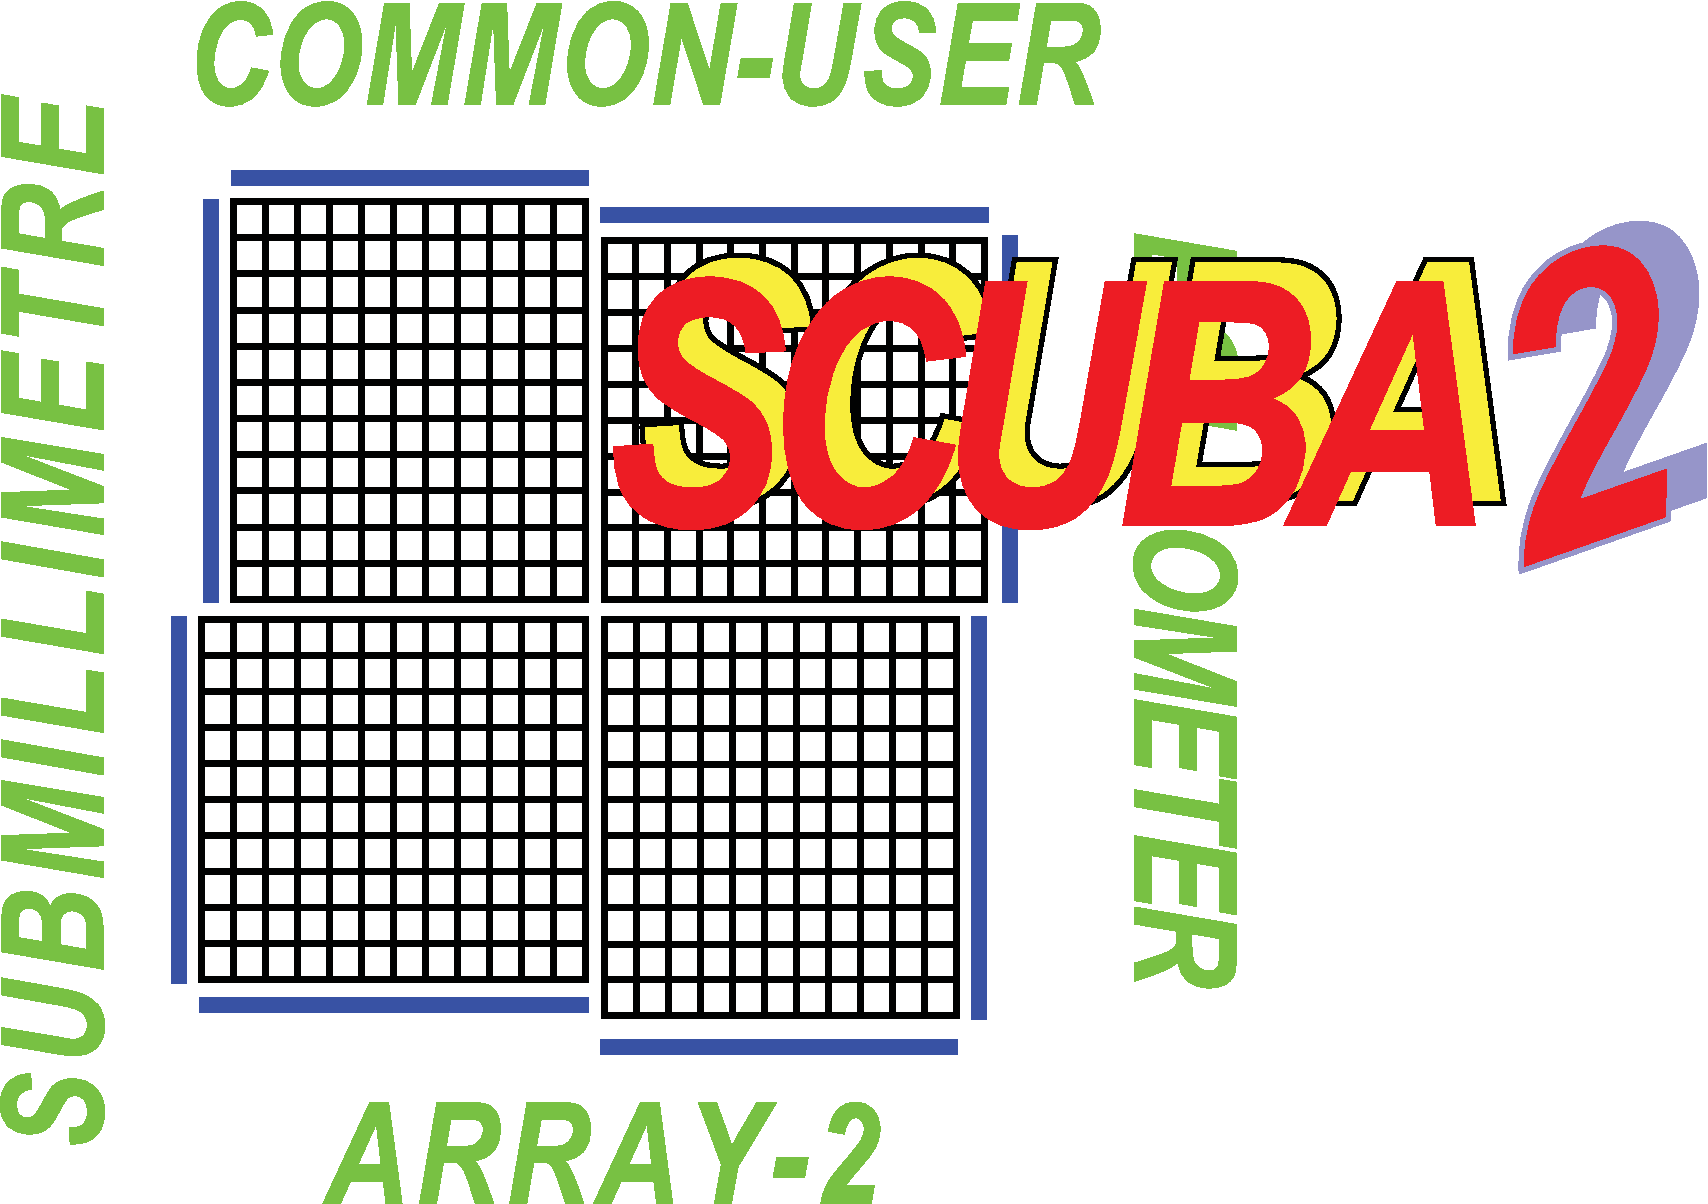
\includegraphics[scale=0.3]{sc19_logo}}
\stardocabstract  {

  This cookbook provides a short introduction to \starlink\ facilities,
  especially \smurf, the Sub-Millimetre User Reduction Facility, for
  reducing and displaying SCUBA-2 SRO data. We describe some of the data
  artefacts present in SCUBA-2 time series and methods we employ to
  mitigate them. In particular, we illustrate the various steps
  required to reduce the data, and the Dynamic Iterative Map-Maker,
  which carries out all of these steps using a single command.

  For information on SCUBA-2 data reduction since SRO, please
  see \xref{SC/21}{sc21}{}.}

% -----------------------------------------------------------------------------
% ? Document specific \providecommand or \newenvironment commands.

%% Upright micron (code stolen from http://www.superstrate.net/useful/useful.html)
\DeclareFontFamily{U}{euc}{}% I chose euc because the chart is called Euler cursive
\DeclareFontShape{U}{euc}{m}{n}{<-6>eurm5<6-8>eurm7<8->eurm10}{}%
\DeclareSymbolFont{AMSc}{U}{euc}{m}{n} % I chose AMSc because AMSa and AMSb are defined in the amsfonts-package
\DeclareMathSymbol{\umu}{\mathord}{AMSc}{"16}

\providecommand{\about}{$\sim$}
\providecommand{\eg}{\textit{e.g.}}
\providecommand{\ie}{\textit{i.e.}}
\providecommand{\micron}{\mbox{\,${\umu}$m}}            % microns
\providecommand{\arcmin}{{$^\prime$}}
\providecommand{\degr}{\mbox{\,$^\circ$}}               % degrees sign

% A new environment for quoting verbatim
% Environment for indenting and using a small font.
\newenvironment{myquote}{\begin{quote}\begin{small}}{\end{small}\end{quote}}

\providecommand{\text}[1]{{\small \texttt{#1}}}

% Typographical shortcuts
\providecommand{\fcfbe}{$\mathrm{FCF_{beamequiv}}$}
\providecommand{\fcfb}{$\mathrm{FCF_{beam}}$}
\providecommand{\fcfa}{$\mathrm{FCF_{arcsec}}$}


% Starlink Package names
\providecommand{\starlink}{\htmladdnormallink{Starlink}{http://starlink.eao.hawaii.edu}}

% set up some common package names
\providecommand{\Kappa}{\xref{\textsc{Kappa}}{sun95}{}}
\providecommand{\cupid}{\xref{\textsc{Cupid}}{sun255}{}}
\providecommand{\Figaro}{\xref{\textsc{Figaro}}{sun86}{}}
\providecommand{\gaia}{\xref{\textsc{Gaia}}{sun214}{}}
\providecommand{\convert}{\xref{\textsc{Convert}}{sun55}{}}
\providecommand{\fluxes}{\xref{\textsc{Fluxes}}{sun213}{}}
\providecommand{\ccdpack}{\xref{\textsc{Ccdpack}}{sun139}{}}
\providecommand{\Iras}{\xref{\textsc{Iras90}}{sun163}{}}
\providecommand{\ndf}{\xref{NDF}{sun33}{}}
\providecommand{\agi}{\xref{AGI}{sun48}{}}
\providecommand{\surf}{\xref{\textsc{Surf}}{sun216}{}}
\providecommand{\Specdre}{\xref{\textsc{Specdre}}{sun140}{}}
\providecommand{\jcmtdr}{\xref{\textsc{JCMTdr}}{sun132}{}}
\providecommand{\nod}{\textsc{nod2}}
\providecommand{\ESP}{\xref{ESP}{sun180}{}}
\providecommand{\GKS}{\xref{GKS}{sun83}{}}
\providecommand{\oracdr}{\xref{\textsc{orac-dr}}{sun231}{}}
\providecommand{\picard}{\xref{\textsc{Picard}}{sun231}{}}
\providecommand{\smurf}{\xref{\textsc{Smurf}}{sun258}{}}
\providecommand{\photom}{\xref{\textsc{Photom}}{sun45}{}}
\providecommand{\topcat}{\htmladdnormallink{\textsc{Topcat}}{http://www.starlink.ac.uk/topcat}}
\providecommand{\ssds}{\xref{\textsc{Starlink Standard Data Structures}}{sgp38}{}}

% DR recipe names
\providecommand{\drrecipe}[1]{\texttt{#1}}

% Application tasks
\providecommand{\task}[1]{\textsf{#1}}

% ADAM parameters
\providecommand{\param}[1]{\texttt{#1}}

% SMURF tasks
\providecommand{\copyflat}{\xref{\task{copyflat}}{sun258}{COPYFLAT}}
\providecommand{\calcflat}{\xref{\task{calcflat}}{sun258}{CALCFLAT}}
\providecommand{\calcnoise}{\xref{\task{calcnoise}}{sun258}{CALCNOISE}}
\providecommand{\concat}{\xref{\task{sc2concat}}{sun258}{SC2CONCAT}}
\providecommand{\fft}{\xref{\task{sc2fft}}{sun258}{SC2FFT}}
\providecommand{\clean}{\xref{\task{sc2clean}}{sun258}{SC2CLEAN}}
\providecommand{\flatfield}{\xref{\task{flatfield}}{sun258}{FLATFIELD}}
\providecommand{\makemap}{\xref{\task{makemap}}{sun258}{MAKEMAP}}
\providecommand{\smurfhelp}{\xref{\task{smurfhelp}}{sun258}{SMURFHELP}}
\providecommand{\jcmtstate}{\xref{\task{jcmtstate2cat}}{sun258}{JCMTSTATE2CAT}}
\providecommand{\smurfsun}{\xref{\textbf{SUN/258}}{sun258}{}}

% Non surf tasks

% KAPPA
\providecommand{\qualtobad}{\xref{\task{qualtobad}}{sun95}{QUALTOBAD}}
\providecommand{\showqual}{\xref{\task{showqual}}{sun95}{SHOWQUAL}}
\providecommand{\display}{\xref{\task{display}}{sun95}{DISPLAY}}
\providecommand{\aperadd}{\xref{\task{aperadd}}{sun95}{APERADD}}
\providecommand{\linplot}{\xref{\task{linplot}}{sun95}{LINPLOT}}
\providecommand{\mlinplot}{\xref{\task{mlinplot}}{sun95}{MLINPLOT}}
\providecommand{\drawsig}{\xref{\task{drawsig}}{sun95}{DRAWSIG}}
\providecommand{\centroid}{\xref{\task{centroid}}{sun95}{CENTROID}}
\providecommand{\hislist}{\xref{\task{hislist}}{sun95}{HISLIST}}
\providecommand{\globals}{\xref{\task{globals}}{sun95}{GLOBALS}}
\providecommand{\setaxis}{\xref{\task{setaxis}}{sun95}{SETAXIS}}
\providecommand{\kstest}{\xref{\task{kstest}}{sun95}{KSTEST}}
\providecommand{\stats}{\xref{\task{stats}}{sun95}{STATS}}
\providecommand{\thresh}{\xref{\task{thresh}}{sun95}{THRESH}}
\providecommand{\setbb}{\xref{\task{setbb}}{sun95}{SETBB}}
\providecommand{\beamfit}{\xref{\task{beamfit}}{sun95}{BEAMFIT}}
\providecommand{\autophotom}{\xref{\task{autophotom}}{sun45}{AUTOPHOTOM}}

\providecommand{\fitslist}{\xref{\task{fitslist}}{sun95}{FITSLIST}}
\providecommand{\fitsedit}{\xref{\task{fitsedit}}{sun95}{FITSEDIT}}

\providecommand{\setvar}{\xref{\task{setvar}}{sun95}{SETVAR}}
\providecommand{\ndfcopy}{\xref{\task{ndfcopy}}{sun95}{NDFCOPY}}
\providecommand{\gdset}{\xref{\task{gdset}}{sun95}{GDSET}}
\providecommand{\idset}{\xref{\task{idset}}{sun95}{IDSET}}
\providecommand{\ovset}{\xref{\task{ovset}}{sun95}{OVSET}}
\providecommand{\gdnames}{\xref{\task{gdnames}}{sun95}{GDNAMES}}
\providecommand{\gdclear}{\xref{\task{gdclear}}{sun95}{GDCLEAR}}
\providecommand{\cursor}{\xref{\task{cursor}}{sun95}{CURSOR}}
\providecommand{\flip}{\xref{\task{flip}}{sun95}{FLIP}}
\providecommand{\cadd}{\xref{\task{cadd}}{sun95}{CADD}}

\providecommand{\cdiv}{\xref{\task{cdiv}}{sun95}{CDIV}}
\providecommand{\Div}{\xref{\task{div}}{sun95}{DIV}}
\providecommand{\cmult}{\xref{\task{cmult}}{sun95}{CMULT}}
\providecommand{\mult}{\xref{\task{mult}}{sun95}{MULT}}
\providecommand{\add}{\xref{\task{add}}{sun95}{ADD}}
\providecommand{\sub}{\xref{\task{sub}}{sun95}{SUB}}
\providecommand{\csub}{\xref{\task{csub}}{sun95}{CSUB}}
\providecommand{\psf}{\xref{\task{psf}}{sun95}{PSF}}

\providecommand{\glitch}{\xref{\task{glitch}}{sun95}{GLITCH}}
\providecommand{\setunits}{\xref{\task{setunits}}{sun95}{SETUNITS}}
\providecommand{\fitstext}{\xref{\task{fitstext}}{sun95}{FITSTEXT}}
\providecommand{\fitsmod}{\xref{\task{fitsmod}}{sun95}{FITSMOD}}
\providecommand{\fitshead}{\xref{\task{fitshead}}{sun95}{FITSHEAD}}
\providecommand{\lutbgyrw}{\xref{\task{lutbgyrw}}{sun95}{LUTBGYRW}}
\providecommand{\contour}{\xref{\task{contour}}{sun95}{CONTOUR}}
\providecommand{\contover}{\xref{\task{contover}}{sun95}{CONTOVER}}

\providecommand{\turbocont}{\xref{\task{turbocont}}{sun95}{TURBOCONT}}
\providecommand{\mosaic}{\xref{\task{mosaic}}{sun95}{MOSAIC}}
\providecommand{\pixdupe}{\xref{\task{pixdupe}}{sun95}{PIXDUPE}}
\providecommand{\rotate}{\xref{\task{rotate}}{sun95}{ROTATE}}
\providecommand{\setbound}{\xref{\task{setbound}}{sun95}{SETBOUND}}
\providecommand{\slide}{\xref{\task{slide}}{sun95}{SLIDE}}
\providecommand{\gausmooth}{\xref{\task{gausmooth}}{sun95}{GAUSMOOTH}}
\providecommand{\median}{\xref{\task{median}}{sun95}{MEDIAN}}

\providecommand{\memd}{\xref{\task{mem2d}}{sun95}{MEM2D}}
\providecommand{\axlabel}{\xref{\task{axlabel}}{sun95}{AXLABEL}}
\providecommand{\axunits}{\xref{\task{axunits}}{sun95}{AXUNITS}}
\providecommand{\setlabel}{\xref{\task{setlabel}}{sun95}{SETLABEL}}
\providecommand{\settitle}{\xref{\task{settitle}}{sun95}{SETTITLE}}
\providecommand{\histogram}{\xref{\task{histogram}}{sun95}{HISTOGRAM}}
\providecommand{\normalize}{\xref{\task{normalize}}{sun95}{NORMALIZE}}

\providecommand{\ndftrace}{\xref{\task{ndftrace}}{sun95}{NDFTRACE}}
\providecommand{\fitsval}{\xref{\task{fitsval}}{sun95}{NDFTRACE}}

\providecommand{\makesnr}{\xref{\task{makesnr}}{sun95}{MAKESNR}}
\providecommand{\wcsmosaic}{\xref{\task{wcsmosaic}}{sun95}{WCSMOSAIC}}
\providecommand{\mfittrend}{\xref{\task{mfittrend}}{sun95}{MFITTREND}}

% Convert
\providecommand{\ndffits}{\xref{\task{ndf2fits}}{sun55}{NDF2FITS}}
\providecommand{\ndfascii}{\xref{\task{ndf2ascii}}{sun55}{NDF2ASCII}}

% FIGARO
\providecommand{\wdfits}{\xref{\task{wdfits}}{sun86}{WDFITS}}
\providecommand{\istat}{\xref{\task{istat}}{sun86}{ISTAT}}
\providecommand{\delobj}{\xref{\task{delobj}}{sun86}{DELOBJ}}
\providecommand{\copobj}{\xref{\task{copobj}}{sun86}{COPOBJ}}
\providecommand{\image}{\xref{\task{image}}{sun86}{IMAGE}}
\providecommand{\bclean}{\xref{\task{bclean}}{sun86}{BCLEAN}}
\providecommand{\ystract}{\xref{\task{ystract}}{sun86}{YSTRACT}}
\providecommand{\sclean}{\xref{\task{sclean}}{sun86}{SCLEAN}}

% CCDPACK
\providecommand{\makemos}{\xref{\task{makemos}}{sun139}{MAKEMOS}}

% IRAS90
\providecommand{\skypos}{\xref{\task{skypos}}{sun163}{SKYPOS}}
\providecommand{\skygrid}{\xref{\task{skygrid}}{sun163}{SKYGRID}}
\providecommand{\skyphot}{\xref{\task{skyphot}}{sun163}{SKYPHOT}}

% CUPID
\providecommand{\findback}{\xref{\task{findback}}{sun255}{FINDBACK}}

% Misc
\providecommand{\hdstrace}{\xref{\task{hdstrace}}{sun102}{}}
\providecommand{\psmerge}{\xref{\task{psmerge}}{sun164}{}}
\providecommand{\fitgauss}{\xref{\task{fitgauss}}{sun140}{FITGAUSS}}
\providecommand{\gaufit}{\xref{\task{gaufit}}{sun180}{GAUFIT}}

% ? End of document specific commands
% -----------------------------------------------------------------------------
%  Title Page.
%  ===========
\begin{document}
\scfrontmatter


\section{\xlabel{introduction}Introduction}
\label{sec:intro}

The Submillimetre Common User Bolometer Array-2 (SCUBA-2) is a
large-format bolometer camera for the 15-m James Clerk Maxwell
Telescope, designed to produce simultaneous continuum images with
central wavelengths at 450 and 850\micron.

The purpose of this guide is to help SCUBA-2 users become familiar
with the basic facilities for analysing and visualising data using
\smurf \cite{smurf}, and the \starlink\ packages \Kappa \cite{kappa},
and \gaia \cite{gaia}. Obviously, \starlink\ must be installed on your
system, and \starlink\ aliases and environment variables must be
defined before attempting any of the examples in this document.  This
guide is \emph{not} aimed at users of the polarimeter (POL-2) or
Fourier transform spectrometer (FTS-2).

A brief description of raw SCUBA-2 data is given in
Section~\ref{sec:data}. Section~\ref{sec:visual} demonstrates how to
visualise SCUBA-2 data, interspersed with some simple worked examples
of interactive data-reduction techniques. The end goal of this section
is \emph{not} to produce a final science-grade map, rather to give the
user a feel for the types of artefacts and data reduction steps
required to make a useful image. The best way to make an image from
SCUBA-2 data is to use the Dynamic Iterative Map-Maker (DIMM). This
one-line command and a subset of its control parameters are described
in Section~\ref{sec:maps}. We then discuss data calibration
(\S\ref{sec:calib}) and provide worked examples of cosmology
(\S\ref{sec:cosmology}) and Galactic (\S\ref{sec:galactic}) data
reduction. For the user who wishes only to produce maps in as little
time as possible, jump straight to these later sections.

Note that a number of the examples in this document use real data that
are distributed with this \starlink\ release. The small Uranus example
is distributed as part of SMURF and can be found in:

\begin{terminalv}
$STARLINK_DIR/share/smurf/s4a20091214_00015_000*.sdf
\end{terminalv}

The more detailed examples use larger data sets which, because of
their size, can be downloaded separately via the URL
\htmladdnormallink{http://www.starlink.ac.uk/extras/sc19/}{http://www.starlink.ac.uk/extras/sc19/}.
If you wish to use these data for scientific purposes (i.e. leading to
a publication), explicit permission must be obtained from the Director
of the James Clerk Maxwell Telescope.

To gain access to \smurf\ tasks (the data reduction package for
SCUBA-2) before proceeding with the examples in this document first
type:

\begin{terminalv}
% smurf


        SMURF commands are now available -- (Version 1.3.1)

        Type smurfhelp for help on SMURF commands.
        Type 'showme sun258' to browse the hypertext documentation.
        Type 'showme sc19' to view the SCUBA-2 map-making cookbook.


\end{terminalv}
%

For a more detailed description refer to the comprehensive Starlink
User Note (\smurfsun)\footnote{currently SUN/258 is not completely up
  to date}.


\section{\xlabel{data_files}SCUBA-2 Data Files}
\label{sec:data}

The SCUBA-2 data acquisition (DA) system writes data files every
30\,s, one file for each of the $40\times32$ pixel subarrays. In
addition, each observation can be preceded or followed by calibration
frames such as darks or flatfield ramps. For example, observation 15
on 2009-12-14 of Uranus produced the following 16 files with the
450\micron\ array that was operational at the time (s4a):

\begin{small}
\begin{terminalv}
-rw-r--r-- 1 echapin software  5976576 Jan 17 08:01 s4a20091214_00015_0001.sdf
-rw-r--r-- 1 echapin software 34945536 Jan 17 08:01 s4a20091214_00015_0002.sdf
-rw-r--r-- 1 echapin software 34945536 Jan 17 08:01 s4a20091214_00015_0003.sdf
-rw-r--r-- 1 echapin software 34945536 Jan 17 08:01 s4a20091214_00015_0004.sdf
-rw-r--r-- 1 echapin software 34945536 Jan 17 08:02 s4a20091214_00015_0005.sdf
-rw-r--r-- 1 echapin software 34945536 Jan 17 08:02 s4a20091214_00015_0006.sdf
-rw-r--r-- 1 echapin software 34945536 Jan 17 08:02 s4a20091214_00015_0007.sdf
-rw-r--r-- 1 echapin software 34945536 Jan 17 08:02 s4a20091214_00015_0008.sdf
-rw-r--r-- 1 echapin software 34945536 Jan 17 08:02 s4a20091214_00015_0009.sdf
-rw-r--r-- 1 echapin software 34945536 Jan 17 08:02 s4a20091214_00015_0010.sdf
-rw-r--r-- 1 echapin software 34945536 Jan 17 08:02 s4a20091214_00015_0011.sdf
-rw-r--r-- 1 echapin software 34945536 Jan 17 08:02 s4a20091214_00015_0012.sdf
-rw-r--r-- 1 echapin software 34945536 Jan 17 08:02 s4a20091214_00015_0013.sdf
-rw-r--r-- 1 echapin software 34945536 Jan 17 08:02 s4a20091214_00015_0014.sdf
-rw-r--r-- 1 echapin software 11778560 Jan 17 08:02 s4a20091214_00015_0015.sdf
-rw-r--r-- 1 echapin software  5977600 Jan 17 08:02 s4a20091214_00015_0016.sdf
\end{terminalv}
\end{small}

The fifth column gives the file sizes in bytes, and shows that the
first and last files, which were dark observations, have nearly
identical lengths. Similarly files 2 to 14 also have identical sizes
as they each contain precisely 30\,s worth of the on-source
integration. File 15 is shorter, as the end of the integration lasted
less than 30\,s.  As noted in the introduction, the first two files
containing data from the actual scan of Uranus (numbers 2 and 3) are
included with this \starlink\ release.

\Kappa\ tasks such as \fitslist\ and \ndftrace\ can be used to see the
FITS headers and dimensions of the data. In this example, the first
and last files are dark observations, and all the other files are
produced by a single continuous scan of Uranus. The main data arrays
of each file are cubes, with the first two dimensions enumerating
columns and rows, and the third time slices (sampled at 200\,Hz).

Raw SCUBA-2 data are stored as integers (uncalibrated digitized
units). The \smurf\ task \flatfield\ can be used to scale raw data to
units proportional to picowatts (pW, as double precision floating
points) using the results of measurements of a flatfield
calibration. The calibration can be stored internally in the data file
(see the HDS extension \texttt{MORE.SCUBA2.FLATCAL}) or can be
calculated dynamically from the flatfield ramps bracketing each
science observation. The DIMM will always use a flatfield ramp if
available. For example, use the command

\begin{terminalv}
% flatfield 's4a20091214_00015_*.sdf' '*_flat'
\end{terminalv}
%
to produce flat-fielded versions of the files that contain bolometer
data taken during the scan across Uranus, with the dark observations
(1 and 16 in this example) automatically filtered out. Other
non-science files will also be ignored\footnote{Use the SEQ\_TYPE FITS
  header to determine whether a file is part of the main data
  acquisition sequence or a support file}. Note that the single quotes
around the wildcards for the input and output files are necessary
since \starlink\ routines expand them internally, rather than using
the shell. However, it is not generally necessary to use \flatfield\
before proceeding with map-making. \smurf\ will flatfield the data
internally by default.

\section{\xlabel{time_series}Visualising data}
\label{sec:visual}

In this section several procedures are described for looking at
SCUBA-2 data, as well as basic data reduction steps that can be run
separately. Working through these examples will illustrate some of the
features of SCUBA-2 data, but will \emph{not} result in a science-grade
image at the end. If you are interested only in making the best
possible map with minimal effort proceed to Section~\ref{sec:maps}.

\subsection{\xlabel{concat}Concatenating data}

Since SCUBA-2 data for a given subarray are broken into many pieces by
the DA system, it is useful for visualisation to first concatenate the
data into single files. The \smurf\ task \concat\ can be used for this
operation. For example, assuming the following files are in the
current working directory,

\begin{terminalv}
% sc2concat 's4a20091214_00015_00??.sdf' './*_con'
\end{terminalv}

combines all of the files associated with observation 15 for the s4a
array into a single file called
s4a20091214\_00015\_0002\_con.sdf. \concat\ will automatically filter
out any dark observations, so that the concatenated file contains only
the data taken during the scan across Uranus with the shutter open. It
also applies the flatfield by default, although it can be disabled using
the `noflat' option on the command-line. Be careful when concatenating
a very long observation since the output file may be too large to
handle sanely. Fifteen minute chunks (30 files) should be more than
big enough.

\subsection{\xlabel{display_scan}Displaying scan patterns}
\label{sec:state}

The pointing of the telescope throughout a scan (as well as other
state information) is stored in the \texttt{MORE.SMURF.JCMTSTATE}
extension of a data file. The \smurf\ task \jcmtstate\ will convert
this information into a simple ASCII tab separated table:

\begin{terminalv}
% jcmtstate2cat s4a20091214_00015_0002_con.sdf > state.tst
\end{terminalv}

\begin{figure}
\begin{center}
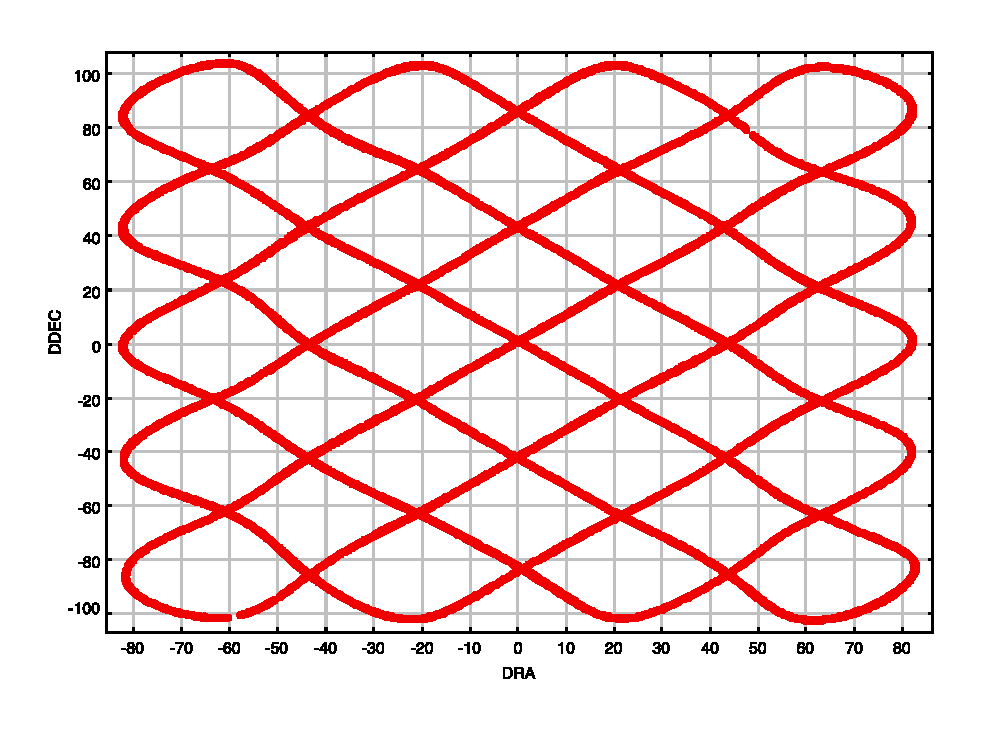
\includegraphics{sc19_scan_pattern}
\caption{The telescope positions during observation number 7 on
  20090107. The plot is created by \topcat\ from the output from
  \jcmtstate\ plotting the DRA column (right ascension offset from the
  map centre in arcsec) against the DDEC column (declination offset
  from the map centre in arcsec). The PONG scan pattern is clearly
  visible (see Scott \& Engelen 2008\cite{sc2ana005}).}
\label{fig:topcat}
\end{center}
\end{figure}

The `-h' option to \jcmtstate\ can be used to find more information on
the command. In particular, multiple files can be supplied to the
command using standard shell wild cards (not escaped) and for SCUBA-2
data the `--with-mce' option can be used to dump the low-level MCE
header information.

This catalogue can be loaded into \topcat\ for plotting, making sure
that \topcat\ is told that the TST format is to be used for reading.

\begin{terminalv}
% topcat -f tst state.tst
\end{terminalv}

An example plot of the scan pattern for this observation generated by
\topcat\ can be seen in Fig.~\ref{fig:topcat}. All the time varying
header values are available for plotting. In particular DRA and DDEC
will show the RA/Dec offset of the telescope, DAZ and DEL will show
the Az/El offset and the 225\,GHz opacity values are also calculated
from the raw WVM measurements.

\subsection{\xlabel{display_cube}Displaying data cubes}
\label{sec:gaiacube}

\begin{figure}
\begin{center}
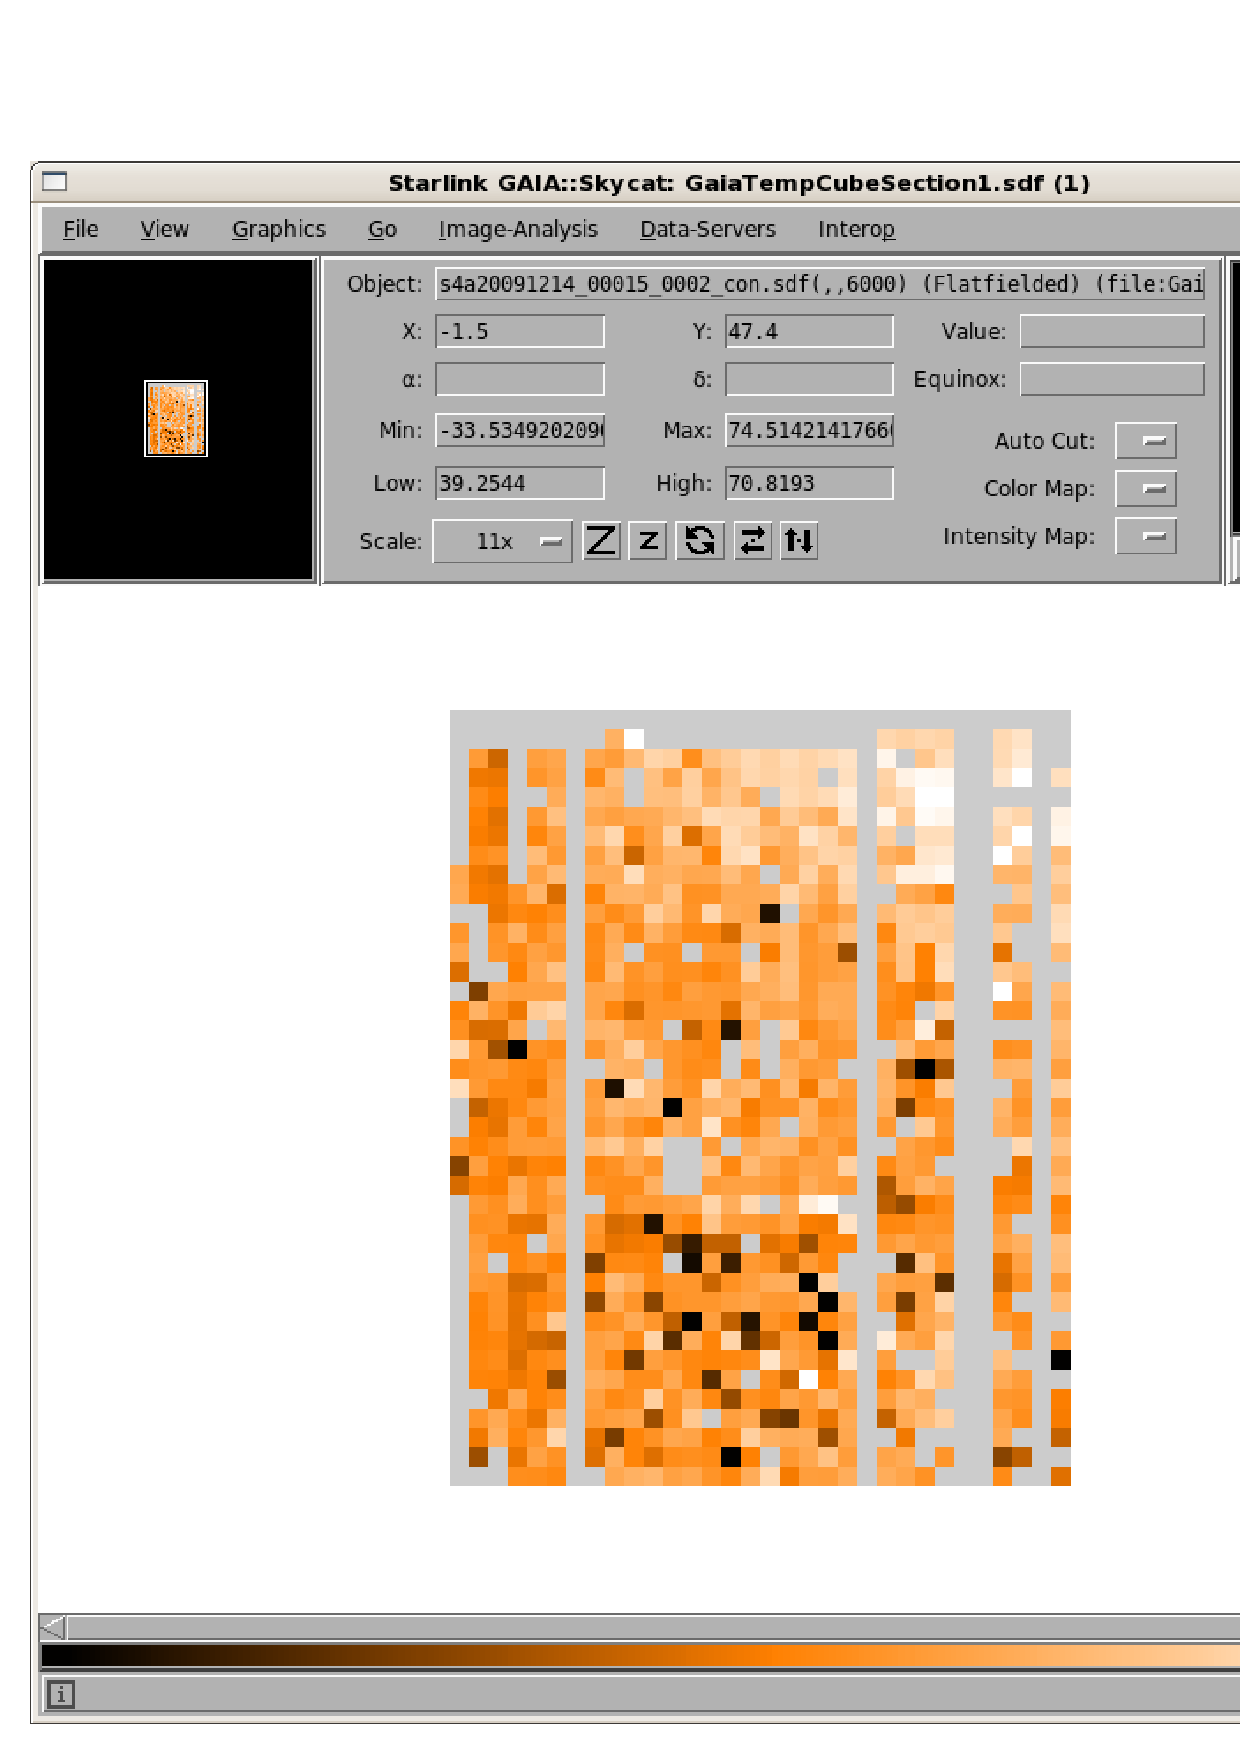
\includegraphics[width=0.61\linewidth]{sc19_gaia_main}\hspace{0.03\linewidth}
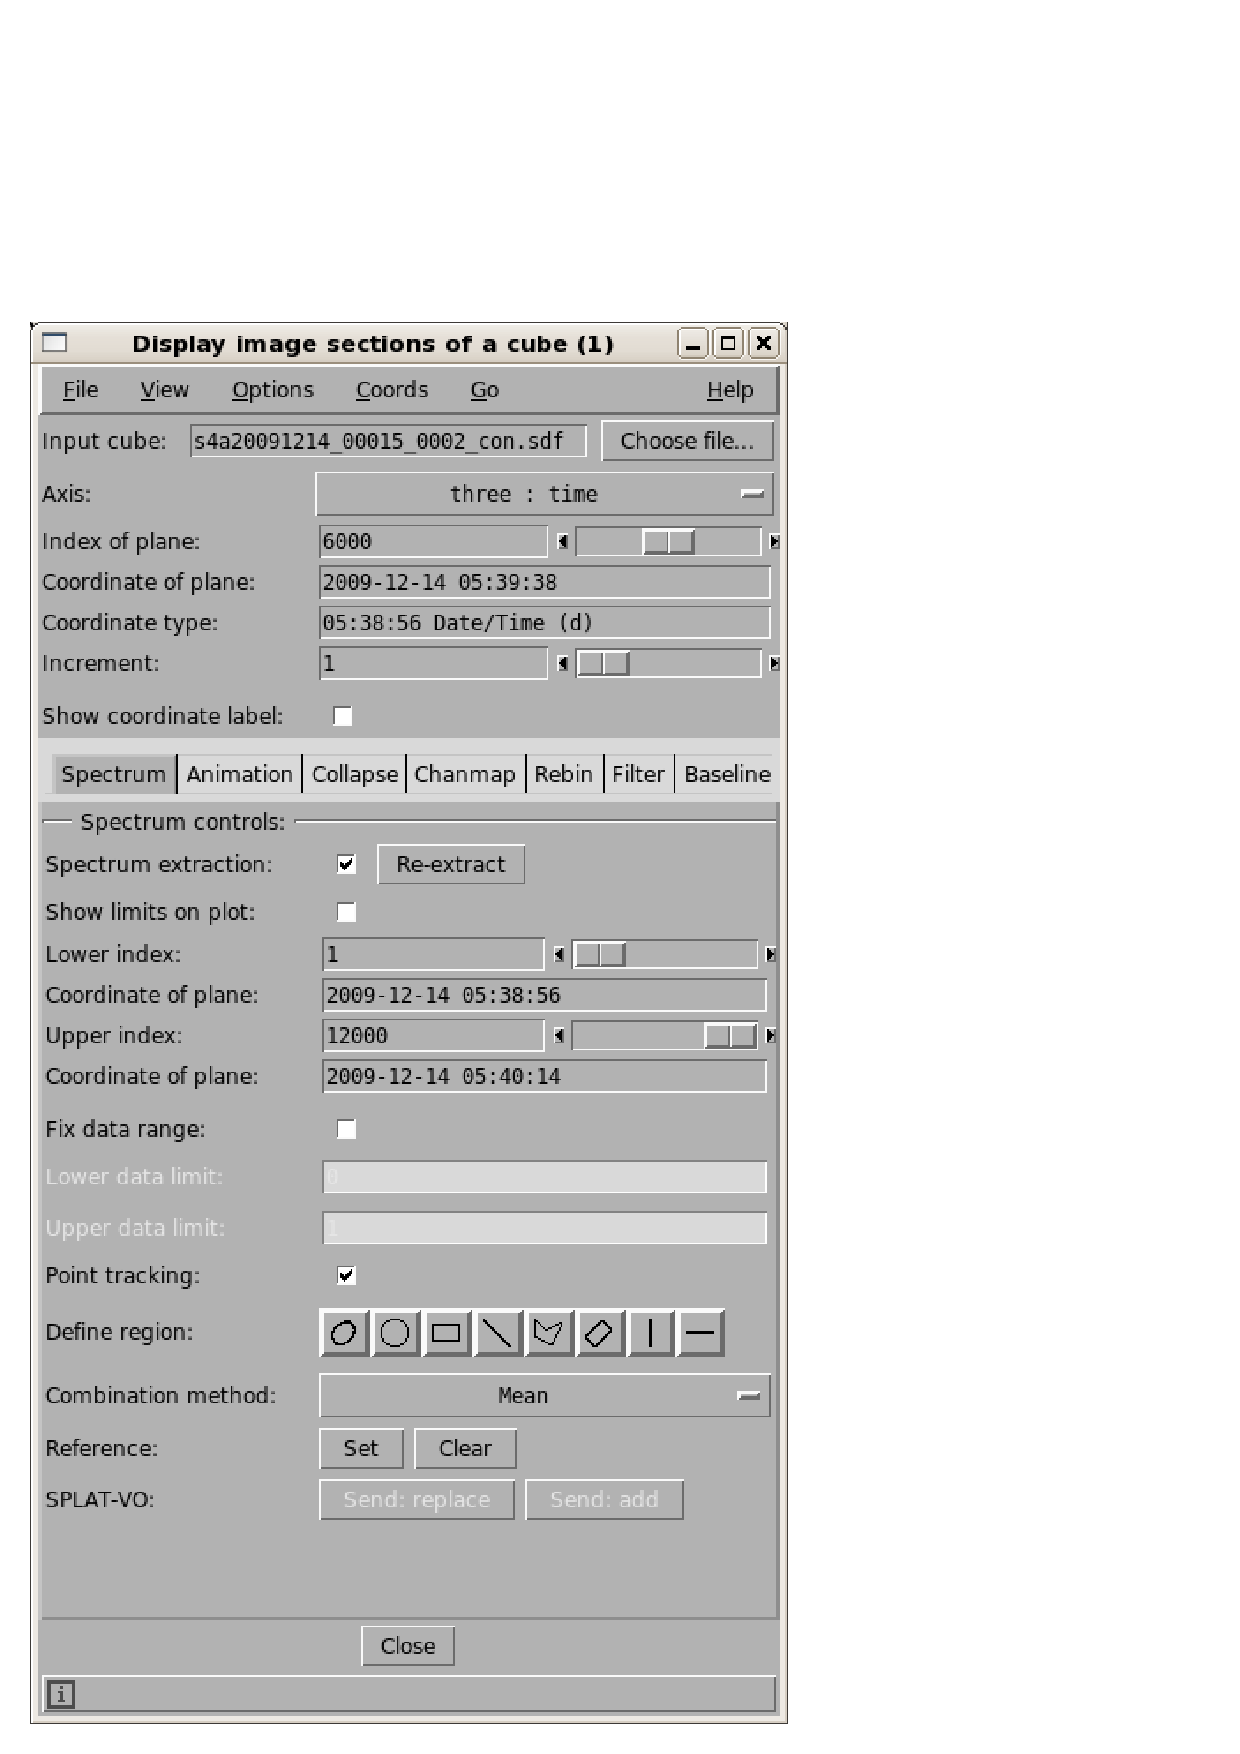
\includegraphics[width=0.33\linewidth]{sc19_gaia_sections}
\caption{Initial \gaia\ windows displayed upon loading a data cube
  (with slight modifications to the colour table using options under
  the `File' and then `Startup options'). \textbf{Left:} The main
  window, after clicking the `Z' button a number of times to zoom-in,
  shows a map of bolometer values at a fixed sample in time. Note that
  these data came from an array with a number of broken columns and
  broken isolated bolometers, all indicated in grey. \textbf{Right:} The
  `Display image sections of a cube' dialogue enables the user to
  navigate the time dimension. The `Index of plane' slider near the
  top can be used to select different time slices, and the main window
  will automatically update.}
\label{fig:gaia_main}
\end{center}
\end{figure}

The easiest way to visualise the bolometer time series data is to use
\gaia. Loading in the concatenated file above (combining the two
example files included with this \starlink\ release) produces two
windows (Fig.~\ref{fig:gaia_main}). The main window shows a map of
bolometer values at a given instant in time. The second window can be
used to navigate the time axis; by moving the `Index of plane' slider
in the `Display image sections of a cube' dialogue, different time
slices may be selected, with the main \gaia\ window updating
automatically.

For this concatenated data file (1\,minute in total, as it is the
combination of two 30\,s files), each bolometer has a large offset
relative to its neighbours as well as relative to any smaller
time-varying signals, which means that little difference can be seen
by moving the slider. However, \gaia\ can produce an automatically
scaled plot of the time series for an individual bolometer by simply
clicking on it in the main window. For example, clicking on the
bolometer at (13,23) spawns the `Spectral plot'\footnote{This feature
  of \gaia\ was originally developed to display spatially-resolved
  spectra stored in data cubes, hence the name, `Spectral plot'.}
window shown in Fig.~\ref{fig:gaia_spec} for a single
bolometer. Clicking on other bolometers over-writes the plot of the
original bolometer in the same window. Looking at the vertical axis
range on the left, the mean levels clearly vary significantly from
bolometer to bolometer, although the time-varying component of the
signals are quite similar.

\begin{figure}
\begin{center}
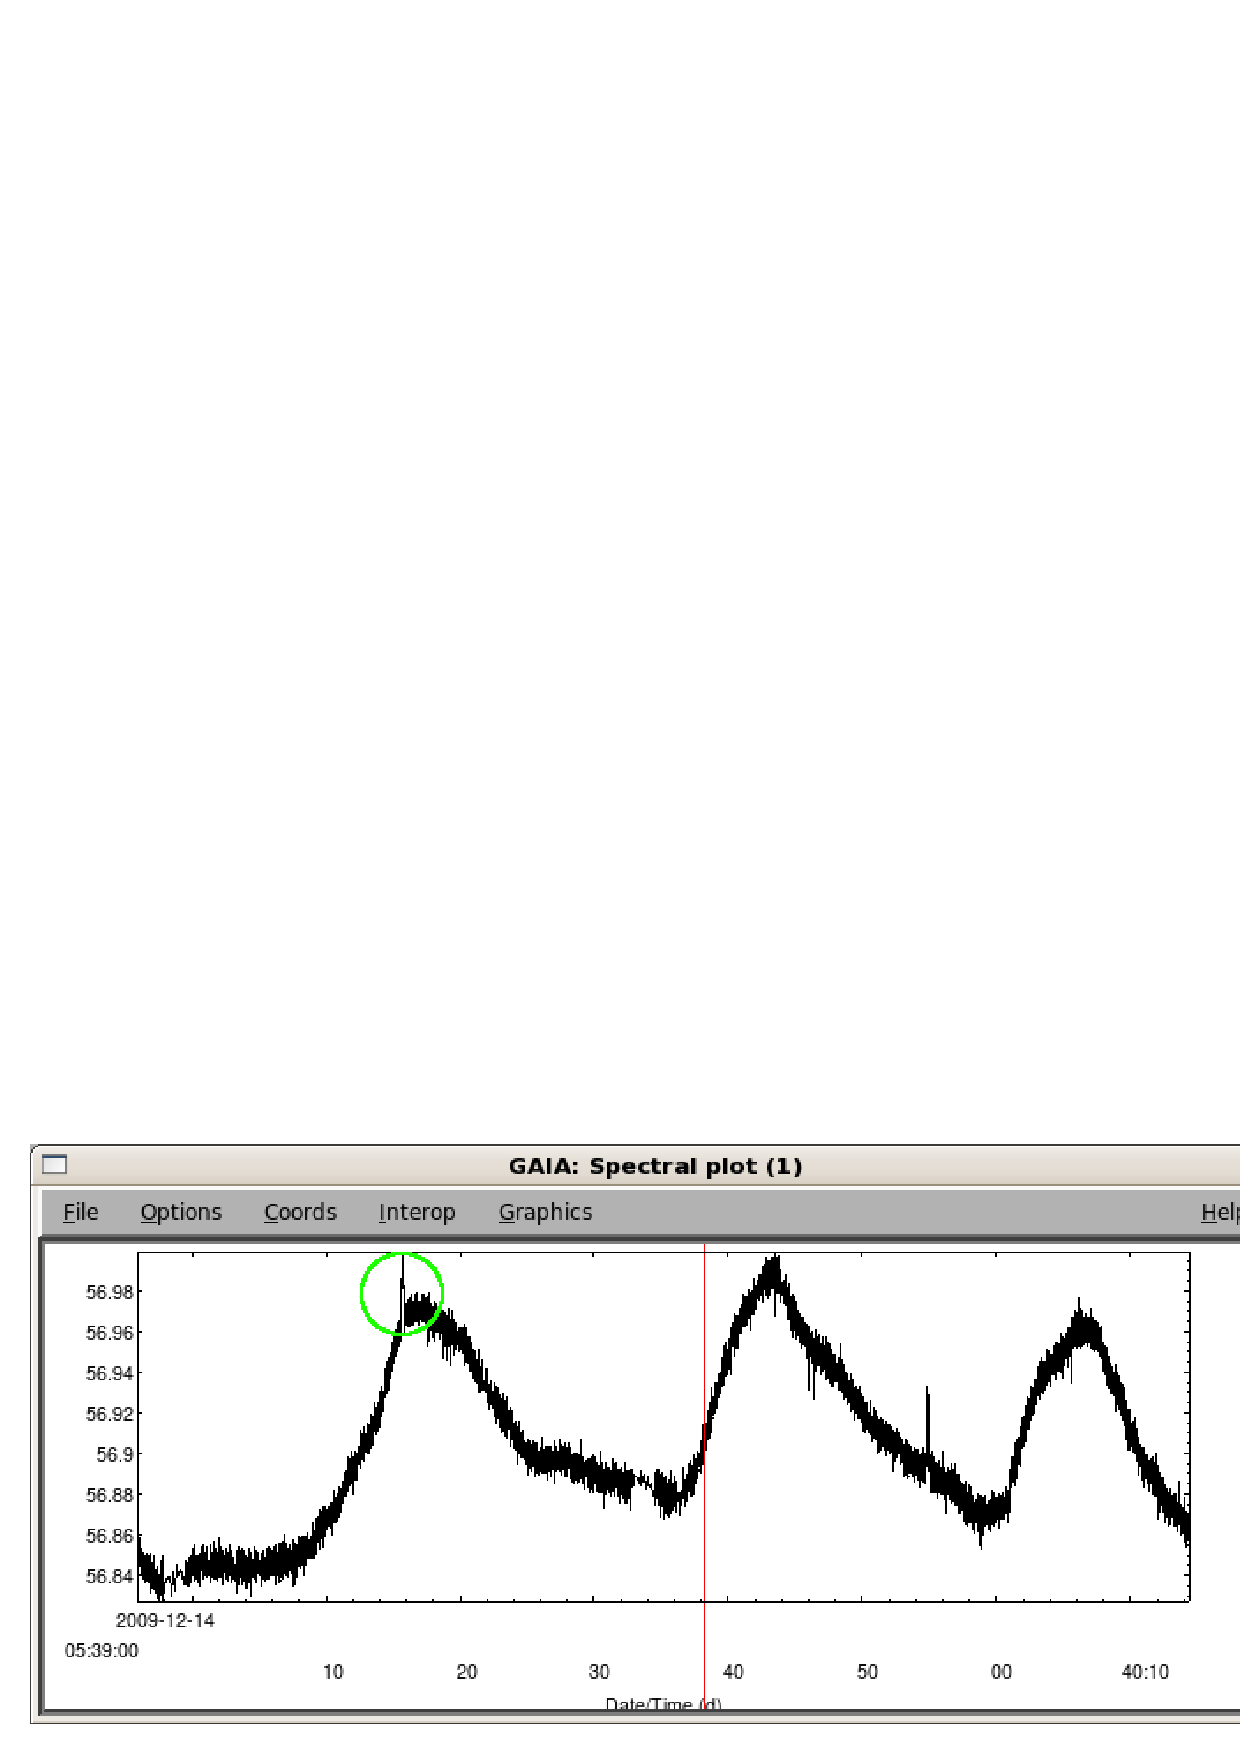
\includegraphics[width=0.7\linewidth]{sc19_gaia_spec}
\caption{The `Spectral Plot' window is spawned automatically once a
  bolometer is clicked in the main window, such as (13,23) in this
  example, displaying its time-varying signal. The vertical red line
  indicates the time slice that is currently selected in the `Display
  image sections of a cube' dialogue. The regular pattern, with a
  period of about 30 seconds in this particular case, is slow baseline
  drift correlated with variations in the SCUBA-2 fridge
  temperature. The green-circled narrow spike is produced by the
  bolometer crossing Uranus. Usually astronomical signals are not
  readily visible in raw time series plots such as these, since they
  are relatively much fainter. Note that on some systems `gaps' may
  appear, such as those at the start of the time series, and at
  $\sim34$\,s in this example. These are simply rendering artefacts
  due to re-sampling the data to the resolution of the display
  (zooming-in to these regions using the `Lower index' and `Upper
  index' sliders in the `Display image sections of a cube' dialogue
  followed by a click on `Re-extract' to update the plot demonstrates
  this).}
\label{fig:gaia_spec}
\end{center}
\end{figure}

\subsection{\xlabel{regrid_map}Regridding data into a map}

A simple and quick map can be made from a data cube using the \smurf\
\makemap\ task. The following will produce a map directly from the raw
concatenated data by re-gridding it into a pixelated map:

\begin{terminalv}
% makemap s4a20091214_00015_0002_con.sdf uranus method=rebin
\end{terminalv}

The \makemap\ task automatically scales the bounds of the image to
encompass all of the data. The output map here is called
`\texttt{uranus.sdf}', and the pixel scale is 2~arcsec on a side by
default at 450\micron\ and 4~arcsec at 850\micron\ (although this can
be changed using the `pixsize=$x$' option on the command-line, where
$x$ is in arcsec)\footnote{The default sizes are defined as one
  quarter of the Airy disk rounded up to the nearest half
  arcsecond.}. Since we already know that relative bolometer offsets
are large in these data, it is unsurprising that no astronomical
source can be seen with \gaia\ in the resulting image.

\begin{figure}
\begin{center}
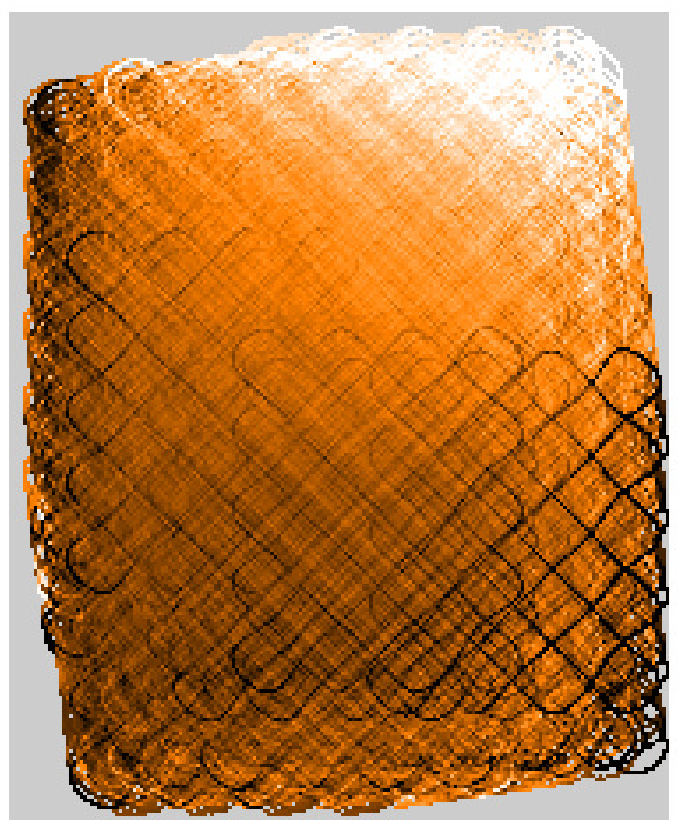
\includegraphics[width=0.5\linewidth]{sc19_rawmap}
\caption{Map produced from raw data of a scan across Uranus. The
  image is completely dominated by noise in the relative signal
  offsets of each bolometer, and no astronomical signal can be
  seen. The scan (a Curvy PONG) can clearly be seen as a repetitive
  `waffle' pattern in the image.}
\label{fig:rawmap}
\end{center}
\end{figure}

\subsection{\xlabel{clean}Cleaning data}

The previous examples illustrate the need for some kind of data
cleaning before there is any hope of seeing astronomical sources. A
useful \smurf\ task for time-domain data processing is \clean, which
can perform several different steps controlled by a range of
parameters. Note that all of the algorithms available to \clean\ are
also accessible within the DIMM (Section~\ref{sec:maps}), so in
practice the user does not issue this command directly before making
the final map.

\subsubsection{\xlabel{clean_average}Removing bolometer averages and DC Steps}

The following will remove a 0th-order polynomial (the mean) from each
bolometer time stream, storing the cleaned data in a file called
`clean.sdf':

\begin{terminalv}
% sc2clean s4a20091214_00015_0002_con.sdf clean \
     config="order=0"
\end{terminalv}

\begin{figure}
\begin{center}
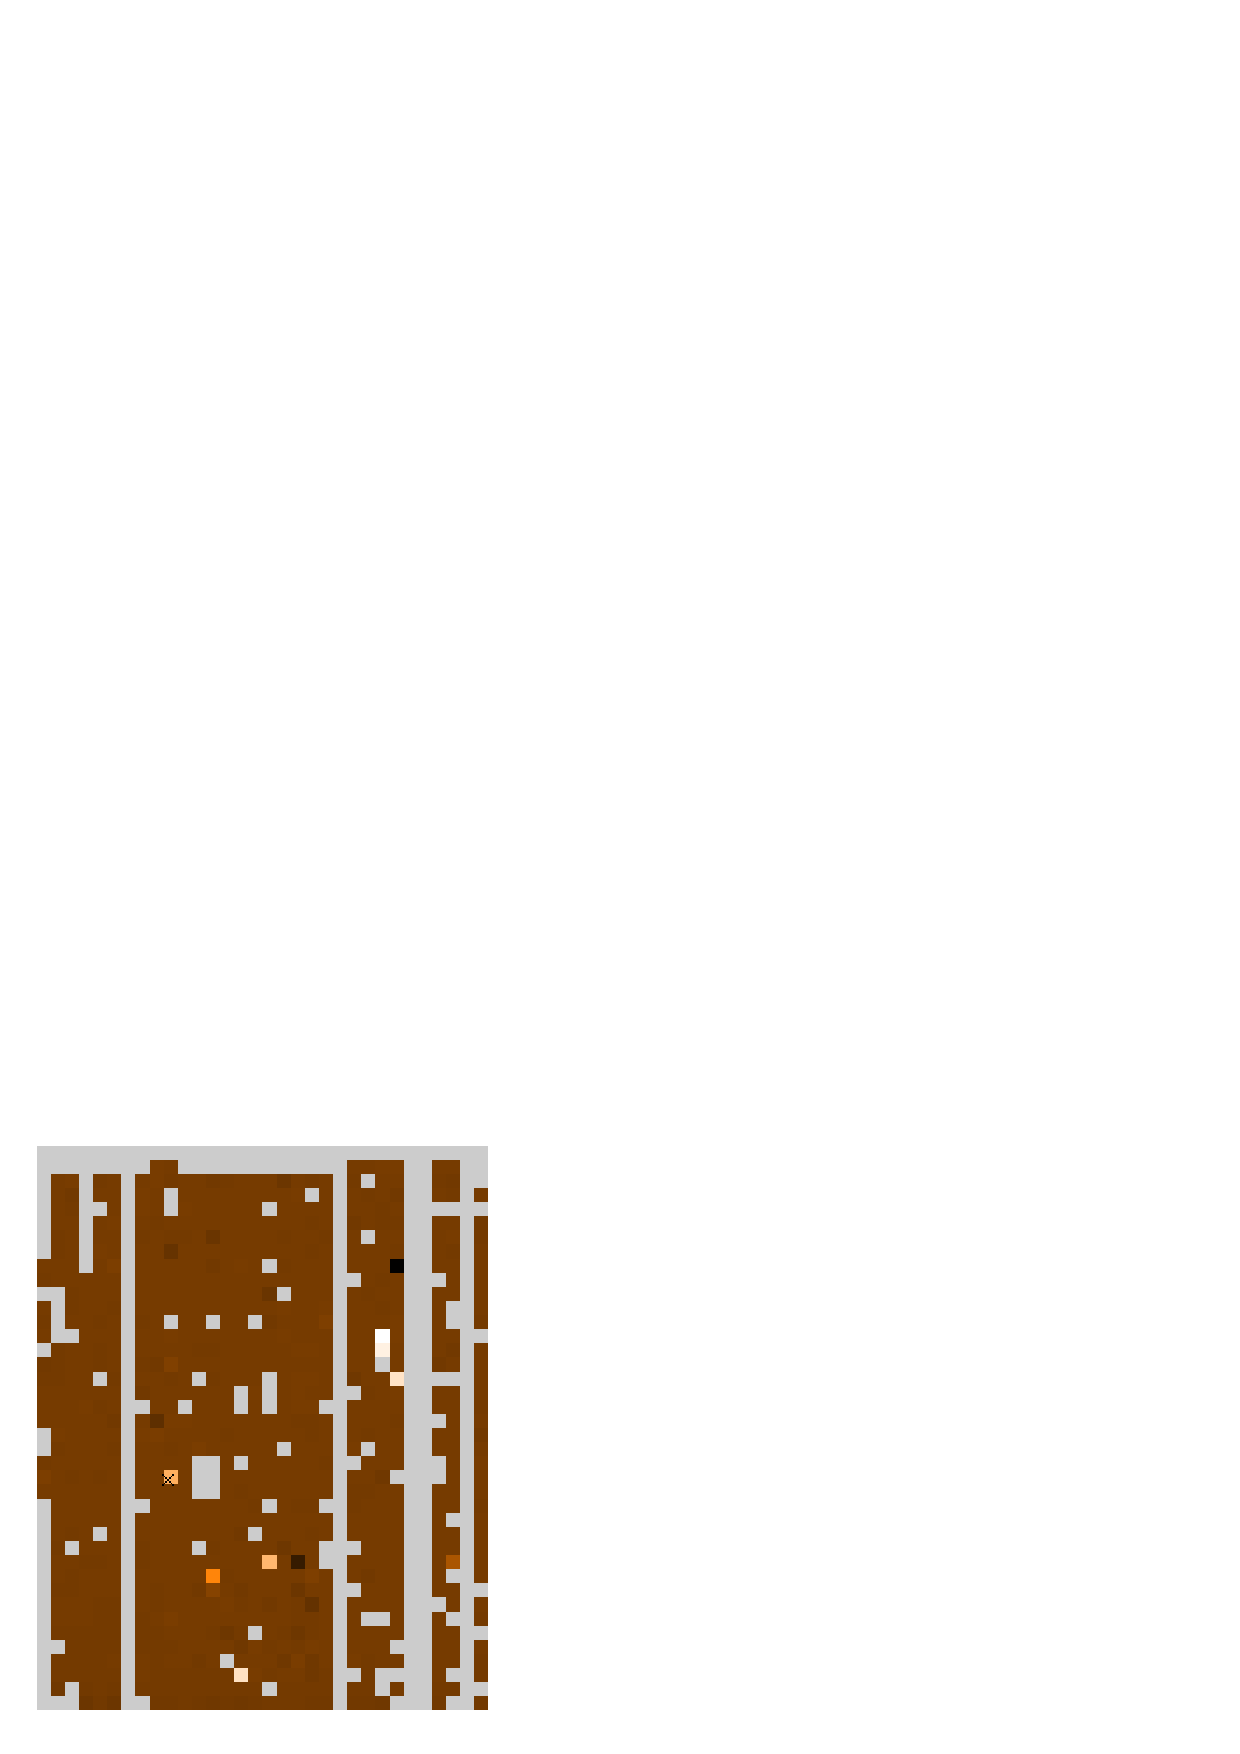
\includegraphics[width=0.5\linewidth]{sc19_array_mean}
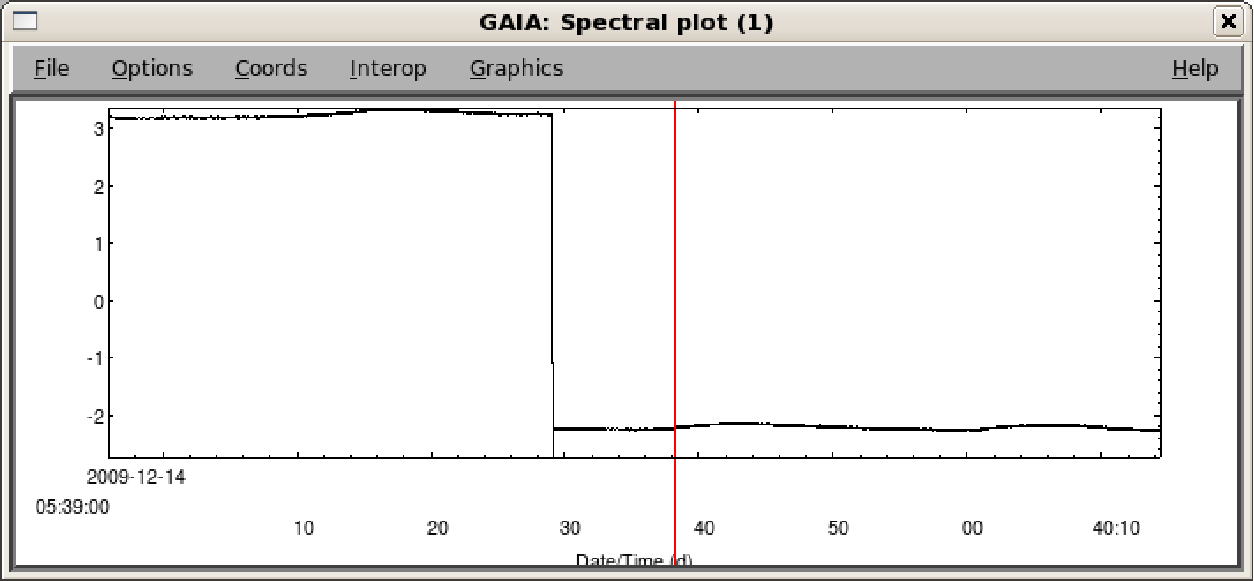
\includegraphics[width=0.9\linewidth]{sc19_dcstep}
\caption{\textbf{Top:} \gaia\ plot of the array signal at time slice 1
  after using \clean\ to remove the mean of each bolometer signal
  (clean.sdf). The LOW and HIGH data values for this intensity plot
  are $-1.7171$\,pW and $+5.50352$\,pW, respectively. Most of the
  working bolometers (not grey) now have approximately the same signal
  range (approximately $\pm 0.1$\,pW), and therefore have nearly the
  same colour (brown). However, there are several outliers, for
  example, the orange pixel with an `x' at (10,17). \textbf{Bottom:} The
  time series for bolometer (10,17) showing the presence of a large
  level change, or `DC Step' near 30\,s.}
\label{fig:array_mean}
\end{center}
\end{figure}

This operation results in bolometer data that lie primarily in the
range $\pm 0.1$\,pW, except for a handful of outliers as shown in
Fig.~\ref{fig:array_mean}. In these cases there have been large level
changes, or `DC Steps', during data acquisition. These can
be identified and repaired using some extra parameters to \clean:

\begin{terminalv}
% sc2clean s4a20091214_00015_0002_con.sdf clean2 \
   config='"order=0,dcfitbox=30,dcthresh=25,dcsmooth=50"'
\end{terminalv}

In addition to removing the mean as in the previous example, the extra
parameters starting with `dc' instruct \clean\ to smooth the data with
a median filter of width 50 samples, and then look for steps in the
smoothed data in excess of 25-$\sigma$. The heights of steps found in
this way are measured by fitting straight lines to the smoothed data
on either side of the jump using 30 samples in each fit. The
corrections thus determined are applied to the original bolometer
data.  Note that an additional flag has been set by default,
\texttt{fillgaps=1}, indicating that the data range around the
identified steps ($\pm 400$ samples in this case) should be replaced
with a constrained (smooth) realisation of noise to avoid introducing
spikes into the data stream (these ranges are ultimately ignored when
producing final maps). A map produced from `clean2.sdf' is shown in
Fig.~\ref{fig:map_dc_mean}.

\begin{figure}
\begin{center}
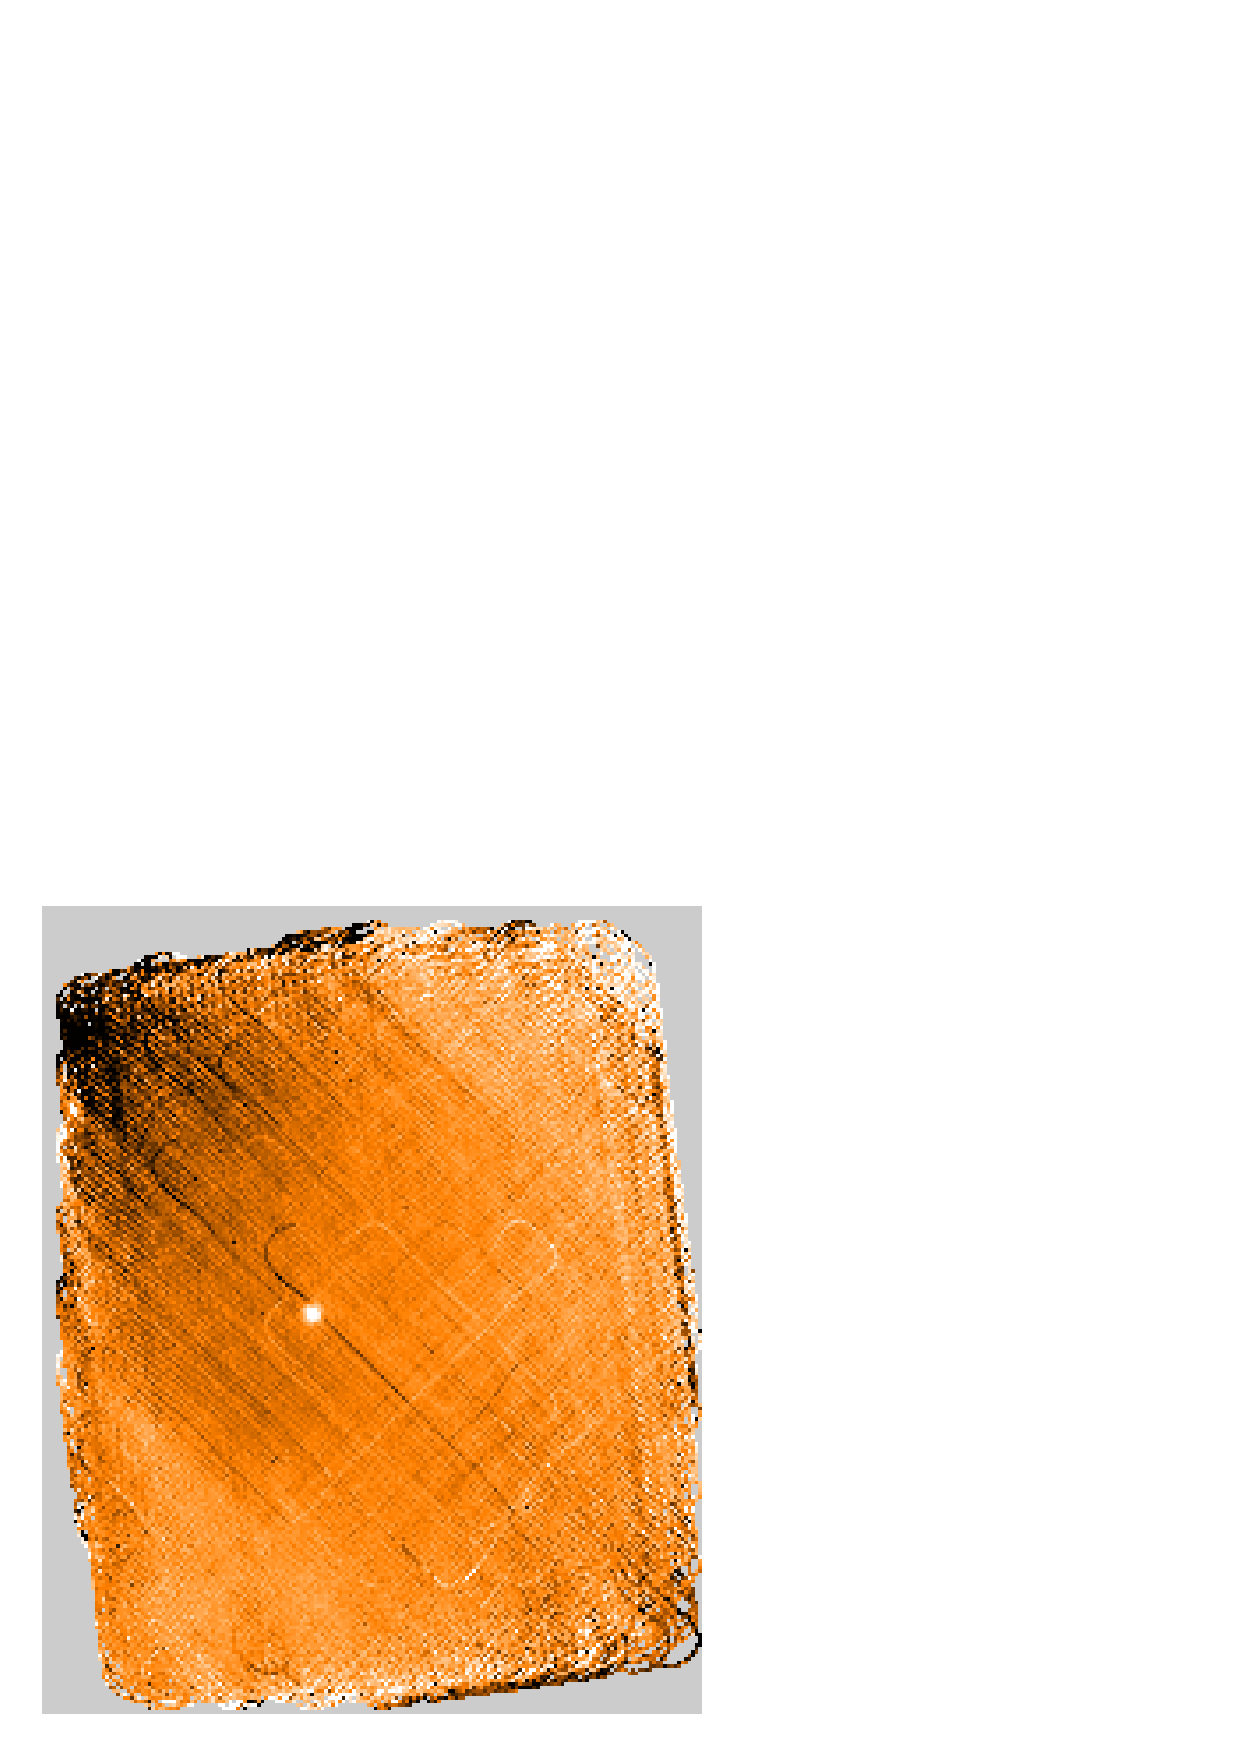
\includegraphics[width=0.5\linewidth]{sc19_map_mean_dc}
\caption{Map produced from `clean2.sdf' in which DC steps have been
  repaired and the bolometer means have been subtracted. There are
  still many artefacts in the data, but now Uranus is visible.}
\label{fig:map_dc_mean}
\end{center}
\end{figure}

The command line can get long, so it is also possible to write the
configuration parameters into a text file and specify the text file
for CONFIG using the standard group notation (`myconfig.lis' in the
following example; the leading `\verb|^|' is necessary, but it is not
part of the file name):

\begin{terminalv}
% sc2clean s4a20091214_00015_0002_con.sdf clean2 \
   config=^myconfig.lis
\end{terminalv}

An example config file containing the default values for each item
can be found in \\ \texttt{\${SMURF\_DIR}/smurf\_sc2clean.def}.

\subsubsection{\xlabel{movie}Watching a movie}

\gaia\ has the ability to animate the display of a data cube. We will
use this feature to make a `movie' of the array data. Load
`clean2.sdf' from the previous step into \gaia. In the `Display image
sections of a cube' dialogue, switch from the `Spectrum' to the
`Animation' tab approximately half-way down.  Set `Delay' to 10
milliseconds (the smallest value), `Step' to 5 (such that it only
shows 1 in every 5 frames), and click the `On' button next to
`Looping'. Finally, click `Start', and an animation of the data cube
will be shown in the main \gaia\ window. The dominant signal is a
gradual variation in the average value of all of the bolometers in
unison. This \emph{common-mode} signal is produced through a
combination of SCUBA-2 fridge temperature variations, sky noise,
telescope motion, and other drifts in the individual bolometers. At
times it is also (just barely) possible to see Uranus itself as the
array scans across is.

\subsubsection{\xlabel{fftfilter}Frequency-domain filtering}

\clean\ can also perform frequency domain filtering on the
bolometers. In the following example data are concatenated, and
filtered using a single call to \clean.

\begin{figure}
\begin{center}
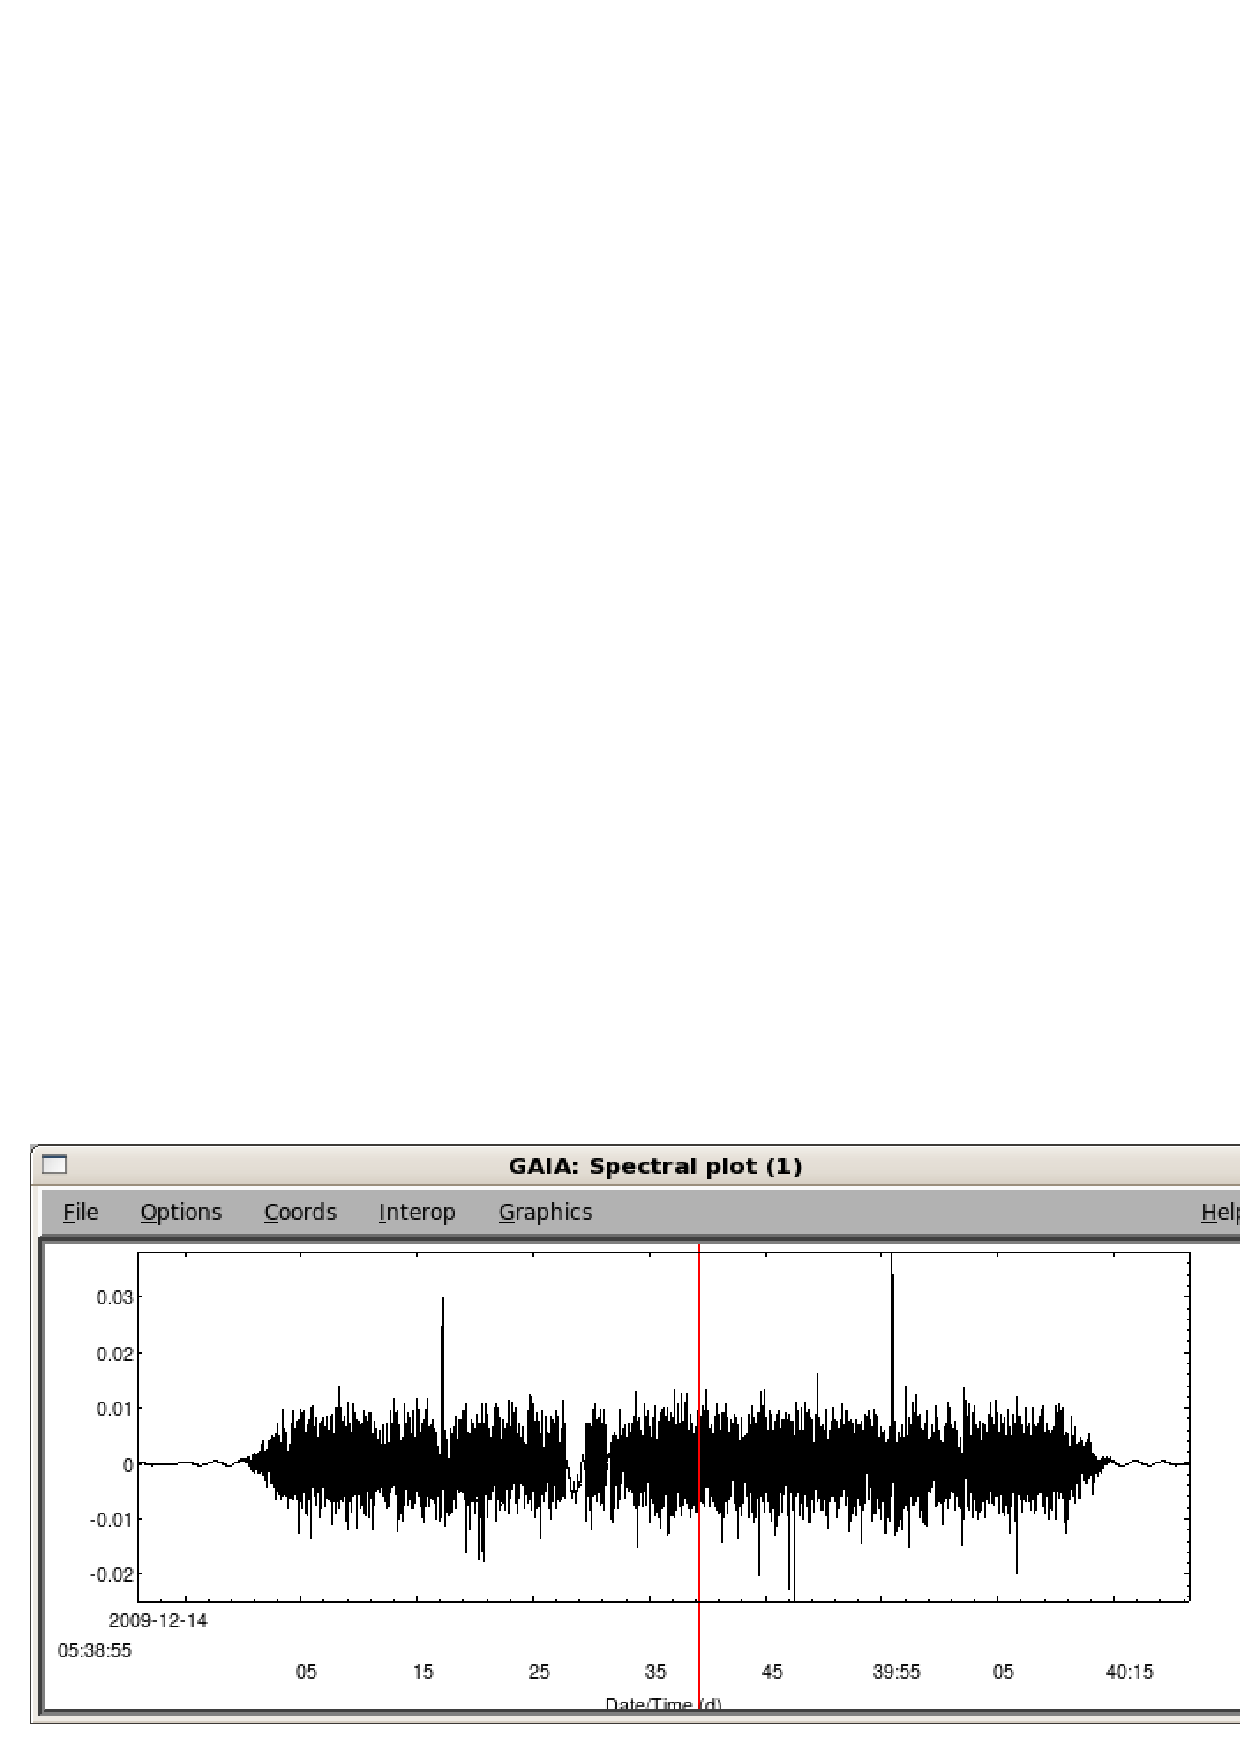
\includegraphics[width=\linewidth]{sc19_spec_filt} \\
\vspace{0.3in}
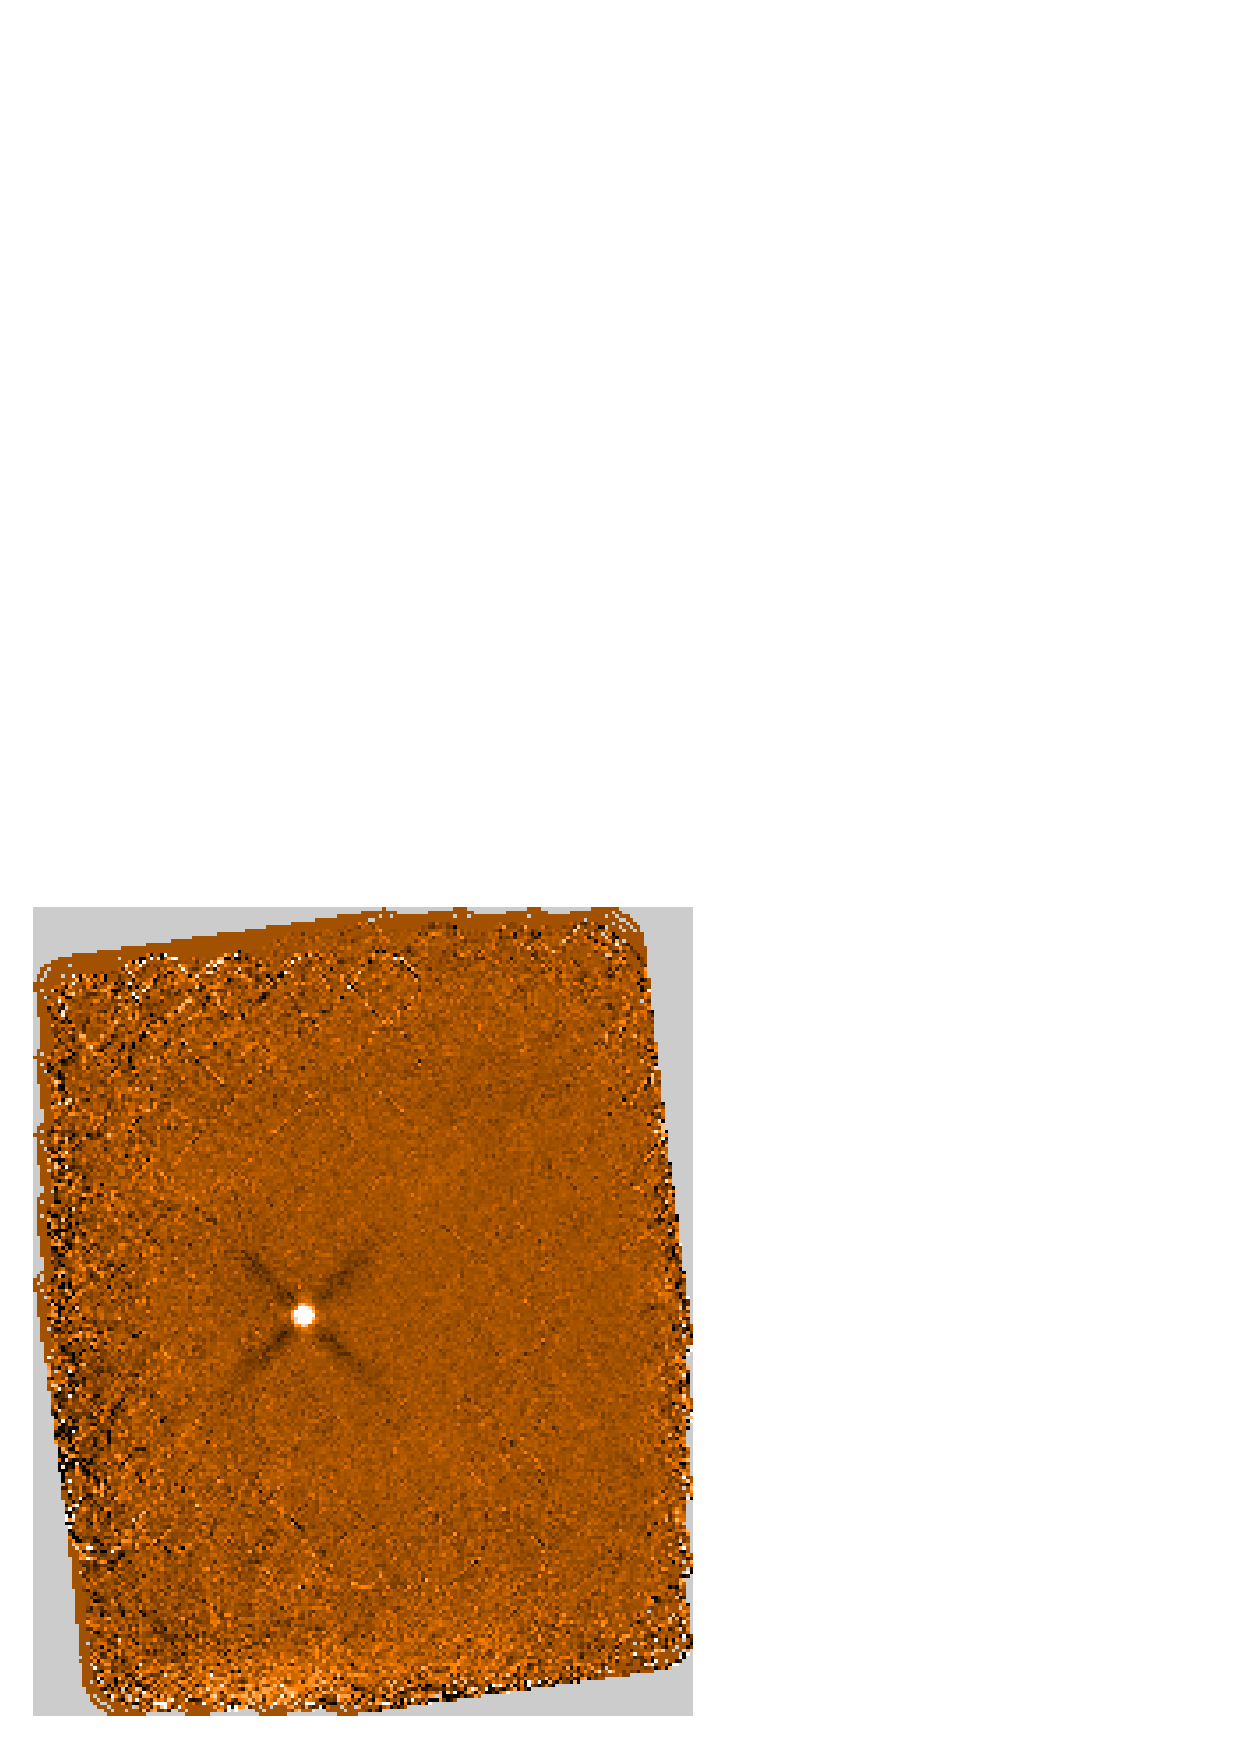
\includegraphics[width=0.5\linewidth]{sc19_map_highpass}
\caption{High-pass filtered data (clean3.sdf). \textbf{Top:} The time
  series for a single bolometer (13,23). Comparing with the un-filtered
  data in Fig.~\ref{fig:gaia_spec}, the positive spikes produced by
  Uranus are now much more apparent. \textbf{Bottom:} a map produced from
  these cleaned and filtered data. The brightness of Uranus compared
  to the noise is now much more significant than in
  Fig.~\ref{fig:map_dc_mean}, but the filtering has caused ringing
  around the source-crossing in the time series, which appears as
  negative dips in the map along the scan directions (i.e. a negative
  cross around the source).}
\label{fig:highpass}
\end{center}
\end{figure}

\begin{terminalv}
% sc2clean 's4a20091214_00015_000?.sdf' clean3 \
   config=^${STARLINK_DIR}/share/smurf/sc19_clean3.lis

Processing data from instrument 'SCUBA-2' for object 'URANUS' from the
following observation  :
  20091214 #15 scan

\end{terminalv}

Here the text file, \texttt{sc19\_clean3.lis}, contains the following
configuration options:

\begin{terminalv}
order=0
dcfitbox=30
dcthresh=25
dcsmooth=50
fillgaps=1
apod=<undef>
filt_edgehigh=0.5
\end{terminalv}

As in the early examples, the first four parameters cause \clean\ to
remove the mean bolometer values, and repair DC steps. Next, the
\texttt{apod=<undef>} (combined with an internal default
\texttt{zeropad=0}) is a slightly cryptic way to tell \clean\ to
enforce continuity between the starts and ends of each bolometer
time-series by temporarily adding padding that is a function of the
filter frequency, and interpolating the ends using a cubic
function. This step is required to avoid ringing once the FFT is
taken. The alternative, and now deprecated, method for reduing ringing
is to pad and apodize. Finally, the last parameter tells \clean\ to
apply a high-pass filter with a hard lower cutoff frequency of
0.5\,Hz.

Fig.~\ref{fig:highpass} shows the filtered bolometer signal for
(13,23), as well as a map produced from the data. The filtering has
significantly improved the noise properties of the map compared with
Fig.~\ref{fig:map_dc_mean}, but the filtering has now introduced
ringing around the source which results in a negative cross pattern
along the scan directions.

\subsection{\xlabel{pspec}Bolometer power-spectra}

The frequency-domain power spectra of SCUBA-2 bolometers can be
produced with the \smurf\ task \fft. Similar to the previous example,
we first produce cleaned, concatenated data. However, we omit the
high-pass filtering by overriding the `filt\_edgehigh' parameter
explicitly, since the goal now is to see what the full bolometer noise
power spectrum looks like.

\begin{terminalv}

% sc2clean 's4a20091214_00015_000?.sdf' clean4 \
   config="'^${STARLINK_DIR}/share/smurf/sc19_clean3.lis,filt_edgehigh=0'"

Processing data from instrument 'SCUBA-2' for object 'URANUS' from the
following observation  :
  20091214 #15 scan

% sc2fft clean4 pspec power=true

Processing data from instrument 'SCUBA-2' for object 'URANUS' from the
following observation  :
  20091214 #15 scan

Found 1 continuous chunk
SC2FFT: power spectrum requested so setting POLAR=TRUE

\end{terminalv}

While there is a \starlink\ standard format for storing complex values
as described in \cite{ssds}, \fft\ uses its own local format that
allows both for Cartesian and polar forms: a 4-dimensional array, with
the first axis indicating frequency, the second and third axes
bolometer row and column, and the final axis containing the real and
imaginary parts of each Fourier coefficient. By setting `power=true'
it switches to polar power form, such that the first element of the
4th array axis stores the square of the amplitudes, and the second
element stores the arguments (phases) of each Fourier coefficient. As
with the time series data, \gaia\ may then be used to view the data
cube. The difference is that we now specify a subset of the data so
that the 3rd axis of the cube is the array of squared Fourier
amplitudes for each bolometer, and ignore the phases (i.e.~we observe
only the 1st elements along the 4th axis):

\begin{terminalv}
% gaia 'pspec(,,,1)'
\end{terminalv}

It is then possible to click on each bolometer to display its power
spectrum. Once the `Spectral plot' window has been spawned, it will
also be necessary to modify the axis displays. Select
`Options'$\rightarrow$`Positive~Y~Only', and
`Options'$\rightarrow$`Log~Y~Axis'. Similarly, select the
corresponding settings for the `X' axis. Fig.~\ref{fig:pspec} shows
the power spectrum of bolometer (13,23), with a $1/f$ knee apparent
close to 1\,Hz.

\begin{figure}
\begin{center}
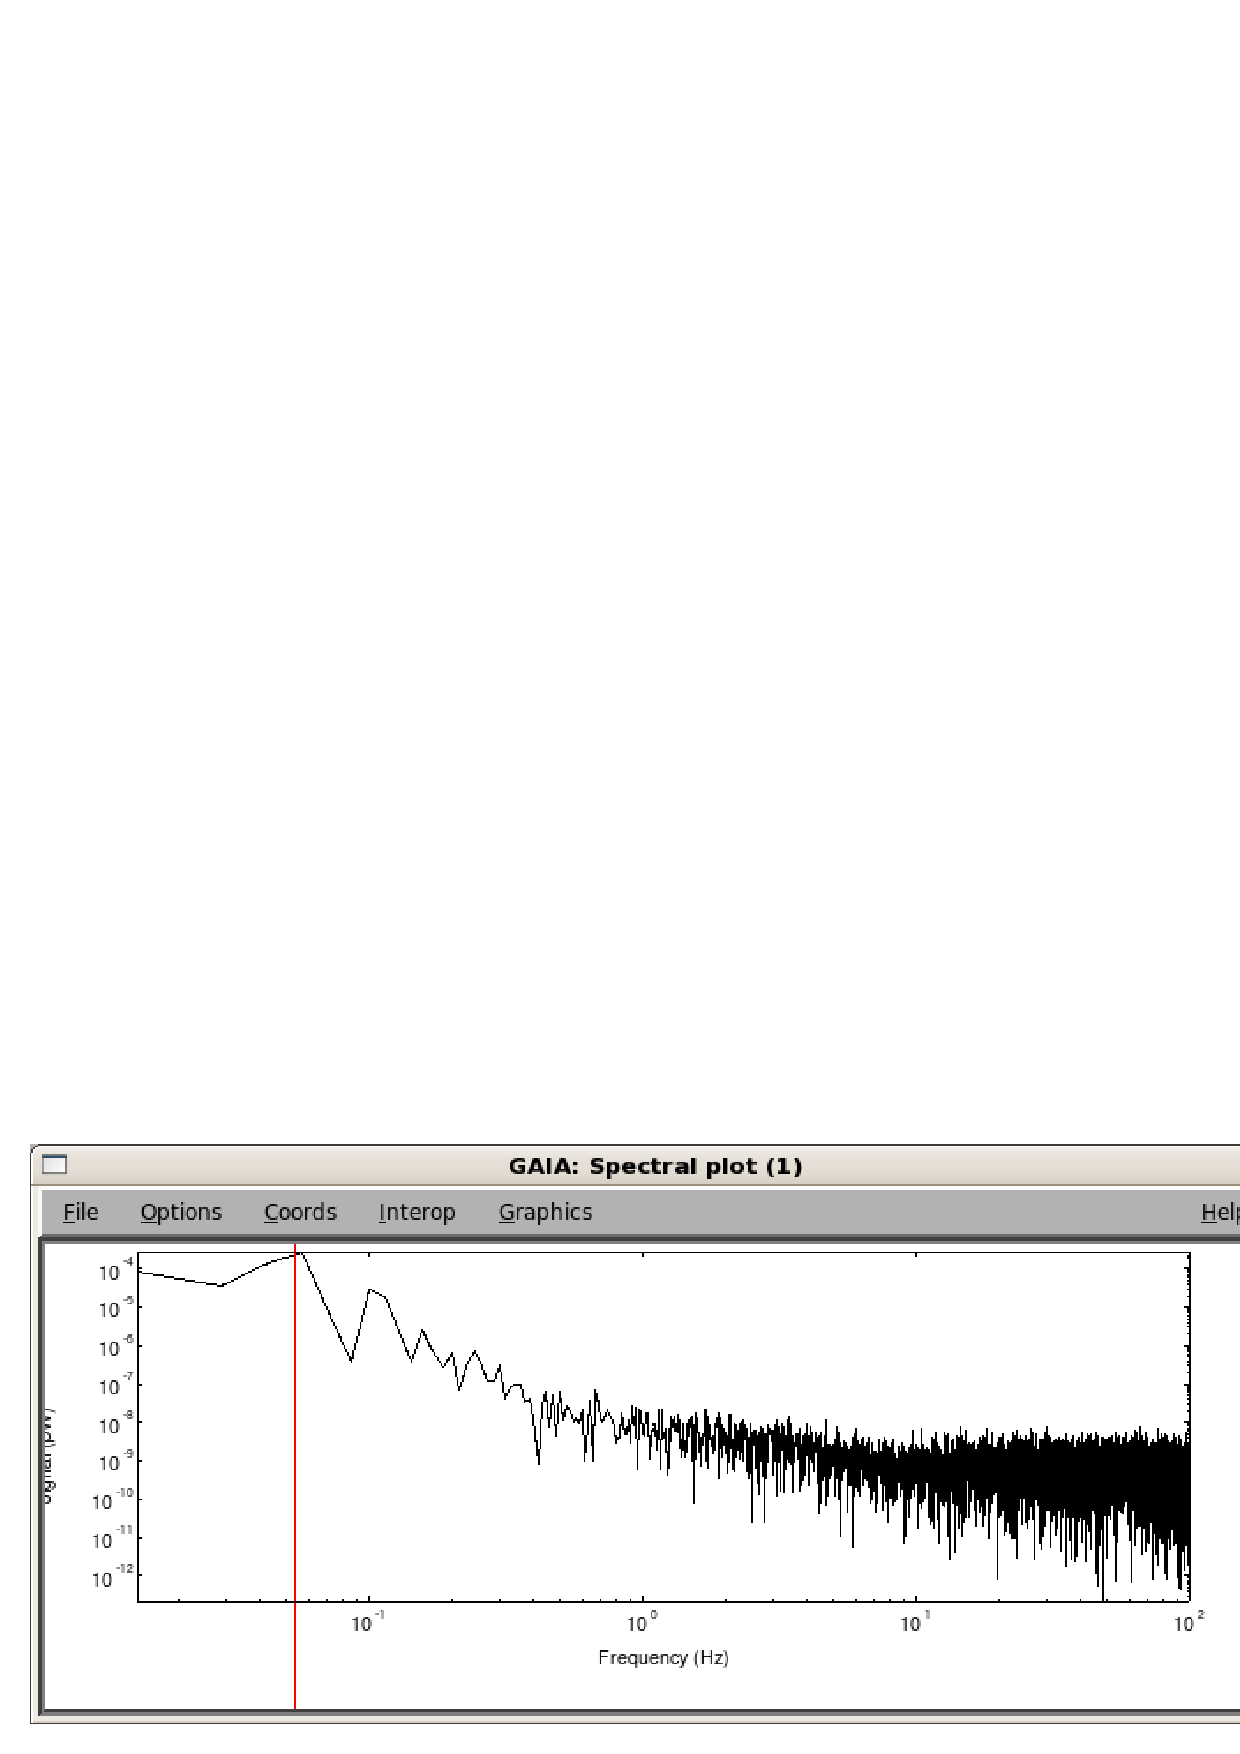
\includegraphics[width=\linewidth]{sc19_pspec}
\caption{The power spectrum of bolometer (13,23) produced by the
  \smurf\ task \fft. In this particular case the noise looks flat
  above a $1/f$ knee of about 1\,Hz. The red line simply indicates the
  frequency slice currently being displayed in the main \gaia\ window
  (not shown).}
\label{fig:pspec}
\end{center}
\end{figure}

\subsection{\xlabel{quality}Data quality flagging}
\label{sec:quality}

NDF files manipulated by \smurf\ use the standard \starlink\ named
Quality mechanism (see discussion of \xref{Masking, Bad Values, and
  Quality}{sun95}{se_masking} in \xref{SUN/95}{sun95}{}). Quality
itself is stored as an 8-bit integer for each sample in a data file,
and each bit can reflect a different condition. For example, the
following will indicate the number of samples flagged by \clean\ when
producing `clean4.sdf' in the previous example:

\begin{small}
\begin{terminalv}
% kappa


     KAPPA commands are now available -- (Version 1.13-2)

     Type kaphelp for help on KAPPA commands.
     Type 'showme sun95' to browse the hypertext documentation.

     NOTE, several applications have had major changes made to their
     parameter lists. See the 'Release Notes' section of SUN/95 for
     details.



% showqual clean4 count
  BADDA           (bit 1) - "Set iff a sample is flagged by the DA" (4416000)
  BADBOL          (bit 2) - "Set iff all data from bolo to be ignored" (4476000)
  DCJUMP          (bit 3) - "Set iff a DC jump is present" (6924)
\end{terminalv}
\end{small}

The `count' supplied to \showqual\ indicates that the total number of
occurrences of each Quality flag in the data should be counted and
displayed.  This example shows that 4416000 samples in total were
flagged `\texttt{BADDA}' by the flatfielding algorithm or by the data
acquisition (DA) system itself based on the array setup. Since each
bolometer produced 12000 samples, this corresponds to 4416000/12000
$=$ 368 bolometers that were not operational (out of 1280). The
`\texttt{BADBOL}' flag is used by \smurf\ to flag \emph{every} sample
of a bolometer that is not being used. In this case the number of
flags is 4476000 which corresponds to 373 bolometers. In other words,
cleaning turned off an additional 5 bolometers. Finally,
`\texttt{DCJUMP}' indicates the number of samples that were affected
by the DC step correction procedure (which include a number of samples
on either side of the precise locations where the steps occurred).

During map-making flagged samples will not be used and by default they
will be hidden from view for all \starlink\ tools. However, if you
wish to see the data that were flagged you can use the \Kappa\
\setbb\ command to enable a particular flag or turn them all off (so
that they can be seen in \gaia).

\begin{terminalv}
% setbb clean4 0
\end{terminalv}

will disable quality and make visible all the underlying data. Using a
value of 255 will turn all bits back on and so any non-zero quality will be
treated as bad data.

Additionally, the \Kappa\ task \qualtobad\ may be used to permanently
convert samples with given quality bits to a \emph{magic\/} or \emph{invalid\/} value. For example:

\begin{terminalv}
% qualtobad clean4 badmasked DCJUMP
\end{terminalv}
%
will set all of the samples flagged with quality \texttt{DCJUMP} to the
magic value. When `badmasked.sdf' is subsequently viewed with \gaia, none
of those portions of the data will be visible.

\section{\xlabel{maps}Dynamic Iterative Map-Making}
\label{sec:maps}

Rather than cleaning the data by hand and then re-gridding it all at
the end, we can instead do everything at once using the
\smurf\ Dynamic Iterative Map-Maker (DIMM).

The DIMM is enabled using the \texttt{method=iterate} switch to the
\makemap\ task. In the following example we will produce a map of
Uranus using the test data supplied with this \starlink\
distribution. All of the settings for the DIMM are stored in
configuration files.  In this example we will use one of the examples
that are installed in the \starlink\ tree,
`\texttt{dimmconfig.lis}'. For an overview of the different default
configuration files available see Section~\ref{sec:config}. The
parameters are also fully described in the \makemap\
documentation\footnote{See \smurfsun\ or use the \smurfhelp\ command.}
or the config files themselves. A local copy can be made and altered
if desired. The following command invokes the DIMM to produce the
image shown in Fig.~\ref{fig:itermap} with 2\,arcsec pixels:

\begin{small}
\begin{terminalv}
% makemap '$STARLINK_DIR/share/smurf/s4a20091214_00015_000?.sdf' uranus 2 \
method=iterate config=^$STARLINK_DIR/share/smurf/dimmconfig.lis

Out of 2 input files, 0 were darks, 0 were fast flats and 2 were science
Processing data from instrument 'SCUBA-2' for object 'URANUS' from the
following observation  :
  20091214 #15 scan

MAKEMAP: Map-maker will use no more than 38670 MiB of memory

   Output sky coordinates are (RA,Dec) offsets from the (moving)
   telescope base position, which started at (RA,Dec) = (23:34:38.6,
-3:33:57).

   Projection parameters used:
      CRPIX1 = 6.95327973673941e-310
      CRPIX2 = 0
      CRVAL1 = 0 ( DRA = 0:00:00.000 )
      CRVAL2 = 0 ( DDec = 0:00:00.00 )
      CDELT1 = -0.000555555555555556 ( -2 arcsec )
      CDELT2 = 0.000555555555555556 ( 2 arcsec )
      CROTA2 = 0

   Output map pixel bounds: ( -74:112, -113:116 )

   Output map WCS bounds:
        Right ascension offset: -0:00:14.867 -> 0:00:10.067
        Declination offset: -0:03:49.00 -> 0:03:51.00

smf_iteratemap: Iterate to convergence (max 5)
smf_iteratemap: Stopping criteria is a change in chi^2 < 0.001
smf_iteratemap: map-making requires 1355 MiB (map=1 MiB model calc=1353 MiB)
smf_iteratemap: Continuous chunk 1 / 1 =========
smf_iteratemap: Iteration 1 / 5 ---------------
--- Size of the entire data array ------------------------------------------
bolos  : 1280
tslices: bnd:0(0.0 min), map:12000(1.4 min), tot:12000(1.4 min)
Total samples: 15360000
--- Quality flagging statistics --------------------------------------------
 BADDA:    4416000 (28.75%),         368 bolos
BADBOL:    4956000 (32.27%),         413 bolos
DCJUMP:       1557 ( 0.01%),
 NOISE:     480000 ( 3.12%),          40 bolos
Total samples available for map:   10402995, 67.73% of max (866.916 bolos)
smf_iteratemap: Calculate time-stream model components
smf_iteratemap: Rebin residual to estimate MAP
smf_iteratemap: Will calculate chi^2 next iteration
smf_iteratemap: Calculate ast
--- Quality flagging statistics --------------------------------------------
 BADDA:    4416000 (28.75%),         368 bolos  ,change          0 (+0.00%)
BADBOL:    5292000 (34.45%),         441 bolos  ,change     336000 (+6.78%)
 SPIKE:        137 ( 0.00%),                    ,change        137 (+inf%)
DCJUMP:       1557 ( 0.01%),                    ,change          0 (+0.00%)
   COM:     369162 ( 2.40%),                    ,change     369162 (+inf%)
 NOISE:     480000 ( 3.12%),          40 bolos  ,change          0 (+0.00%)
Total samples available for map:   10033706, 65.32% of max (836.142 bolos)
     Change from last report:    -369289, -3.55% of previous
smf_iteratemap: Iteration 2 / 5 ---------------
smf_iteratemap: Calculate time-stream model components
smf_iteratemap: Rebin residual to estimate MAP
smf_iteratemap: *** CHISQUARED = 1.15486085552371 for filegroup 1

\end{terminalv}
\end{small}

This excerpt shows the initial output of the DIMM. Note that the basic
dimensions of the data being processed are listed near the start of
the first iteration, as well as the QUALITY flagging statistics. This
report is similar to that produced by the \Kappa\ task \showqual\ in
Section~\ref{sec:quality}. At the beginning, the main purpose is to
indicate how many bolometers are being used: 368 bolometers were
turned off during data acquisition (\texttt{BADDA}); and 40 bolometers
exceeded the acceptable noise threshold (\texttt{NOISE}). There were
also small numbers of samples flagged as containing spikes and
jumps. The total number of bad bolometers (\texttt{BADBOL}) is
413. Accounting for these, and the small numbers of additionally
flagged samples, $866.916$ effective bolometers are available at the
start of the first iteration.

After each subsequent iteration a new QUALITY report is produced,
indicating how the flags have changed. An important flag that appears
in the QUALITY report following the first iteration is \texttt{COM}:
the DIMM rejects bolometers (or portions of their time series) if they
differ significantly from the common-mode (average) of the remaining
bolometers. Another useful quantity reported is \texttt{CHISQUARED} --
the RMS of the residual (time series with the various model components
removed) for all of the samples with good QUALITY, normalized by the
measured white noise levels.

This particular configuration executes a maximum of 5 iterations, but
stops sooner if the change in \texttt{CHISQUARED} is less then
0.001. In this case, it reaches this stopping criterion after 5
iterations:

\begin{small}
\begin{terminalv}
smf_iteratemap: Iteration 5 / 5 ---------------
smf_iteratemap: Calculate time-stream model components
smf_iteratemap: Rebin residual to estimate MAP
smf_iteratemap: *** CHISQUARED = 1.14451425189281 for filegroup 1
smf_iteratemap: *** change: -2.48779013769518e-05
smf_iteratemap: Calculate ast
--- Quality flagging statistics --------------------------------------------
 BADDA:    4416000 (28.75%),         368 bolos  ,change          0 (+0.00%)
BADBOL:    5304000 (34.53%),         442 bolos  ,change          0 (+0.00%)
 SPIKE:        180 ( 0.00%),                    ,change          0 (+0.00%)
DCJUMP:       1557 ( 0.01%),                    ,change          0 (+0.00%)
   COM:     392350 ( 2.55%),                    ,change       1670 (+0.43%)
 NOISE:     480000 ( 3.12%),          40 bolos  ,change          0 (+0.00%)
Total samples available for map:   10010475, 65.17% of max (834.206 bolos)
     Change from last report:      -1670, -0.02% of previous
smf_iteratemap: ****** Completed in 5 iterations
smf_iteratemap: ****** Solution CONVERGED
Total samples available from all chunks: 10010475 (834.206 bolos)
\end{terminalv}
\end{small}

Note that compared to the initial report, the total number of samples
with good QUALITY (\texttt{Total samples available for map}) has
dropped from 10402995 to 10010475 (about a 4 per cent decrease) as
additional samples were flagged in each iteration.

\begin{figure}
\begin{center}
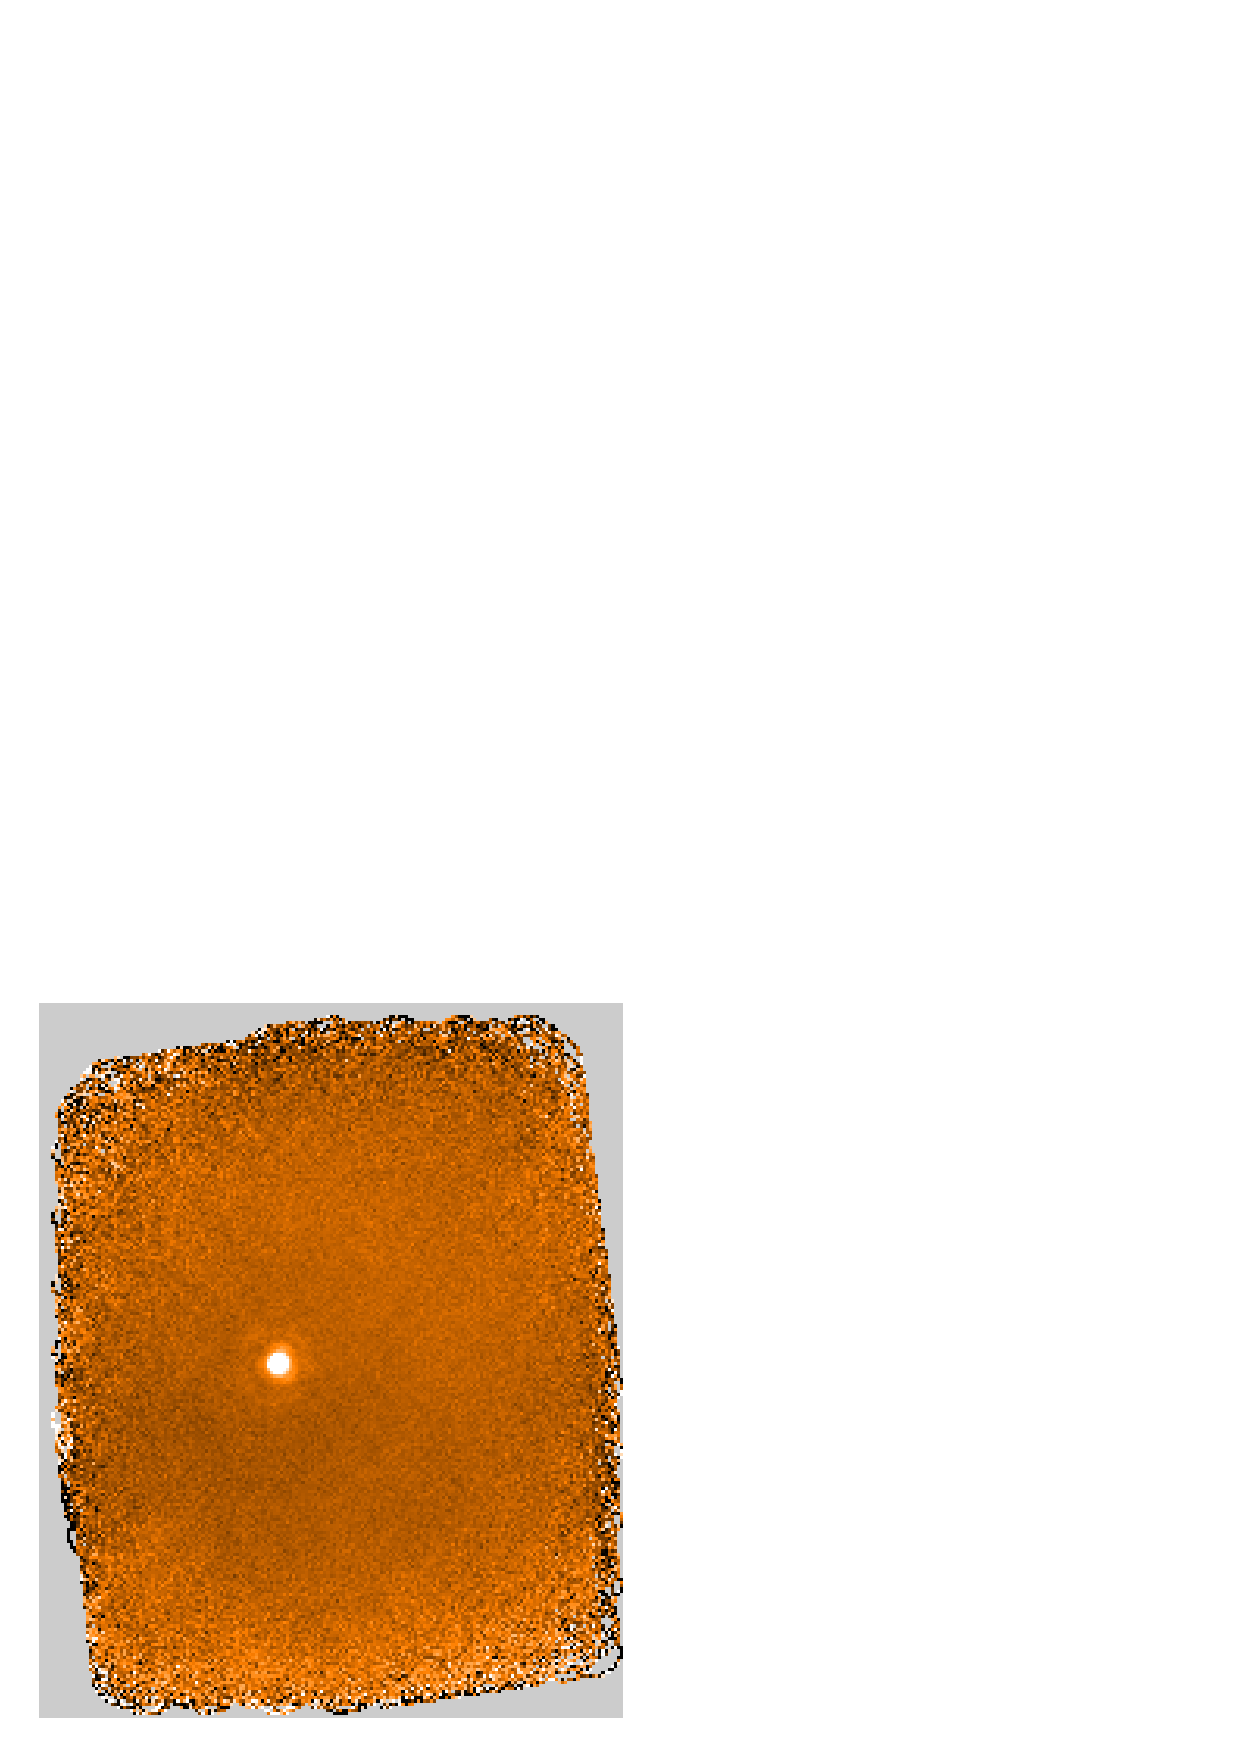
\includegraphics[width=0.5\linewidth]{sc19_map_iterate}
\caption{Map of Uranus produced with the \smurf\ task \makemap\ using
  the iterative algorithm with default parameters. The S/N of the
  source is now greatly improved compared to the simplistic reduction
  in Fig.~\ref{fig:highpass}, and the negative ringing has been
  removed.}
\label{fig:itermap}
\end{center}
\end{figure}

The iterative map-maker estimates several components of the bolometer
signal in addition to the astronomical signal that goes into the
map. The particular sequence of components that it fits is specified
by \texttt{modelorder} in the configuration file. All of the examples
provided with \smurf\ are derived from
\texttt{\$STARLINK\_DIR/share/smurf/dimmconfig.lis}, and we show the
relevant excerpt here:

\begin{terminalv}
# Model components/order (comma separated list in brackets)
# Note: components specified AFTER 'ast' will not be calculated for the
# first time until the second iteration.
#  dks = fit and remove dark squid for the column
#  com = remove common-mode signal
#  gai = if com specified, fit gain/offset of common mode
#  ext = apply extinction correction
#  ast = estimate the map and astronomical signal
#  flt = apply filter to time streams
#  noi = estimate time-domain variance
#  smo = time series smoothing using a median or mean boxcar filter
#  pln = remove plane from each time slice

modelorder = (com,gai,ext,flt,ast,noi)
\end{terminalv}

By default, the final values of these fitted models are \emph{not}
written to files. However, this can be modified by setting
\texttt{exportndf} in the configuration file to the list of models
that you wish to view:

\begin{terminalv}
# Specify a value of 1 or 0 to export all or none of the components
# You can also specify an array of components to export using the same
# format as modelorder. Note that you can specify additional
# components 'res' and 'qua' to what may be provided to modelorder if
# you wish to export the residual model or quality arrays
# respectively. Exportation of 'res' is implied if 'noi' is specified
# as it becomes the variance components of the resulting NDF for
# 'res'. 'qua' will become the quality component of any full 3-dimensional
# model (e.g. 'res', 'ast', 'flt', 'ext'), but no quality will be
# written to model components with different dimensions.

exportndf = (com,gai,ast,flt,res,noi,qua)
\end{terminalv}

If we make a local copy of \texttt{dimmconfig.lis}, add the above
\texttt{exportndf} line, and re-run the iterative map-maker with this
modified configuration, it now produces several new files at the end:

\begin{terminalv}
s4a20091214_00015_0002_con_ast.sdf
s4a20091214_00015_0002_con_com.sdf
s4a20091214_00015_0002_con_gai.sdf
s4a20091214_00015_0002_con_flt.sdf
s4a20091214_00015_0002_con_res.sdf
\end{terminalv}

Note that the quality and variance for the data are stored as the
VARIANCE and QUALITY components within the residual file NDF.

As with the input data, these are all standard \starlink\ NDF files
which can be examined using all of the existing tools, and can be used
by other \smurf\ routines such as \clean, \fft, and \makemap. The base
of the filenames is the first input file that went into the maps for
each subarray, and the `\texttt{con}' suffix indicates that several
data files may have been concatenated together. The new files are:
`\texttt{*ast.sdf}', the time-domain projection of the astronomical
signal as estimated in the final map (same dimensions as the input
bolometer data); `\texttt{*com.sdf}', an estimate of the common-mode
signal (predominantly sky emission and fridge temperature variations);
`\texttt{*flt.sdf}', additional noise (low-frequency noise in this
particular case) that was filtered out of each bolometer (same
dimensions as the input bolometer data); and finally
`\texttt{*res.sdf}', the residual bolometer signal once the other
components have been subtracted from the original data, which should
look predominantly like white noise (again, same dimensions as the
input bolometer data).

\begin{figure}
\begin{center}
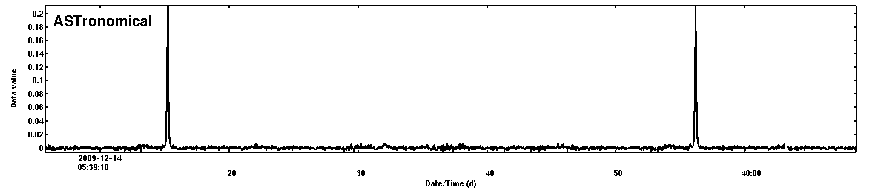
\includegraphics[width=\linewidth]{sc19_iter_ast} \\
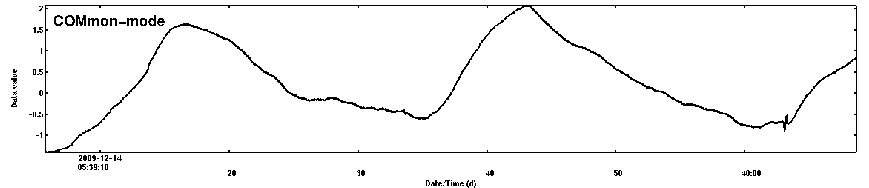
\includegraphics[width=\linewidth]{sc19_iter_com} \\
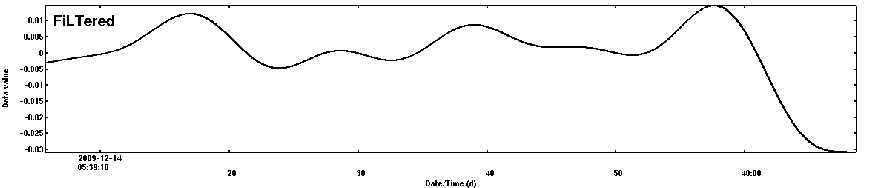
\includegraphics[width=\linewidth]{sc19_iter_flt} \\
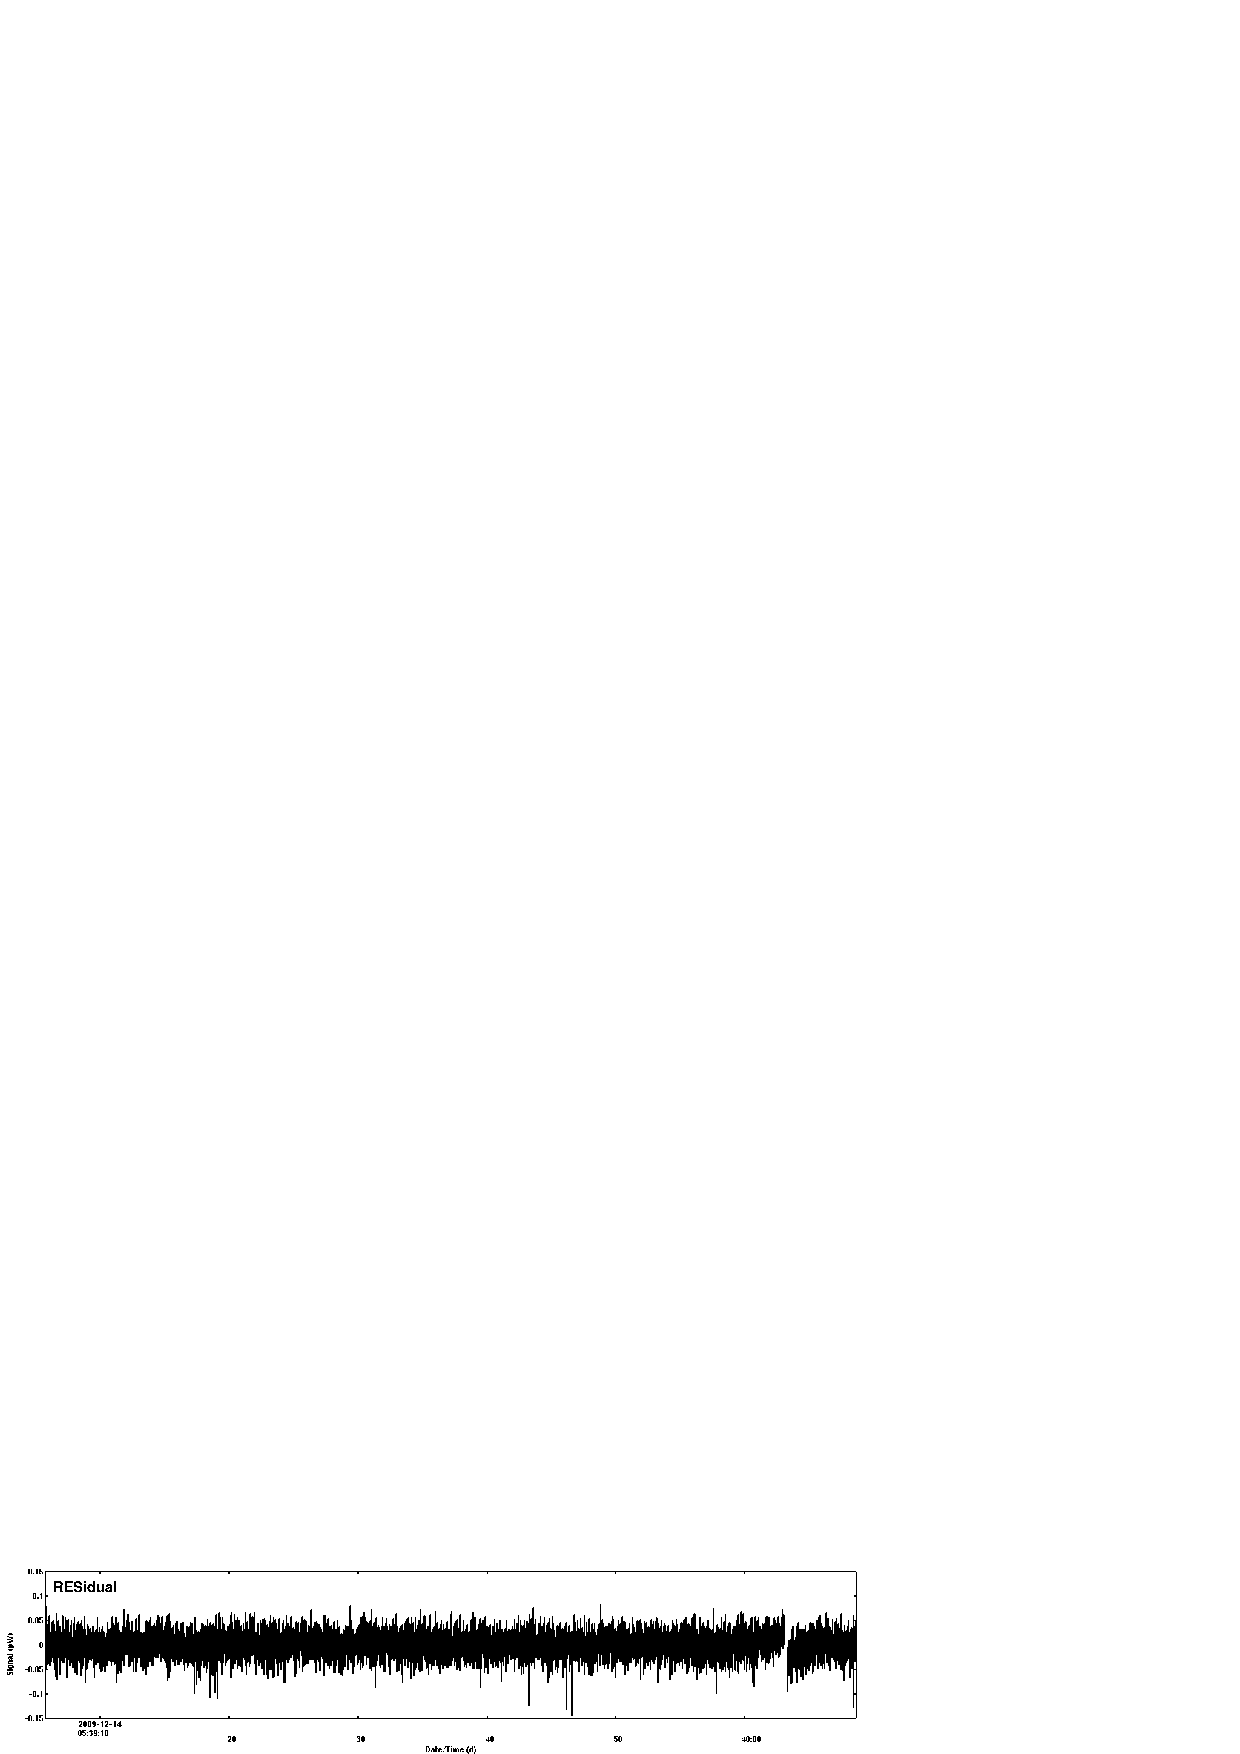
\includegraphics[width=\linewidth]{sc19_iter_res} \\
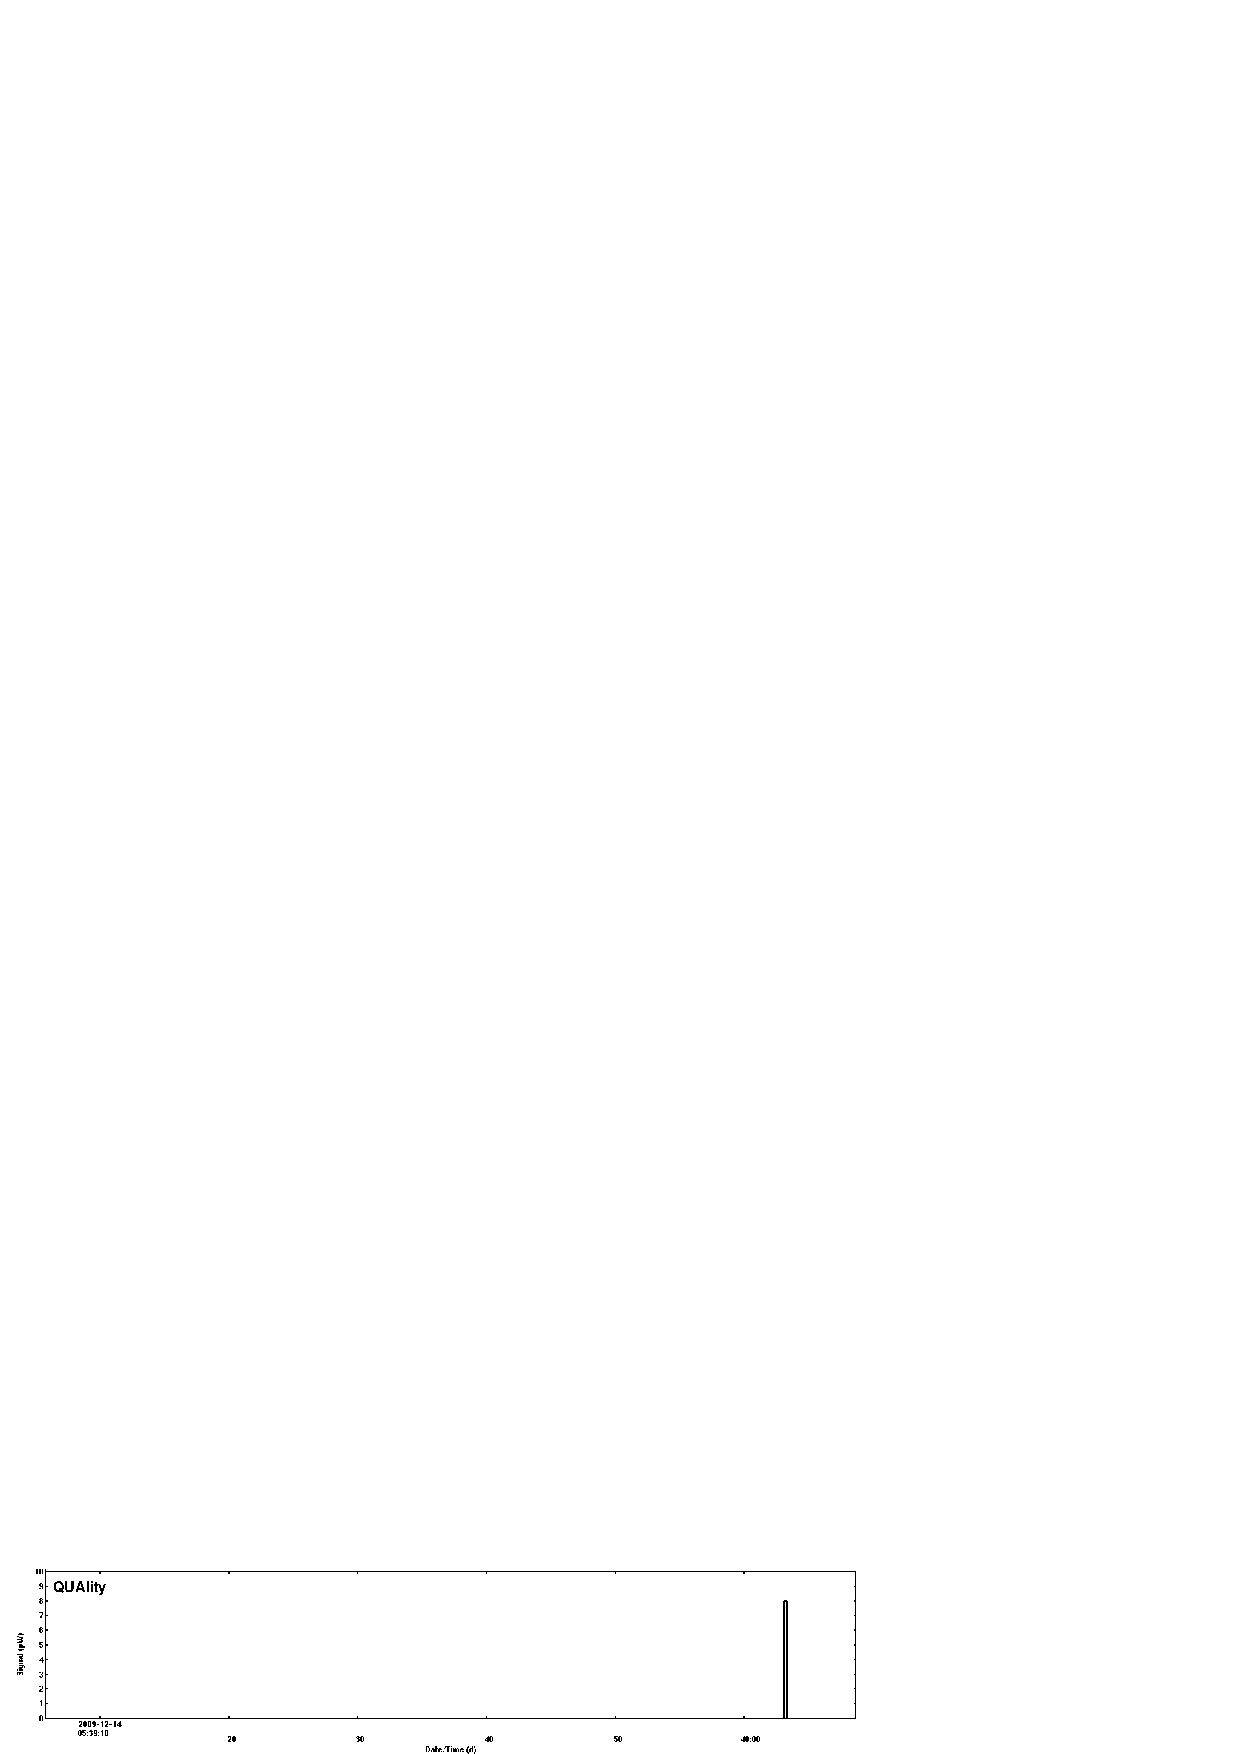
\includegraphics[width=\linewidth]{sc19_iter_qua} \\
\caption{Time-domain components of the iterative solution for
  bolometer (13,23). From top to bottom: ASTronomical signal (clearly
  showing Uranus as positive spikes); COMmon mode (dominated by 30\,s
  fridge variations); FiLTered (residual low-frequency noise missed by
  COM); RESidual (looking flat, except for a small residual around the
  location of a repaired DC step); and QUAlity (indicating the
  location of the DC step -- the numerical value 8; this region of the
  data is not used in the final map). All of the plots were produced
  with \gaia, restricting the range of the $x$-axis to samples
  2840--11500.}
\label{fig:itercomp}
\end{center}
\end{figure}

Time traces for a single bolometer are compared for all of these model
components in Fig.~\ref{fig:itercomp}. Uranus is clearly seen as a
positive spike in the astronomical signal component. The common-mode
signal is the next largest, clearly exhibiting the 30\,s fridge
variations that are apparent in the raw data. The residual noise
removed by the high-pass filter is significant, but much smaller than
the common-mode component. Finally, the residual signal is quite flat,
indicating that most of the signal has been accounted for in the other
model components.

\subsection{\xlabel{config}Configuration Files}
\label{sec:config}

Since the DIMM has a large number of parameters, several configuration
files are supplied with \smurf\ for reducing common types of data. All
of these files can be found in
\\ \texttt{\$STARLINK\_DIR/share/smurf/} with filenames of the form
\texttt{dimmconfig*.lis}. The default \texttt{dimmconfig.lis} should
give reasonable results for most observations. Note that this file
also contains the full set of parameters with extensive
documentation. For clarity, all of the other configuration files for
specific observations types are derived from \texttt{dimmconfig.lis}
and simply override the relevant parameters.

While we have tested a wide variety of data sets with these files, it
is certainly worth trying at least the default, and the specific
configuration that sounds like it would be appropriate for your
project:

\begin{description}

\item[\texttt{dimmconfig.lis}]\quad Before the iterative solution
  begins, some pre-processing steps are performed, like repairing DC
  steps, turning off particularly noisy bolometers (see the
  \\ \texttt{noiseclip} parameter), and the mean levels are
  subtracted.  This default configuration solves for the following
  models: \texttt{COM}, \texttt{GAI}, \texttt{EXT}, \texttt{FLT},
  \texttt{AST}, \texttt{NOI}. The components \texttt{COM} and
  \texttt{GAI} work together to calculate the average signal template
  of all the bolometers, and then fit/remove the templates from each
  bolometer. They also identify outlier bolometers that do not
  resemble the template and remove them from the final solution. The
  component \texttt{EXT} applies the extinction correction (derived
  from the water-vapour radiometer by default), and then \texttt{FLT}
  applies a high-pass filter to the data, above frequencies that
  correspond to angular scales of 600\,arcsec and 300\,arcsec at
  450\micron\ and 850\micron, respectively (as established
  automatically from the mean slew speed of the scan). These cutoff
  frequencies were chosen through trial and error, but appear to give
  good results under a wide variety of situations. Finally,
  \texttt{AST} estimates the astronomical signal contribution to the
  bolometer signals from the current map estimate, and \texttt{NOI}
  measures the noise in the residual signals for each bolometer to
  establish weights for the data as they are placed into the map in
  subsequent iterations.

\item[\texttt{dimmconfig\_blank\_field.lis}]\quad This configuration
  is tuned for deep surveys for which the goal is to detect low-S/N
  point sources. Instead of iteratively applying a high-pass filter
  (\texttt{FLT}), which can result in convergence problems when there
  is little signal in the map, a single, harsher high-pass filter is
  applied as a pre-processing step (corresponding to 200\,arcsec
  scales at both 450\micron\ and 850\micron). There are also more
  conservative cuts to remove noisy/problematic bolometers. Finally,
  the parameters \texttt{ast.zero\_lowhits} and
  \texttt{ast.zero\_notlast} are set to constrain much of the map to
  precisely zero for all but the last of 5 iterations. This helps with
  map convergence, and is a reasonable prior for a
  blank-field. Normally the map would then be processed using a
  matched filter (see Section~\ref{sec:cosmology}).

\item[\texttt{dimmconfig\_bright.lis}]\quad This configuration is
  aimed at reducing maps of bright sources. Weaker noise clipping, DC
  step thresholds and common-mode rejection are used. In addition, the
  number of iterations is increased to a fixed value of 20 to allow
  potentially large-scale structures to converge.

\item[\texttt{dimmconfig\_bright\_compact.lis}]\quad This
  configuration is aimed at reducing maps of bright, compact sources
  that are isolated at the centre of the map, and is derived from
  \texttt{dimmconfig\_bright.lis}. The addition of
  \texttt{ast.zero\_circle} and \texttt{ast.zero\_notlast} parameters
  are used to constrain the map to zero beyond a radius of 1\,arcmin
  for all but the final iteration. This strategy helps with map
  convergence significantly, and can provide good maps of bright
  sources, even in cases where scan patterns failed and the telescope
  degenerated into scanning back-and-forth along a single position
  angle on the sky.

\item[\texttt{dimmconfig\_bright\_extended.lis}]\quad This
  configuration is for reducing maps of bright extended sources, and
  is also derived from \texttt{dimmconfig\_bright.lis}. Here
  \texttt{ast.zero\_snr} is used to constrain the map to zero wherever
  the S/N is lower than 5-$\sigma$. We recommend setting the parameter
  \texttt{itermap=1}, and then visually inspecting the maps produced
  after each iteration (e.g., \texttt{gaia map.more.smurf.itermaps})
  to help determine an appropriate number of iterations.

%\item[\texttt{dimmconfig\_distortionmap.lis}] This configuration is
%  used primarily by the instrument team to produce single bolometer
%  maps for finely-spaced scans over calibrators (see the
%  \texttt{bolomap} parameter). These are used to measure the
%  focal-plane offsets for each bolometer, and to constrain the relative
%  bolometer responsivities.

%\item[\texttt{dimmconfig\_faint\_extended.lis}]\quad It is presently
%  very challenging to produce SCUBA-2 maps of faint extended
%  structures, given the instrument's low-frequency noise
%  performance. In particular, for some observing configurations, wide
%  scans can suffer significant magnetic field pickup. If there are no
%  bright sources in the map, a single high-pass filter may be applied
%  at the start (as in \texttt{dimmconfig\_blank\_field.lis}). Then,
%  the dark-squid signals (one for each column in the array, sensitive
%  primarily to this pickup) can be used as templates to fit and remove
%  this extra low-frequency noise component, the \texttt{DKS}
%  model. Note that for maps of brighter structures, \texttt{DKS} does
%  not have much of an impact, and may simply increase the noise, as
%  all three of \texttt{COM}, \texttt{FLT}, and \texttt{DKS} model the
%  low-frequency bolometer noise, and are somewhat degenerate.  In
%  addition, a more conservative cut on noisy bolometers is applied
%  (\texttt{noiseclip=2.0}).

%\item[\texttt{dimmconfig\_veryshort.lis}]\quad Some scans of
%  calibrators for the purpose of focus or pointing are extremely short
%  (e.g.~10\,s). In these cases it makes no sense to pad and apodize in
%  order to filter out noise on time scales comparable to, or longer
%  than the entire scan. This configuration turns off apodization and
%  the \texttt{FLT} model, relying only on the mean subtraction and
%  \texttt{COM} to model and remove the low-frequency noise.

%\item[\texttt{dimmconfig\_fridgeflat.lis}] This configuration is also
%  primarily for use by the engineering team. It was designed to reduce
%  data with the SCUBA-2 shutter closed, in order to study the response
%  of the bolometers to internal temperature variations in the
%  refrigeration system.

%\item[\texttt{dimmconfig\_newfilt.lis}] This configuration file
%  illustrates an alternative method for handling gaps in the data. By
%  default, when portions of a bolometer data stream are flagged, they
%  are filled with a constrained realisation of noise to ensure
%  continuity when filtering (although the samples themselves are not
%  added to the final map). This modified configuration handles the
%  problem of gaps by creating a window function with `1' at locations
%  of good data, and `0' where there are gaps. Both the real data (with
%  gaps) and this window function are filtered. The ringing in the
%  filtered window function can then be used to compensate for ringing
%  in the real filtered data caused by the gaps. This method can
%  preserve more of the data, and is probably more robust. However, it
%  requires more memory and is slightly slower, and gives results that
%  closely resemble the defaults.

\end{description}

If you want to modify parameters for a particular config file the best
approach is to create a new file and first include a directive to load
the file you want to modify and then supply your own parameters. You
can see this technique is used in the installed configuration files to
reference them all to \texttt{dimmconfig.lis}.

\section{\xlabel{calib}Calibrating SCUBA-2 Data}
\label{sec:calib}

\subsection{\xlabel{extinction}Extinction Correction}

Analysis of the SCUBA-2 skydips and heater-tracking data from the
S2SRO data has allowed calculation of the opacity factors for the
SCUBA-2 450\micron\ and 850\micron\ filters to be determined. Full
details of the analysis and on-sky calibration methods of SCUBA-2 can
be found in Dempsey et al.\ (2010)~\cite{dempsey-spie}.

Archibald et al. (2002)~\cite{archibald} describes how the
Caltech Submillimeter Observatory (CSO) 225\,GHz opacity,
$\tau_{225}$, relates to SCUBA opacity terms in each band,
$\tau_{450}$ and $\tau_{850}$. It was assumed for commissioning and
S2SRO that the new SCUBA-2 filters are sufficiently similar to the
wide-band SCUBA filters that these terms could be used for extinction
correction. In the form $\tau_{\lambda} = a \times (\tau_{225} - b)$,
the original SCUBA corrections were:
\begin{equation}
\tau_{450} = 26.2 \times (\tau_{225} - 0.014);
\end{equation}
and
\begin{equation}
\tau_{850} = 4.02 \times (\tau_{225} - 0.001).
\end{equation}

The JCMT water-vapour radiometer (WVM) is now calibrated to provide a
higher-frequency opacity value which has been scaled to
$\tau_{225}$. The WVM (not the CSO 225\,GHz tipper) data were used for
this analysis.

The new filter opacities as determined from skydip data are as
follows:

\begin{equation}
\tau_{450} = 19.04 \times (\tau_{225} - 0.018);
\end{equation}
and
\begin{equation}
\tau_{850} = 5.36 \times (\tau_{225} - 0.006).
\end{equation}

The SCUBA-2 filters are different from the SCUBA filters, with the
450\micron\ filter, in particular, significantly narrower than its
SCUBA counterpart. The SCUBA-2 filter characteristics are described in
detail \htmladdnormallinkfoot{on the JCMT
  website}{http://www.eaobservatory.org/jcmt/instrumentation/continuum/scuba-2/filters/}.

The extinction correction parameters that scale from $\tau_{225}$ to
the relevant filter have been added to the map-maker code. You can
override these values by setting \param{ext.taurelation.filtname} in
your map-maker config files to the three coefficients `(a,b,c)' that you
want to use (where `\texttt{filtname}' is the name of the filter). The
defaults are listed in \texttt{\$SMURF\_DIR/smurf\_extinction.def}. We have
also added a slight calibration tweak to WVM-derived values to correct
them to the CSO scale. It is worth noting that if an individual
science map and corresponding calibrator observation has already been
reduced with the old factors (and your source and calibrator are at
about the same airmass and if the tau did not change appreciably), any
errors in extinction correction should cancel out in the calibration.


\subsection{\xlabel{fcf}Flux conversion factors}
\label{sec:fcf}

Primary and secondary calibrator observations have been reduced using
the specifically designed
\texttt{dimmconfig\_bright\_compact.lis}. The maps produced from this
are then analysed using tailor-made \picard\ recipes. \picard\ is a
post-processing and data combination tool that uses the same
infrastructure as ORAC-DR, but is designed to be used after the
initial reduction with the DIMM is complete. Details of the \picard\
recipes and how to use them can be found on \htmladdnormallinkfoot{the
  ORAC-DR web page}{http://www.oracdr.org/oracdr/PICARD}.

A map reduced by the mapmaker has units of pW. To calibrate the data
into units of janskys (Jy), a set of bright, point-source objects with
well known flux densities are observed regularly to provide a flux
conversion factor (FCF). The data (pW) can be multiplied by this FCF
to obtain a calibrated map, and the FCF can also be used to assess the
relative performance of the instrument from night to night. The noise
equivalent flux density (NEFD) is a measure of the instrument
sensitivity, and while not discussed here, is also produced by the
\picard\ recipe shown here. For calibration of primary and secondary
calibrators, the FCFs and NEFDs have been calculated as follows:
\begin{enumerate}
\item{The \picard\ recipe \drrecipe{SCUBA2\_FCFNEFD} takes the reduced
  map, crops it, and runs background removal. Surface fitting
  parameters are changeable in the \picard\ parameter file.}
\item{It then runs the \Kappa\ \beamfit\ task on the specified point
  source. The \beamfit\ task will estimate the peak (uncalibrated)
  flux density and the FWHM. The integrated flux density within a
  given aperture (30\,arcsec radius default) is calculated using
  \photom\ \autophotom. Flux densities for calibrators such as Uranus,
  Mars, CRL\,618, CRL\,2688 and HL\,Tau are already known to
  \picard. To derive an FCF for other sources of known flux densities,
  the fluxes can be added to the parameter file with the source name
  (in upper case, spaces removed): \texttt{FLUX\_450.MYSRC = 0.050}
  and \texttt{FLUX\_850.MYSRC = 0.005} (where the values are in Jy),
  for example. }

  An example of a \picard\ parameter file (used for reduction of the
  850\micron\ calibrators) is shown here:

\begin{terminalv}
[SCUBA2_FCFNEFD]
APERTURE_RADIUS=30.0
AUTOPHOTOM=1
MASK_SOURCE=1
BACKGROUND_FITMETHOD=fitsurface
FITSURFACE_FITTYPE=spline
FITSURFACE_FITPAR=4
USEFCF=1
FLUX_850.ARP220=0.688
FLUX_850.ALPHAORI=0.629
FLUX_850.TWHYDRAE=1.37
FLUX_850.V883ORI=1.34
LOGFILE=1
\end{terminalv}

\item {It then uses the above procedure to calculate the three
  alternative FCF values described below.}
\end{enumerate}

\begin{itemize}

\item{\textbf{\fcfa} (surface brightness calibration)}

\begin{equation}
\label{eq:fcf_arcsec}
\mathrm{FCF_{arcsec}} = \frac{S_\mathrm{tot}}{P_\mathrm{int} \times
  A_\mathrm{pix}},
\end{equation}

where $S_\mathrm{tot}$ is the total flux density of the calibrator,
$P_\mathrm{int}$ is the integrated sum of the source in the map (in
pW) and $A_\mathrm{pix}$ is the pixel area in arcsec$^2$, producing an
FCF in Jy/arcsec$^2$/pW. This \fcfa\ is the number to
multiply your map by when you wish to have surface brightness units,
and to be able to carry out aperture photometry.

\item{\textbf{\fcfb} (point source calibration)}

\begin{equation}
\label{eq:fcf_beam}
\mathrm{FCF_{beam}} = \frac{S_\mathrm{{peak}}}{P_\mathrm{peak}}
\end{equation}
producing an FCF in units of Jy/beam/pW.

The measured peak signal here is derived from the Gaussian fit of
\beamfit. The peak value is susceptible to pointing and focus errors,
and we have found this number to be somewhat unreliable, particularly
at 450\micron. \fcfb\ is the number to multiply your
map by when you wish to measure absolute peak flux densities of
discrete unresolved point sources. The peak value in the map is then
the total flux density of the point source. You should not integrate
over the source after calibrating in this fashion, as this will give
an overestimate of the flux density.

\item{\textbf{\fcfbe} (improved point source calibration)}

To overcome the problems encountered as a result of the peak errors, a
third FCF method has been derived, where the \fcfa\
is modeled with a Gaussian beam, with a FWHM equivalent to that of the
theoretical JCMT diffraction-limited beam at each wavelength. In
effect, the resulting FCF gives an `equivalent peak' FCF from the
integrated value, assuming that the point source is a perfect
Gaussian.

\begin{equation}
\label{eq:fcf_beamequiv}
\mathrm{FCF_{beamequiv}} = \frac{S_\mathrm{tot} \times 1.133 \times
  {\mathrm{FWHM_{beam}}}^2}{P_\mathrm{int} \times A_\mathrm{pix}},
\end{equation}

 or more conveniently:

\begin{equation}
\mathrm{FCF_{beamequiv}} = \mathrm{FCF_{arcsec}} \times 1.133 \times
\mathrm{FWHM_{beam}}^2,
\end{equation}
where FWHM is 7.5\,arcsec and 14.0\,arcsec at 450\micron\ and
850\micron, respectively. This produces an FCF in units of
Jy/beam/pW.

The \fcfbe\ and \fcfb\ should agree
with each other. However, this is often not the case when the source
is distorted, for the reasons mentioned
above. \fcfbe\ has been found to provide more
consistent results and it is advisable to use this value when
available, instead of \fcfb. It is also advisable,
when running the matched filter on data (see
Section~\ref{sec:cosmology}), to use the \fcfbe\
for calibration.

\end{itemize}


\section{\xlabel{Examples}Examples of different reductions}
\label{sec:eg}

\subsection{\xlabel{Cosmology}Deep point source maps}
\label{sec:cosmology}

Many deep SCUBA-2 observations are designed to detect unresolved
point sources. In this example we work through the reduction of a
cosmology survey, in which targets are high-redshift star-forming
galaxies (although the procedure is applicable to any observation of
faint, unresolved objects).  Since the surface density of these
distant sources falls rapidly with increasing brightness, most objects
are, on average, only slightly brighter than the extra-galactic
confusion limit -- the flux density below which the surface density of
sources is so great that there are many blended objects within a
telescope beam. Consequently, the sources of interest are usually only
a few standard deviations brighter than the noise in the map (caused
by a combination of instrumental and source confusion). In light of
this, the recommended strategy for reducing such maps involves two
basic steps:

\begin{enumerate}

\item Create a map using \texttt{dimmconfig\_blank\_field.lis} (see
  Section~\ref{sec:config}) which, compared to the default
  configuration, sacrifices structure on large scales to gain the best
  possible noise performance on small scales (i.e.~making the map as
  flat as possible). This is a good compromise, since the sources
  should generally be the size of a telescope beam.

\item Run the map through a combined `matched filter' (which
  effectively fits a point spread function, or PSF, centered over
  every pixel in the map) and a background suppression filter
  (removing additional residual large-scale noise). This is a fairly
  standard technique used throughout the extra-galactic sub-millimetre
  community to identify potential sources.

\end{enumerate}

For this example we will reduce a 13 minute, 450\micron, $6 \times
6$~arcmin CURVY\_PONG map towards the galaxy cluster MS0451 (see
Section~\ref{sec:intro} for instructions on obtaining the data for
this tutorial and the usage policy). Although not deep enough to
detect any individual sources, this example is useful for illustrating
features that are common to most of the extra-galactic SRO data from
the Spring of 2010.

First, assuming the data are in the current directory, we produce a
map using the specialized \texttt{dimmconfig\_blank\_field}:

\begin{terminalv}
% makemap s4a20100313_00029_00\*.sdf map450 method=iterate \
config=^$STARLINK_DIR/share/smurf/dimmconfig_blank_field.lis
\end{terminalv}

For comparison, we also make a map using the default configuration:

\begin{terminalv}
% makemap s4a20100313_00029_00\*.sdf map450_default method=iterate \
config=^$STARLINK_DIR/share/smurf/dimmconfig.lis
\end{terminalv}

Both of the maps are shown in Fig.~\ref{fig:cosmomap}. Clearly the
specialized configuration yields a flatter map, although the white
noise level is still quite large (no obvious sources are visible), and
there is some residual structure in the map caused by low-frequency
noise that is not effectively modeled/removed by the map-maker
(vertical stripes that are aligned with the map edges).

\begin{figure}
\begin{center}
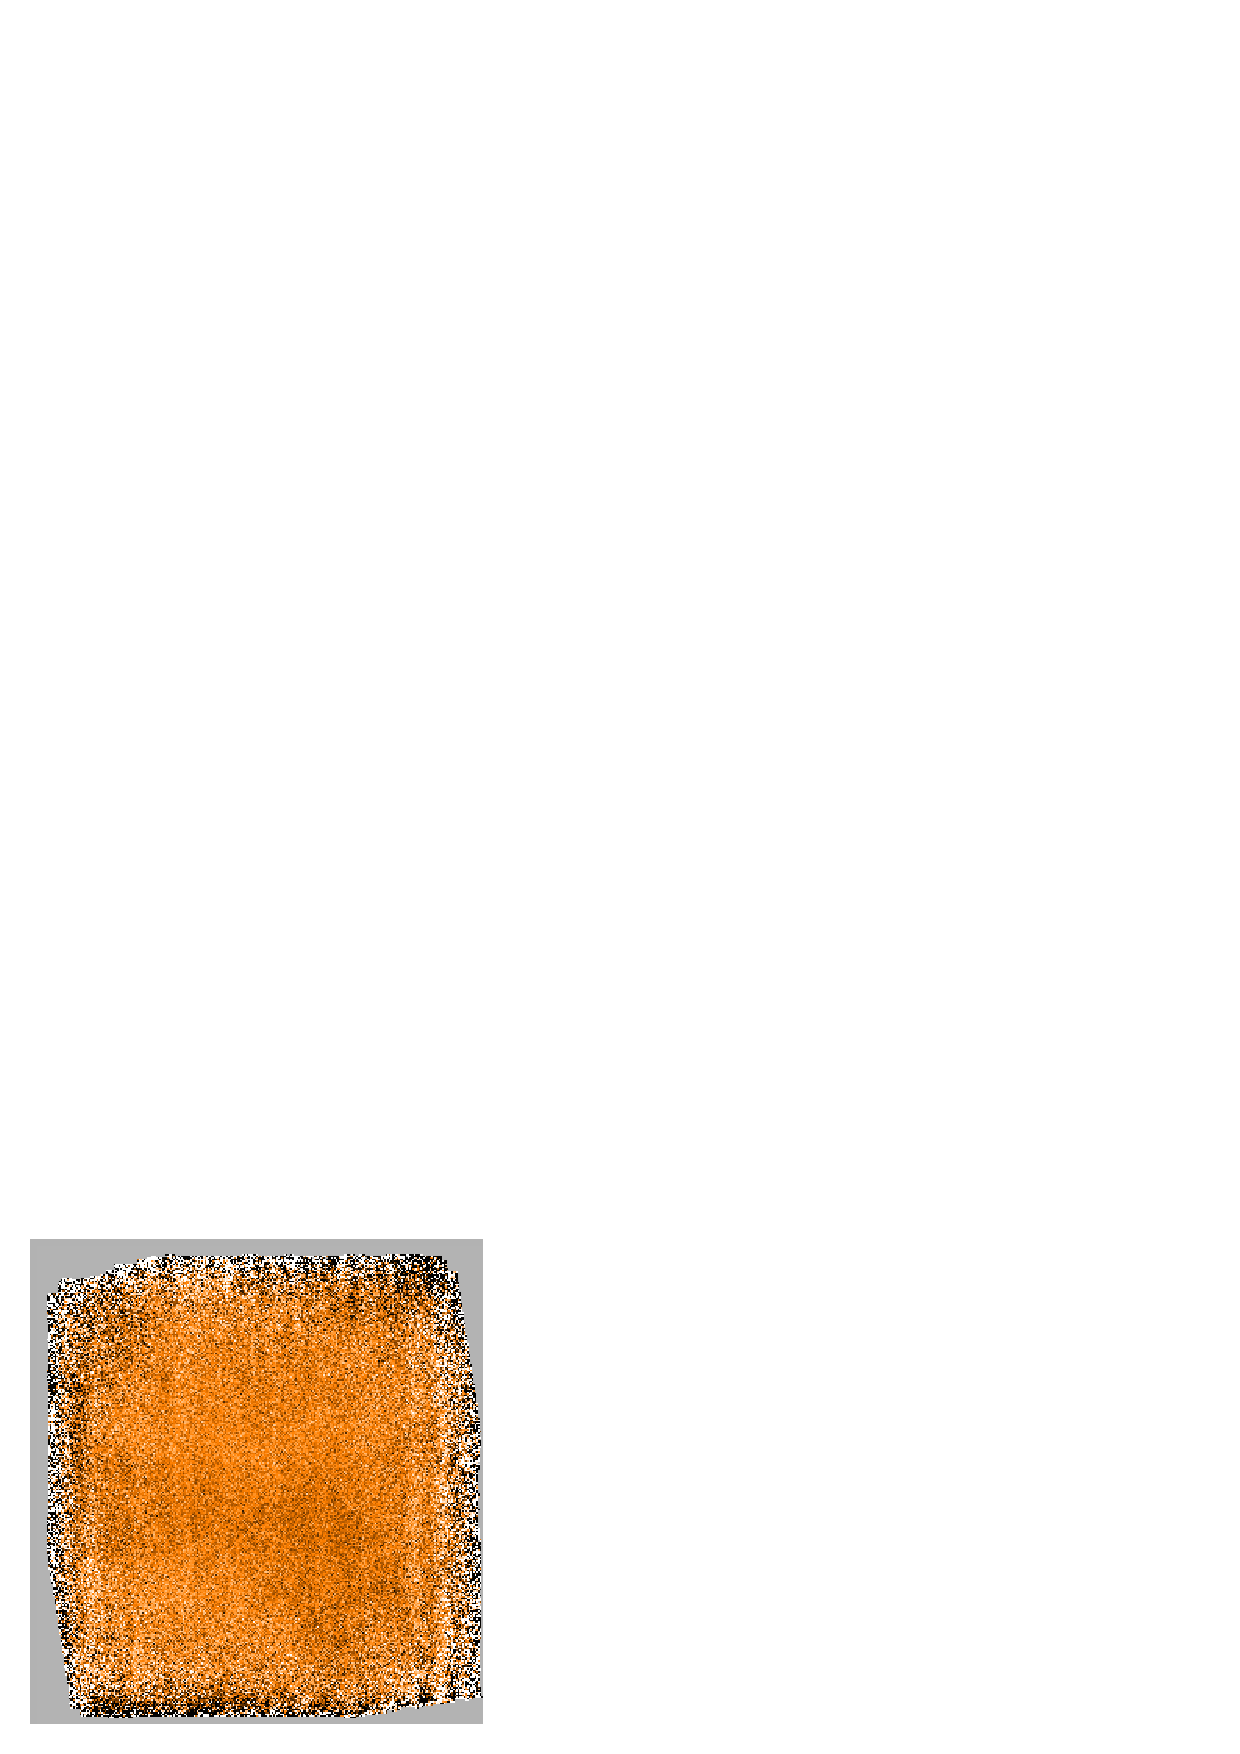
\includegraphics[width=0.49\linewidth]{sc19_cosmo_map}
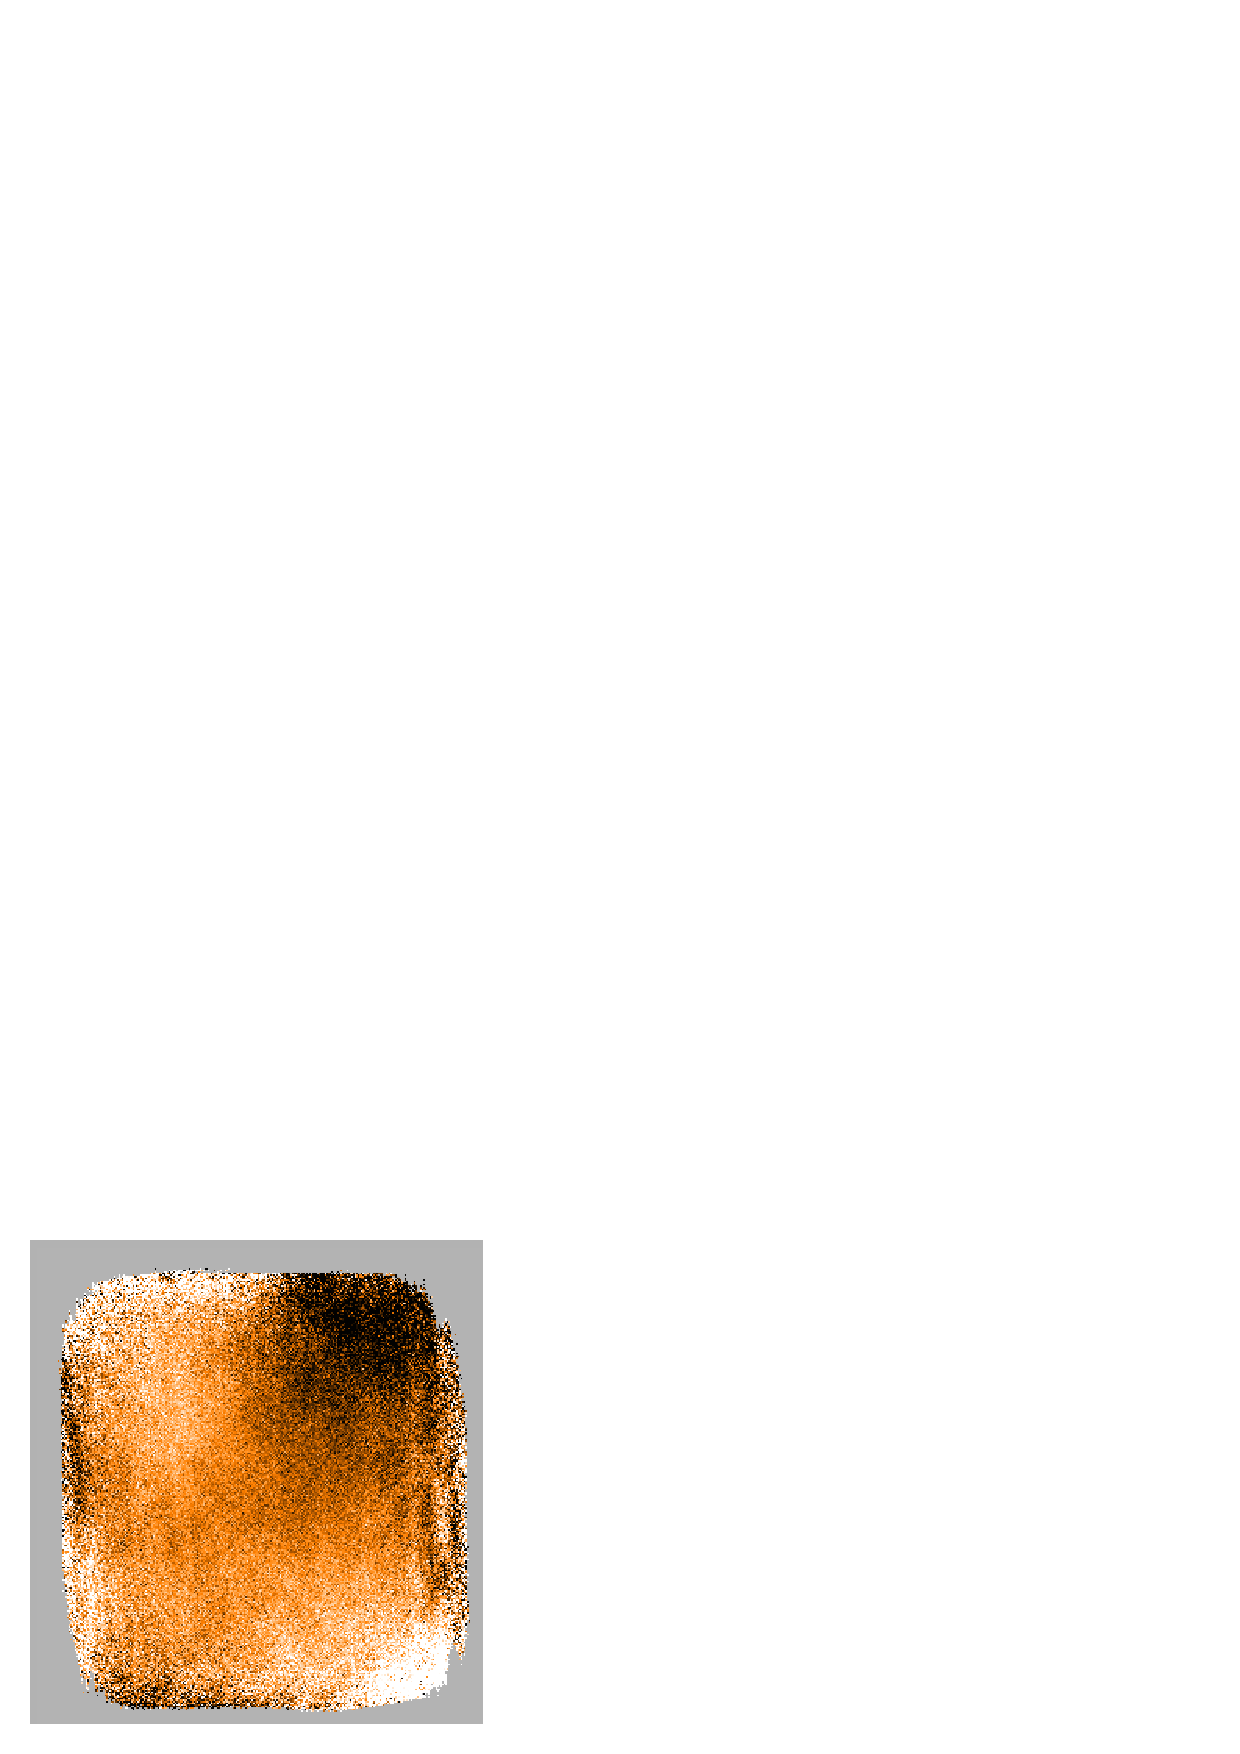
\includegraphics[width=0.49\linewidth]{sc19_cosmo_map_default} \\
\caption{Maps of a deep cosmology field towards the cluster MS0451, at
  450\micron. \textbf{Left:} map using the specialized
  \texttt{dimmconfig\_blank\_field.lis} which gives a significantly
  flatter result than \textbf{Right:} map using the default
  \texttt{dimmconfig.lis}.}
\label{fig:cosmomap}
\end{center}
\end{figure}

In order to optimally find sources that are the size of the telescope
beam, and suppress this residual large-scale noise, we provide a
\picard\ recipe (see Section~\ref{sec:fcf}) called
\\ \drrecipe{SCUBA2\_MATCHED\_FILTER}.

If there were no large-scale noise in the map, the filtered signal map
would be calculated as follows:
%
\begin{equation}
\mathcal{M} = \frac{[M(x,y)/\sigma^2(x,y)] \otimes P(x,y)}
  {[1/\sigma^2(x,y)] \otimes [P^2(x,y)]},
\end{equation}
%
where $M(x,y)$ and $\sigma(x,y)$ are the signal and RMS
noise maps produced by \smurf, and $P(x,y)$ is a map of the
PSF. Here `$\otimes$' denotes the 2-dimensional cross-correlation
operator. Similarly, the variance map would be calculated as
%
\begin{equation}
  \mathcal{N}^2 = \frac{1}{[1/\sigma^2(x,y)] \otimes [P^2(x,y)]}.
\end{equation}
%
This operation is equivalent to calculating the maximum-likelihood fit
of the PSF centered over every pixel in the map, taking into account
the noise. Presently $P$ is simply modeled as an ideal Gaussian
with a FWHM set to the diffraction limit of the telescope.

However, since there is large-scale (and therefore correlated from
pixel to pixel) noise, the recipe also has an additional step. It
first smooths the map by cross-correlating with a larger Gaussian
kernel to estimate the background, and then subtracts it from the
image. The same operation is also applied to the PSF to estimate the
effective shape of a point-source in this background-subtracted map.

Before applying the filter to our cosmology data, we first look at the
effect it has on the map of Uranus from Fig.~\ref{fig:itermap}. We
create a simple parameter file called \texttt{smooth.ini},
\begin{terminalv}
[SCUBA2_MATCHED_FILTER]
SMOOTH_FWHM = 15
\end{terminalv}
%
where \texttt{SMOOTH\_FWHM = 15} indicates that the background should
be estimated by first smoothing the map and PSF with a 15\,arcsec FWHM
Gaussian. Next, the recipe is executed as follows:
%
\begin{terminalv}
% picard -recpars smooth.ini SCUBA2_MATCHED_FILTER uranus.sdf
\end{terminalv}
%
The output of this operation is a smoothed image called
\texttt{uranus\_mf.sdf}. By default, the recipe automatically
normalizes the output such that the peak flux densities of point
sources are conserved. Note that the accuracy of this normalization
depends on how closely the real PSF matches the 7.5\,arcsec and
14\,arcsec full-width at half-maximum (FWHM) Gaussian shapes assumed
at 450\micron\ and 850\micron, respectively (an explicit PSF can
also be supplied using the \param{PSF\_MATCHFILTER} recipe
parameter).

\begin{figure}
\begin{center}
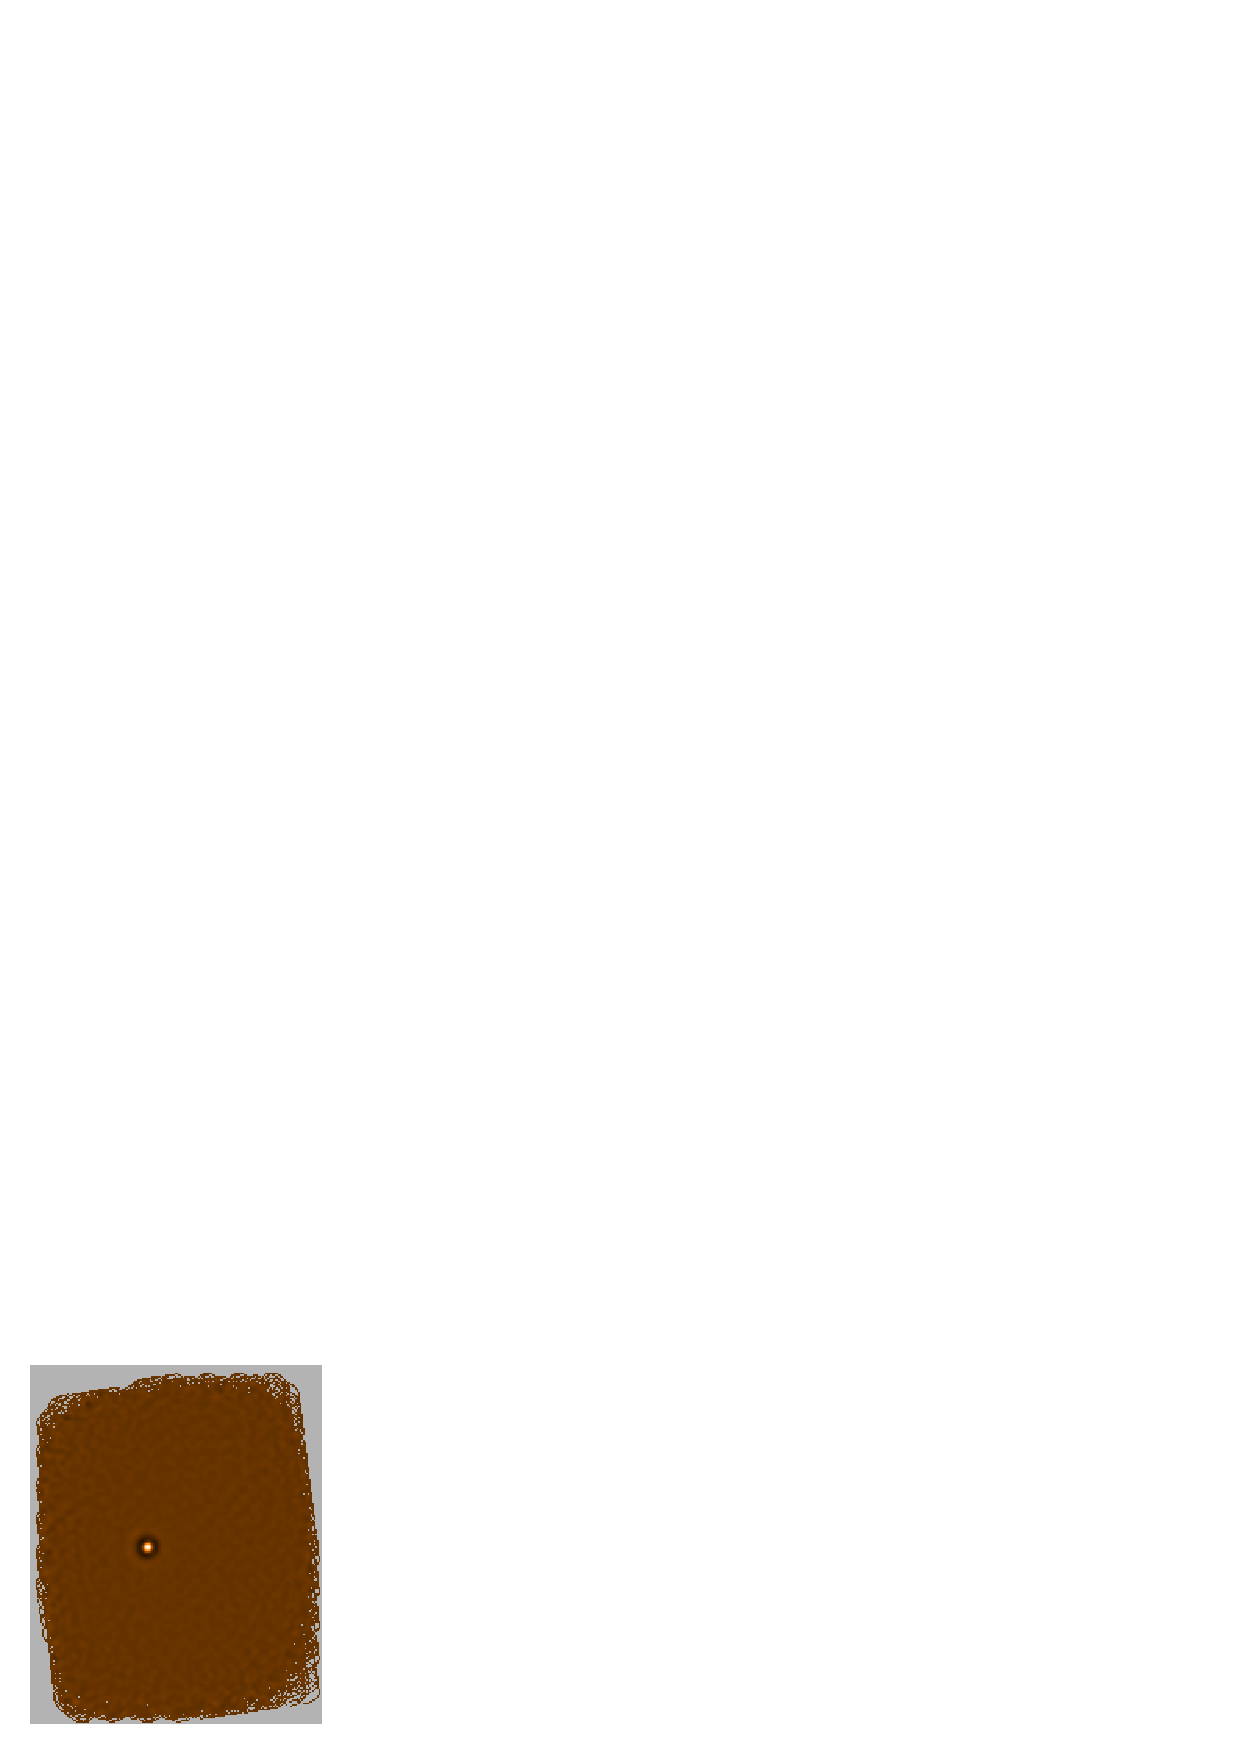
\includegraphics[width=0.46\linewidth]{sc19_uranus_filt}
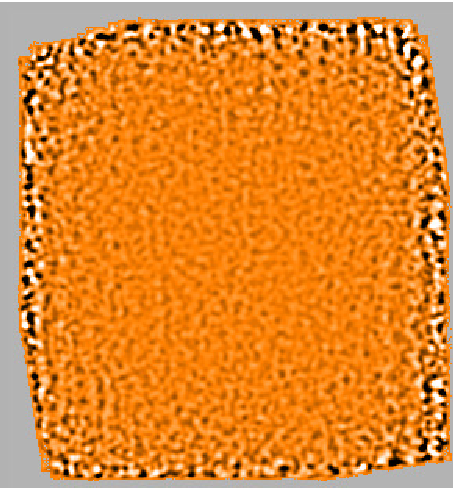
\includegraphics[width=0.525\linewidth]{sc19_cosmo_map_filt}
\caption{450\micron\ maps processed with the \picard\ recipe
  \texttt{SCUBA2\_MATCHED\_FILTER}, suppressing scales larger than
  15\,arcsec. \textbf{Left:} filtered map of Uranus from
  Fig.~\ref{fig:itermap}. \textbf{Right:} filtered version of deep
  cosmology map from left-hand panel of Fig.~\ref{fig:cosmomap}.}
\label{fig:cosmo_filt}
\end{center}
\end{figure}

The smoothed Uranus map is shown in Fig.~\ref{fig:cosmo_filt}. The map
is generally flatter than the raw output of \makemap, and the noise
level is significantly reduced. However, the price that we pay for
suppressing signal on scales larger than 15\,arcsec is visible as the
large negative ring around the source. For this particular case the
dip is about 10 per cent of the peak signal. In addition to ringing, the
filter attenuates the peak flux density of point sources. However, the
normalization applies a positive correction to preserve peak flux
densities, which results in an increased noise level.

Now that we know what this procedure does to a bright point source, we
proceed to filter the map of MS0451:

\begin{terminalv}
% picard -recpars smooth.ini SCUBA2_MATCHED_FILTER map450.sdf
\end{terminalv}

The smoothed map, \texttt{map450\_mf.sdf}, is shown next to Uranus in
Fig.~\ref{fig:cosmo_filt}. As hoped, this map has most of the
remaining large-scale residual structure removed, and in general the
noise is significantly reduced.

Finally, how should we find sources? The filtered map also contains a
VARIANCE component, so it is easy to produce a S/N map using the \Kappa\
task \makesnr:

\begin{terminalv}
% makesnr map450_mf map450_mf_snr
\end{terminalv}

The resulting map, \texttt{map450\_mf\_snr}, is shown in
Fig.~\ref{fig:cosmo_snr}. Compared to Fig.~\ref{fig:cosmo_filt} the
edges no longer appear as noisy because they have been down-weighted
by the larger noise values where there were less data.

\begin{figure}
\begin{center}
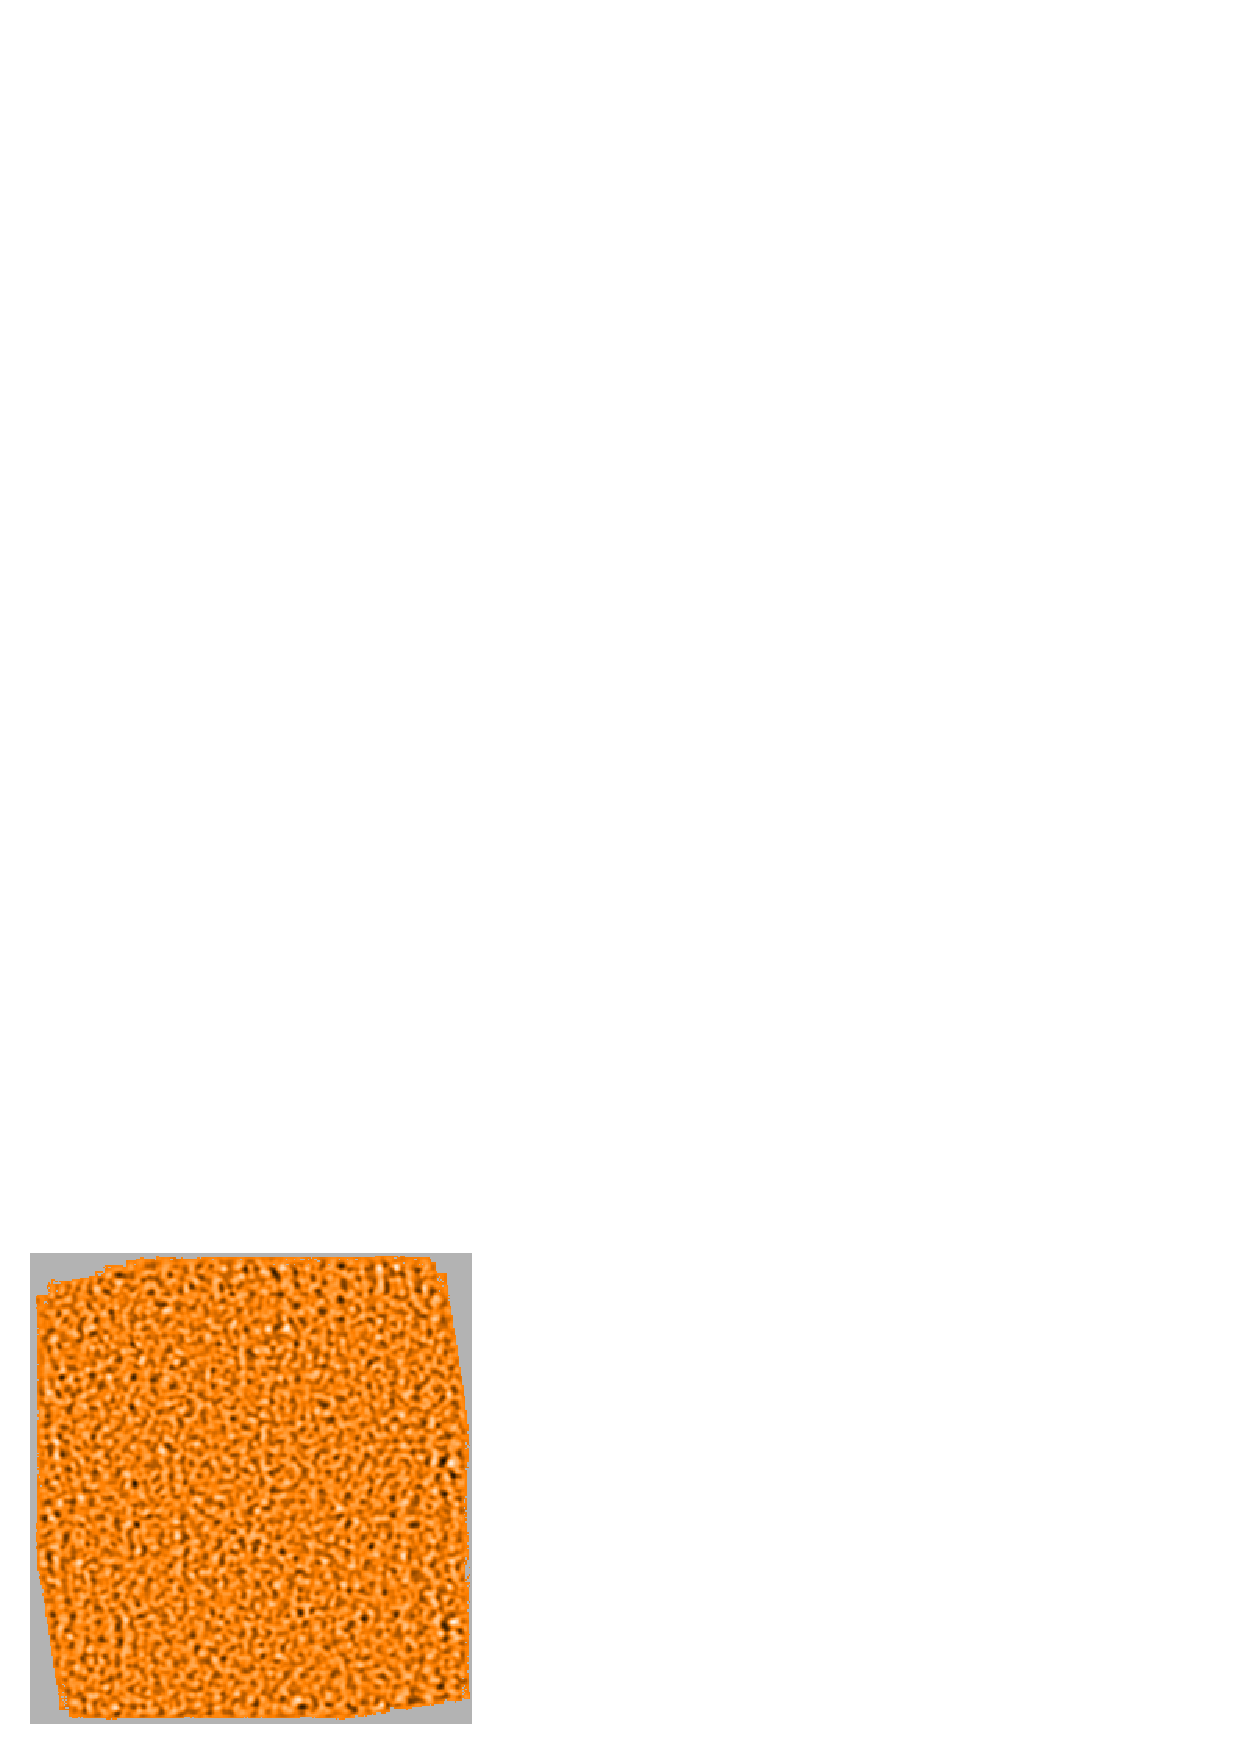
\includegraphics[width=0.49\linewidth]{sc19_cosmo_map_snr}
\caption{S/N map produced from the match-filtered image of the cluster
  MS0451 in Fig.~\ref{fig:cosmo_filt}, scaled from $-4\sigma$ (black)
  to $+4\sigma$ (white).}
\label{fig:cosmo_snr}
\end{center}
\end{figure}

A basic procedure for identifying sources would be to locate peaks
above some threshold S/N. However, as a word of caution, even after
all of these steps the noise may not be perfectly well-behaved. In
this example we do not expect any real astronomical source, so the S/N
map \emph{should\/} have a brightness distribution that resembles a
Gaussian with standard deviation $\sigma=1$ and mean zero. We perform
this comparison for the central $100 \times 100$ pixels of the S/N map
in Fig.~\ref{fig:cosmo_snrcompare}, well away from any edge
effects. In this case we find that the real distribution is slightly
narrower than expected, suggesting that the noise has been mildly
over-estimated.

\begin{figure}
\begin{center}
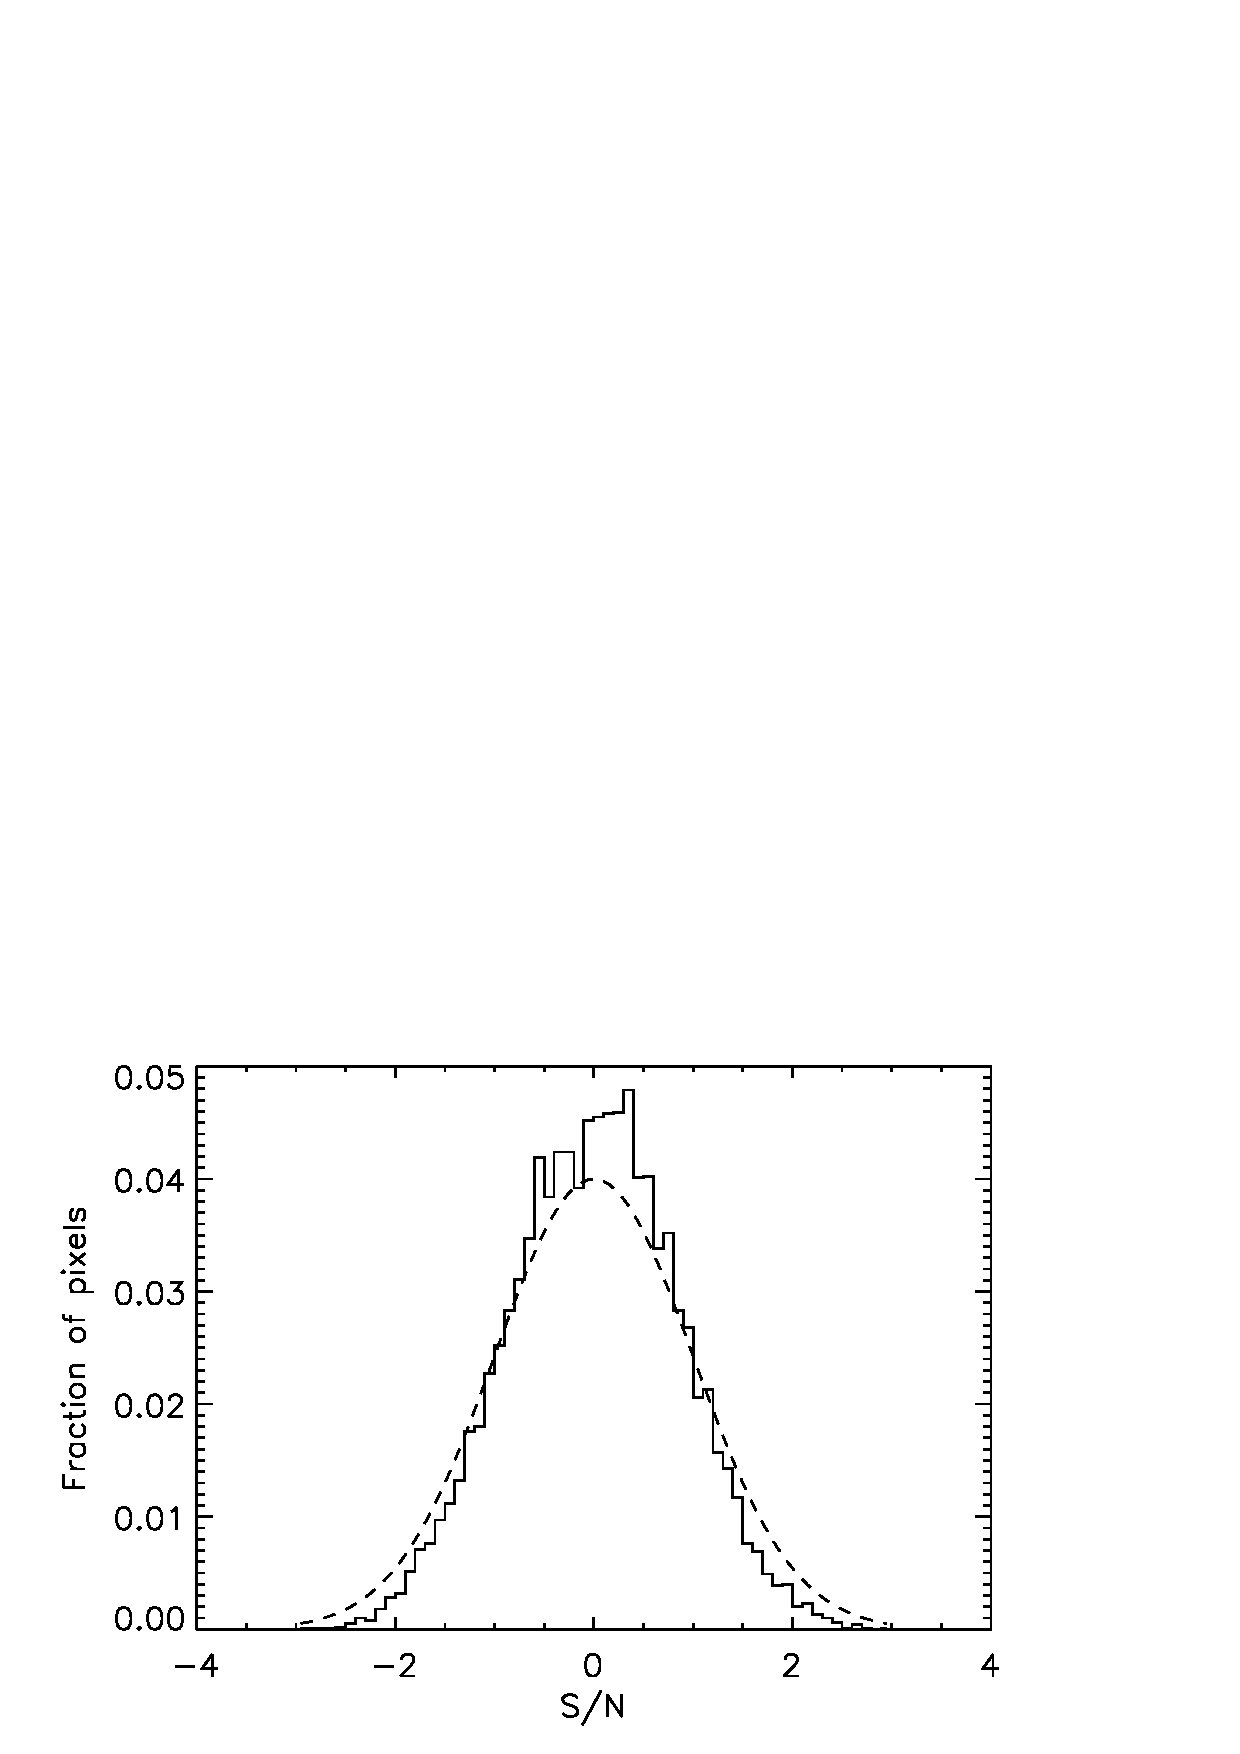
\includegraphics[width=0.8\linewidth]{sc19_cosmo_snrcompare}
\caption{The distribution of S/N for the central $100 \times 100$
  pixels of Fig.~\ref{fig:cosmo_filt} (histogram), compared with an
  ideal Gaussian distribution with mean zero and $\sigma=1$ (dashed
  line). The fact that the real distribution is narrower demonstrates
  that in this region of the map the noise is probably slightly
  over-estimated.}
\label{fig:cosmo_snrcompare}
\end{center}
\end{figure}

We recognize that noise characterization is of utmost importance to
the deep surveys, and we will continue to develop methods for
estimating the true noise distributions in the final maps (e.g., using
Monte Carlo simulations). Also, the Gaussian background noise
suppression currently implemented in the matched-filter is
isotropic. Clearly some of the residual large-scale noise has a
preferred direction (such as the vertical stripes in
Fig.~\ref{fig:cosmomap}). We are therefore investigating ways of
automatically estimating more efficient filters for specific map
geometries that will hopefully result in flatter maps, with reduced
negative ringing around sources.

As a parting word on this subject, we mention some other tests that
PIs should consider undertaking:

\begin{itemize}

\item Experiment with the size of the background suppression filter,
  as the large-scale noise depends on the scan pattern and state of
  the instrument when the data were taken. In this example, 15\,arcsec
  was chosen in order to remove the bulk of the stripes parallel to
  the edges of the map. A smaller filter will cause more ringing, and
  more attenuation of the peak value (as mentioned above this is
  corrected for in terms of absolute calibration, but the S/N is
  reduced). On the other hand, a larger filter will leave more of the
  large-scale noise features.

\item Split your data into mutually-exclusive subsets and produce
  independent maps. Are the highest S/N peaks detected in each of
  them?

\item Use \emph{jackknife} tests to verify the estimated noise levels,
  i.e.~produce two maps from independent portions of the data and
  difference them (e.g., using the \Kappa\ task \sub). This will
  remove any astronomical signal, but increase the noise by a factor
  of about $\sqrt{2}$. Is the standard deviation in the central pixels
  (where the noise should hopefully be uniform) roughly $\sqrt{2}$
  larger than the noise estimated for either of the original maps?

\item How many \emph{negative} peaks above a given S/N are there
  compared to the \emph{positive} peaks?

\end{itemize}

\subsection{\xlabel{Galactic}Extended Galactic Sources}
\label{sec:galactic}
In this section we shall focus on the reduction of extended, Galactic
sources. In the following example we produce a map of the Orion nebula
from two observations (\#22 \& \#23) taken on 16th February 2010. Two
alternative methods will be used. The first is more cumbersome, but
illustrates the use of \picard\ facilities for background removal,
cropping, and mosaicking. The second method uses an alternative DIMM
configuration aimed at maps of bright extended structures, and a
single call to \makemap.

\subsubsection{\xlabel{galacticpicard}Standard DIMM configuration + \picard}

If, as in this case, you have multiple observations contributing to
your map, each observation can be reduced separately, and then
combined to make the final map. Currently there is no advantage in
terms of data quality to reducing all observations simultaneously or
separately. However, the latter does allow the option of assessing the
individual maps before coadding and is the method followed in this
example.

When running the DIMM we select the default configuration file
\texttt{dimmconfig.lis}; the individual parameters of which are
described in Section~\ref{sec:maps}.

\begin{terminalv}
% makemap '$STARLINK_DIR/share/smurf/s8d20100216_00022_000?.sdf' Orion22 \
method=iterate config=^$STARLINK_DIR/share/smurf/dimmconfig.lis

% makemap '$STARLINK_DIR/share/smurf/s8d20100216_00023_000?.sdf' Orion23 \
method=iterate config=^$STARLINK_DIR/share/smurf/dimmconfig.lis
\end{terminalv}

\begin{figure}
\begin{center}
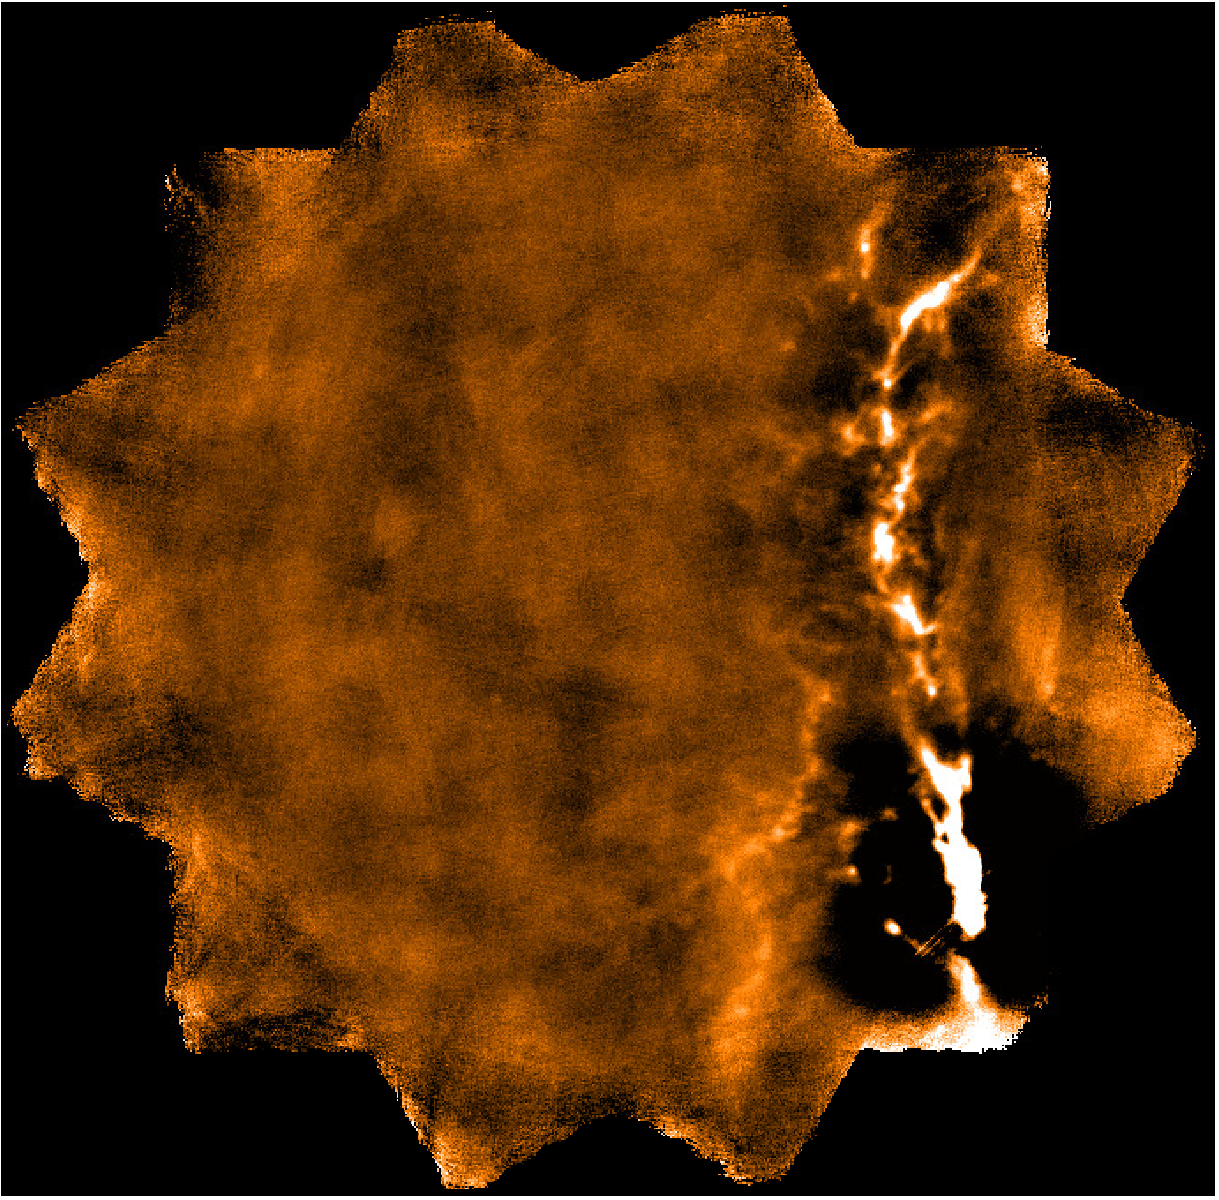
\includegraphics[width=0.49\hsize]{sc19_map22}
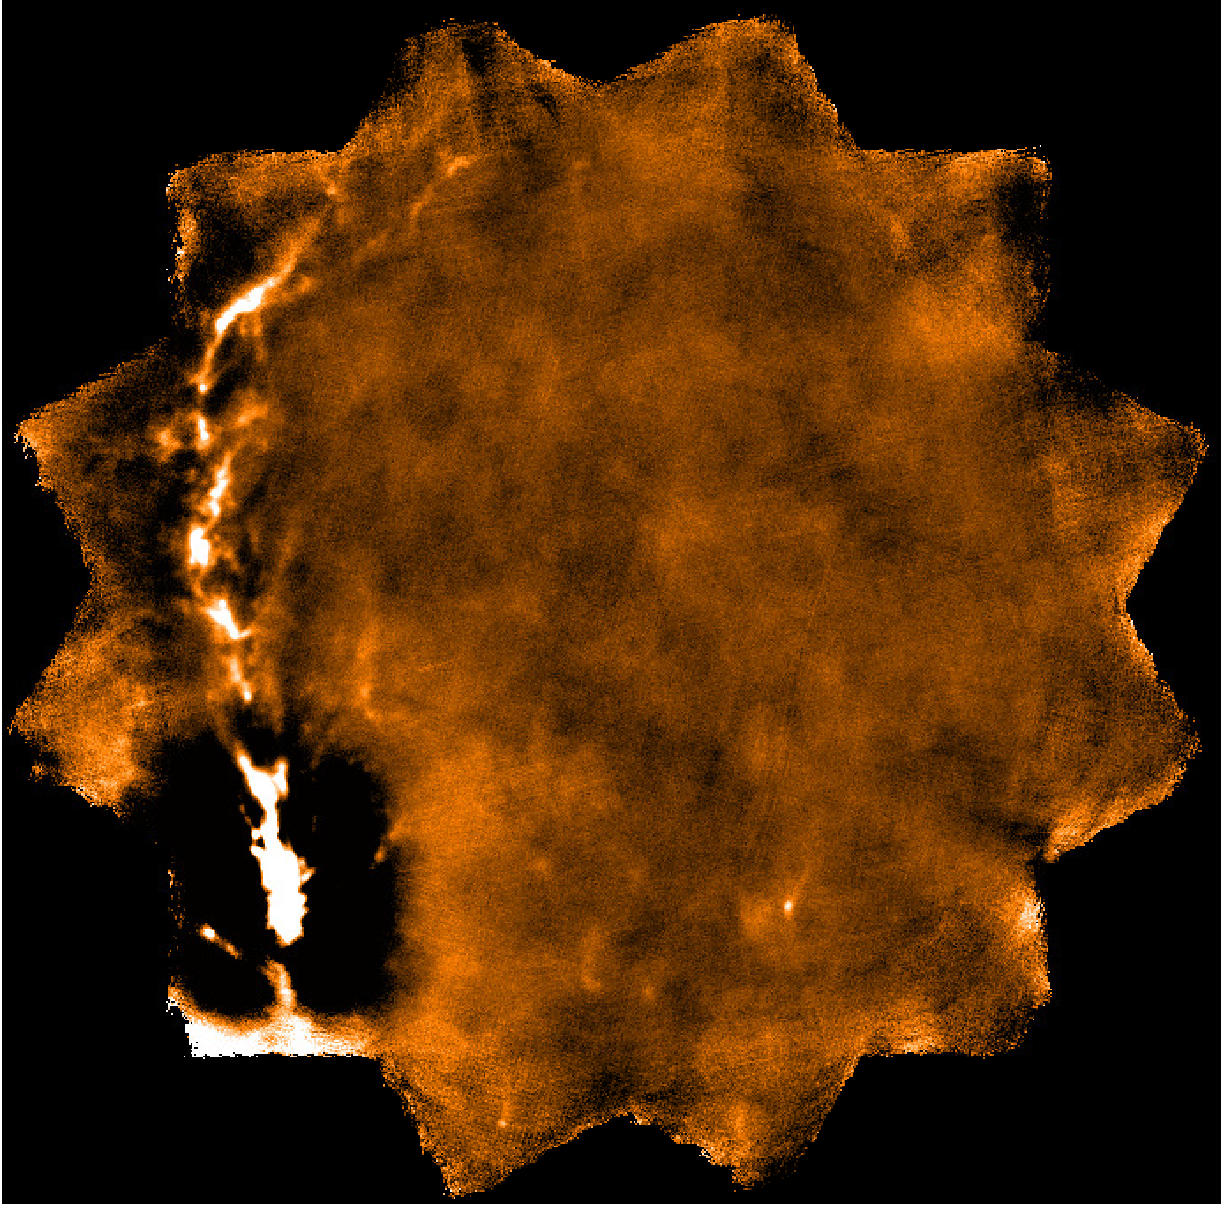
\includegraphics[width=0.49\hsize]{sc19_map23}
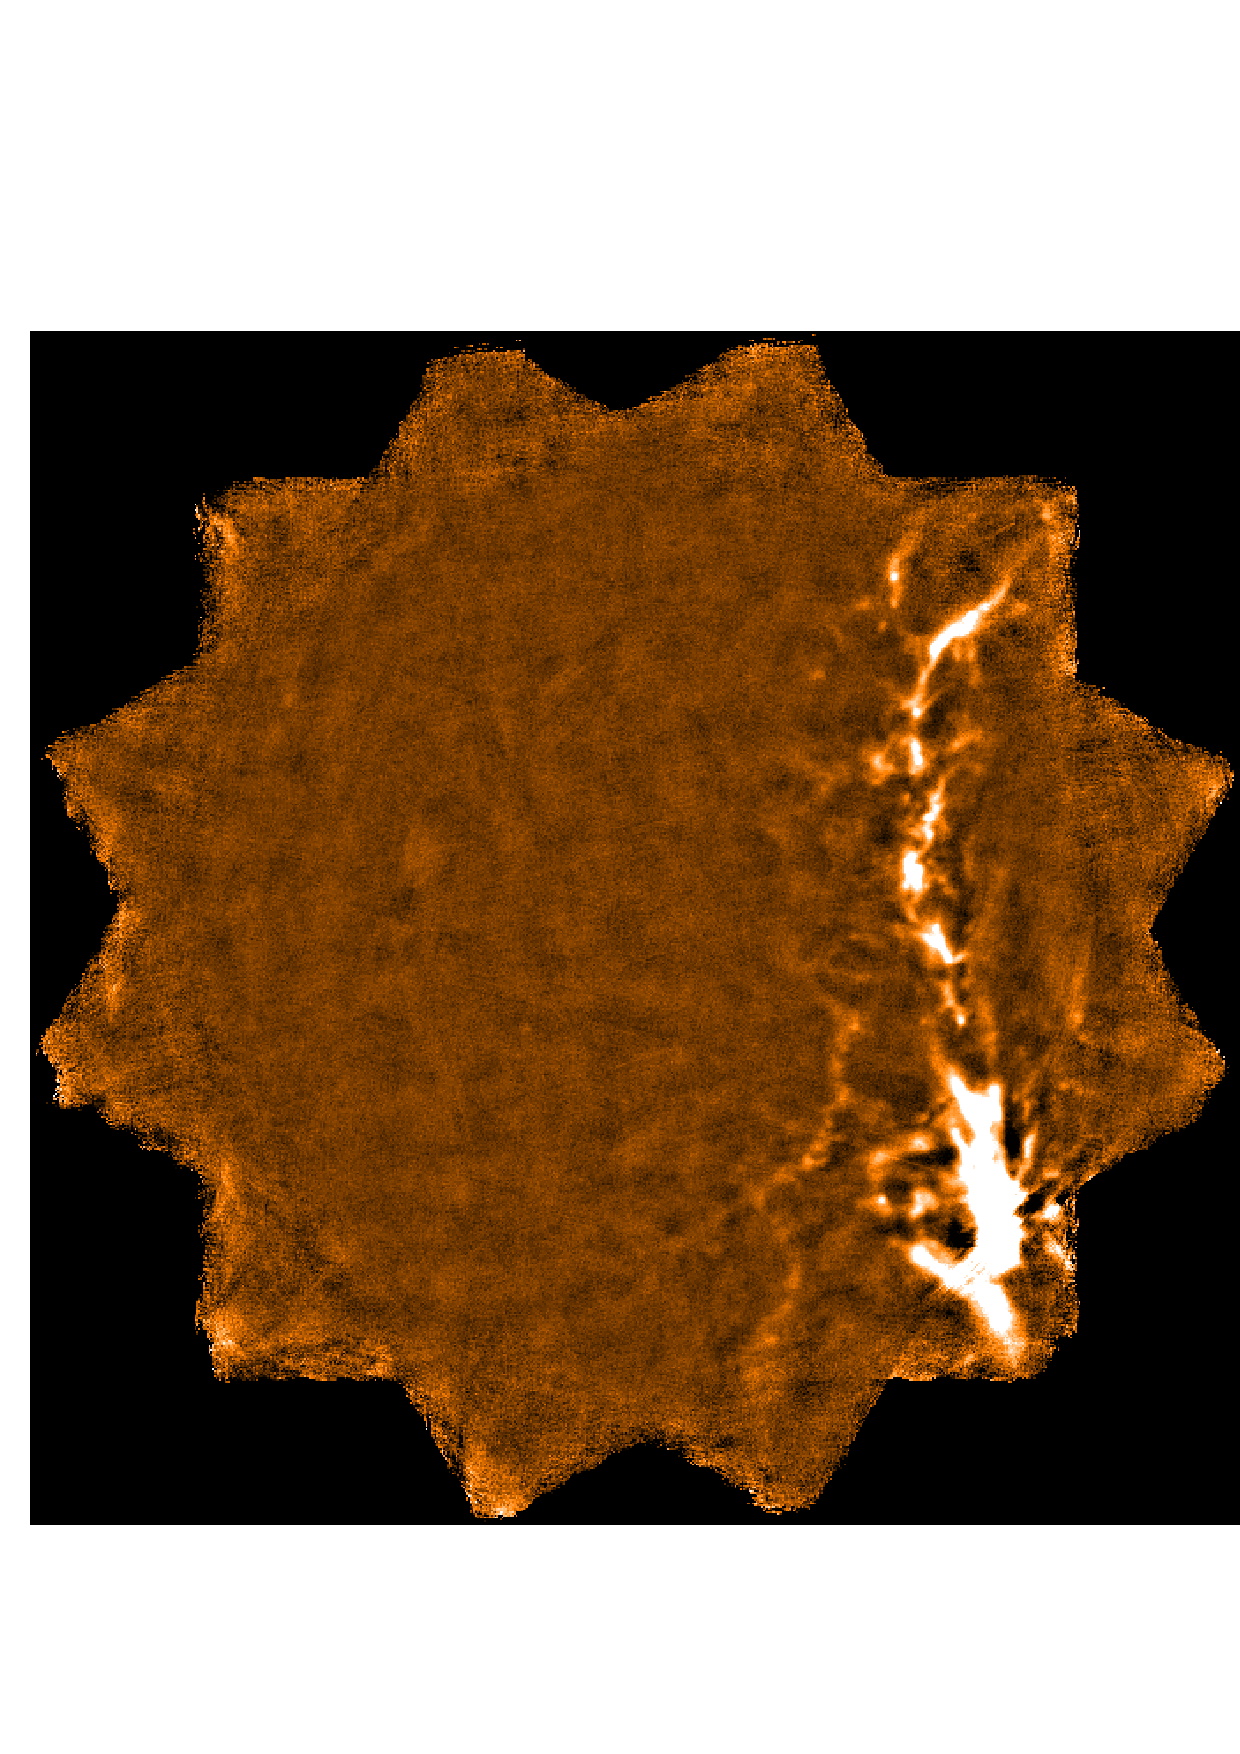
\includegraphics[width=0.49\hsize]{sc19_map22_back}
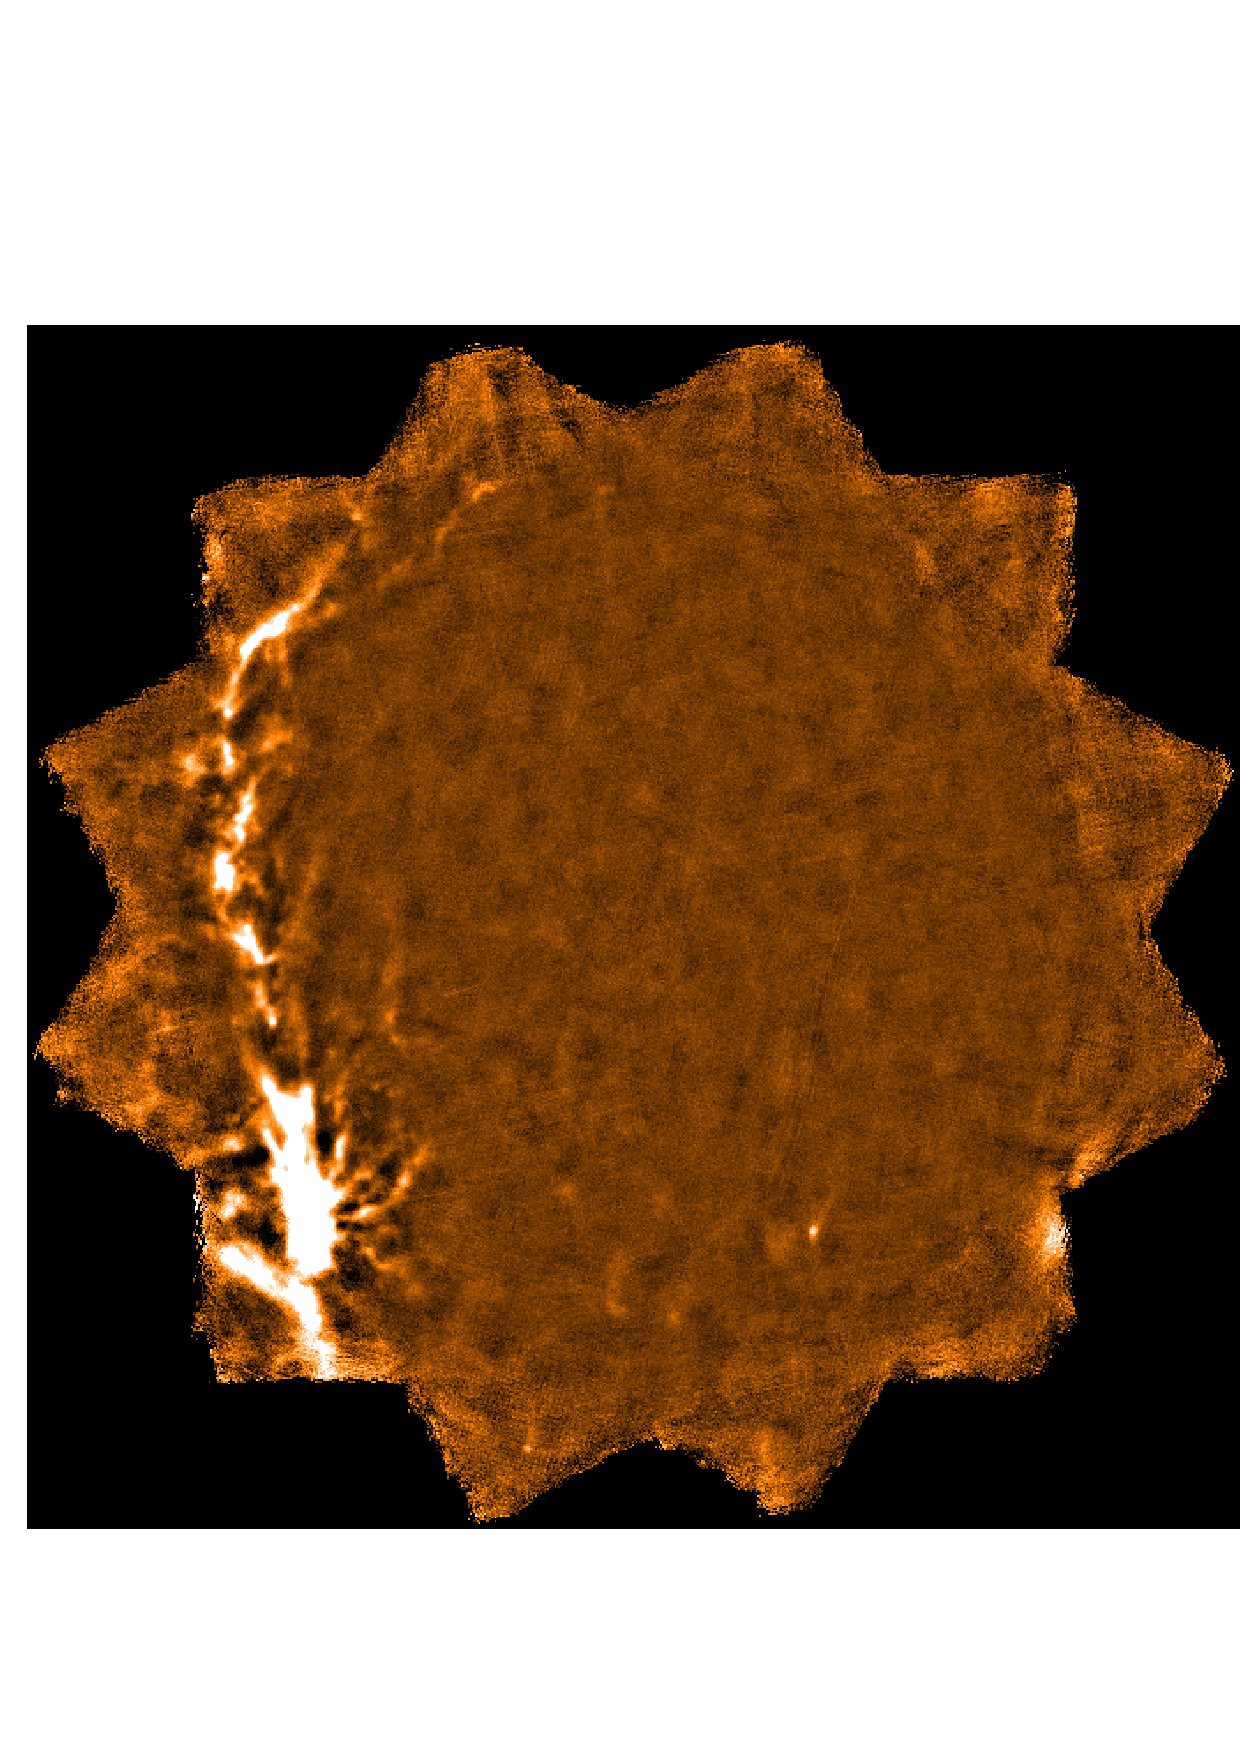
\includegraphics[width=0.49\hsize]{sc19_map23_back}
\caption{\textbf{Top row:} Orion22.sdf (left) and Orion23.sdf (right) maps from
  the mapmaker with no post processing. A patchy background and
  negative bowling around the strong sources is apparent. \textbf{Bottom row:}
  Orion22\_back.sdf (left) and Orion23\_back.sdf (right). The top row
  maps following processing with the \picard\ recipe \drrecipe{REMOVE\_BACKGROUND}
  using \findback\ with a box size of 30 pixels (120\,arcsec).}
\label{fig:orionmakemap}
\end{center}
\end{figure}

The map from each observation is shown on the top row of
Fig.~\ref{fig:orionmakemap}. Note that these maps were observed as a
series of rotating pong patterns to avoid repetition of any scan
direction, hence their distinctive shape.

The default configuration file is designed to preserve maximum flux,
however the difficulty of distinguishing between low frequency noise
and real extended source emission inevitably means that some low
frequency noise ends up in the final map. The maps show that although
extended emission has been recovered the background is far from flat,
displaying large scale patchiness as well as deep negative bowling
surrounding the strongest sources.

Both of these effects can be mitigated by post-processing
using the \picard\ recipe \drrecipe{REMOVE\_BACKGROUND}. A number of
different techniques are available in this recipe to control how the
background is removed.  In this example we have selected \cupid\
\findback\ which uses spatial filtering to remove structure on a size
scale less than that specififed by the
parameter \param{FINDBACK\_BOX}.  The modified parameter file
(\texttt{params.ini}) is shown below where the method is set to
\findback\ and the \findback\ box size to 30 pixels or 120\,arcsec
when using 4\,arcsec pixels:

\begin{terminalv}
[REMOVE_BACKGROUND]
BACKGROUND_FITMETHOD = findback
FINDBACK_BOX = 30
\end{terminalv}

Caution is advised when selecting the box size, with a smaller box
giving a flatter background but at the expense of source flux. This is
of particular importance to extended sources where the recovery of
faint emission is paramount.

\begin{terminalv}
% picard -recpars params.ini REMOVE_BACKGROUND Orion22.sdf
% picard -recpars params.ini REMOVE_BACKGROUND Orion23.sdf
\end{terminalv}

The background subtracted maps are shown on the bottom row of
Fig.~\ref{fig:orionmakemap} where both the bowling and uneven
background have been significantly improved. Before we combine the
maps we will first crop them to their originally requested size using
the \picard\ recipe \drrecipe{CROP\_JCMT\_IMAGES}.
\begin{terminalv}
% picard CROP_JCMT_IMAGES Orion22_back.sdf
% picard CROP_JCMT_IMAGES Orion23_back.sdf
\end{terminalv}

These cropped maps are then coadded using \drrecipe{MOSAIC\_JCMT\_IMAGES}. This
example utilises the default parameters where \wcsmosaic\ with variance
weighting is used for the mosaicking method although it can be
configured to use \makemos\ or to use a different \wcsmosaic\ method.
\begin{terminalv}
% picard MOSAIC_JCMT_IMAGES Orion2*_back_crop.sdf
\end{terminalv}

The key advantage to using the \picard\ recipe over standalone
\Kappa\ commands is that the exposure time image is also propagated
correctly to the output mosaic (it is stored in the
\texttt{.MORE.SMURF.EXP\_TIME} extension).

The final, coadded map is shown in Fig.~\ref{fig:orionmosaic}.

Note the output filename convention for each \picard\ recipe:
\drrecipe{REMOVE\_BACKGROUND} creates output files with the suffix
\texttt{\_back}, \drrecipe{CROP\_JCMT\_IMAGES} creates files with the
suffix \texttt{\_crop}, while \drrecipe{MOSAIC\_JCMT\_IMAGES} creates
files with the suffix \texttt{\_mos} appended to the \textit{last} input
filename.

\begin{figure}
\begin{center}
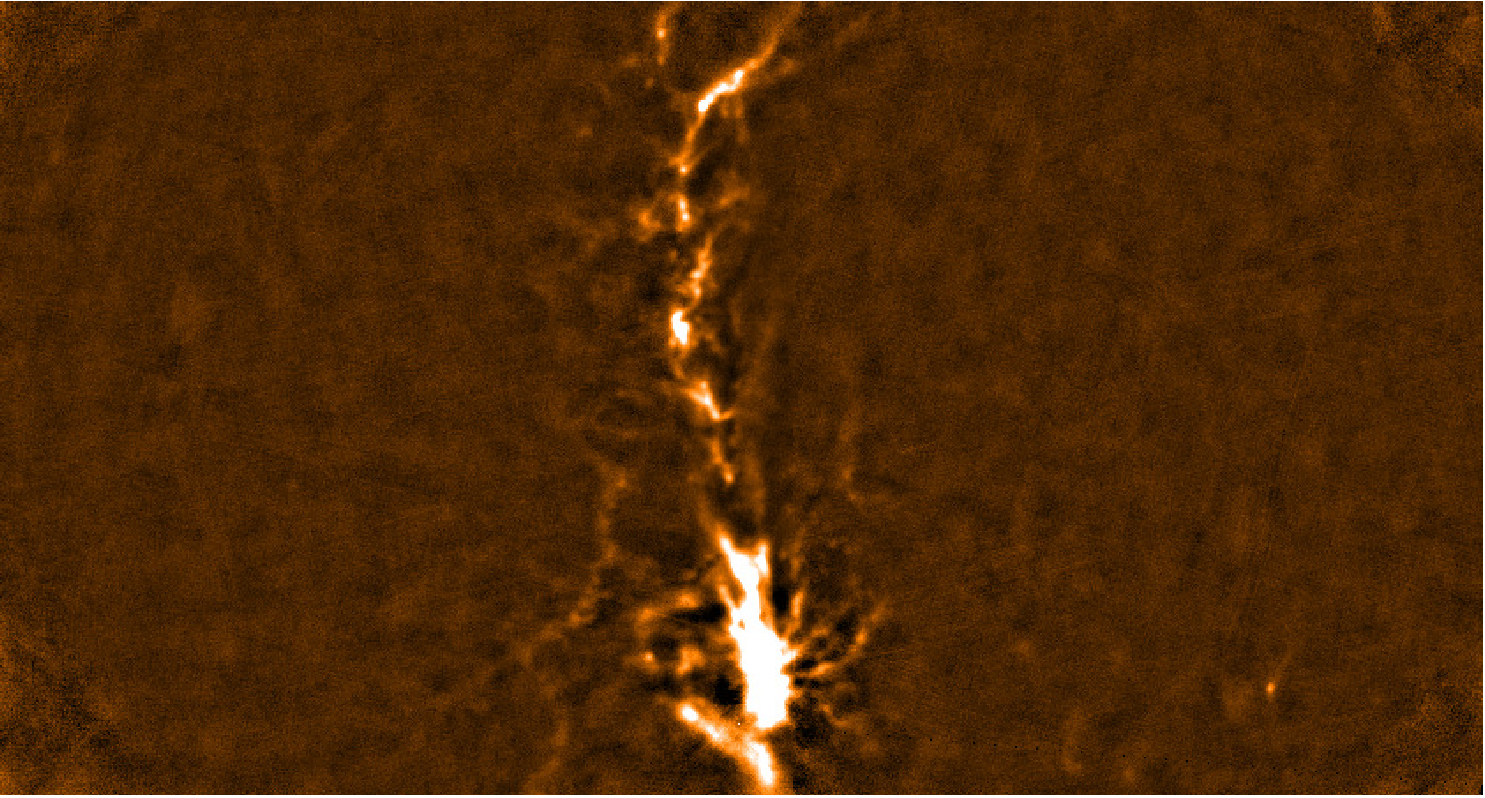
\includegraphics[width=\linewidth]{sc19_map22+23_back_crop_wcsmos}
\caption{Orion23\_back\_crop\_mos.sdf. The final map following the
  post processing steps of background removal, cropping and coadding
  with wcsmosaic.}
\label{fig:orionmosaic}
\end{center}
\end{figure}

\subsubsection{\xlabel{galacticextended}Bright / extended DIMM configuration}

The simpler method is to make a map from all of the data at once using
\texttt{dimmconfig\_bright\_extended.lis}:

\begin{terminalv}
% makemap "$STARLINK_DIR/share/smurf/s8d20100216_00022_0002[23].sdf" Orion \
method=iterate config=^$STARLINK_DIR/share/smurf/dimmconfig_bright_extended.lis
\end{terminalv}

The large-scale noise and negative bowling is compensated for using a
S/N-based zero mask during map-making. Everywhere the signal is below
this threshold (5-$\sigma$ by default), the map is set to zero for all
but the final iteration. The resulting map, and the location of the
iteratively-determined zero mask are shown in Fig.~\ref{fig:snrmask}.

\begin{figure}
\begin{center}
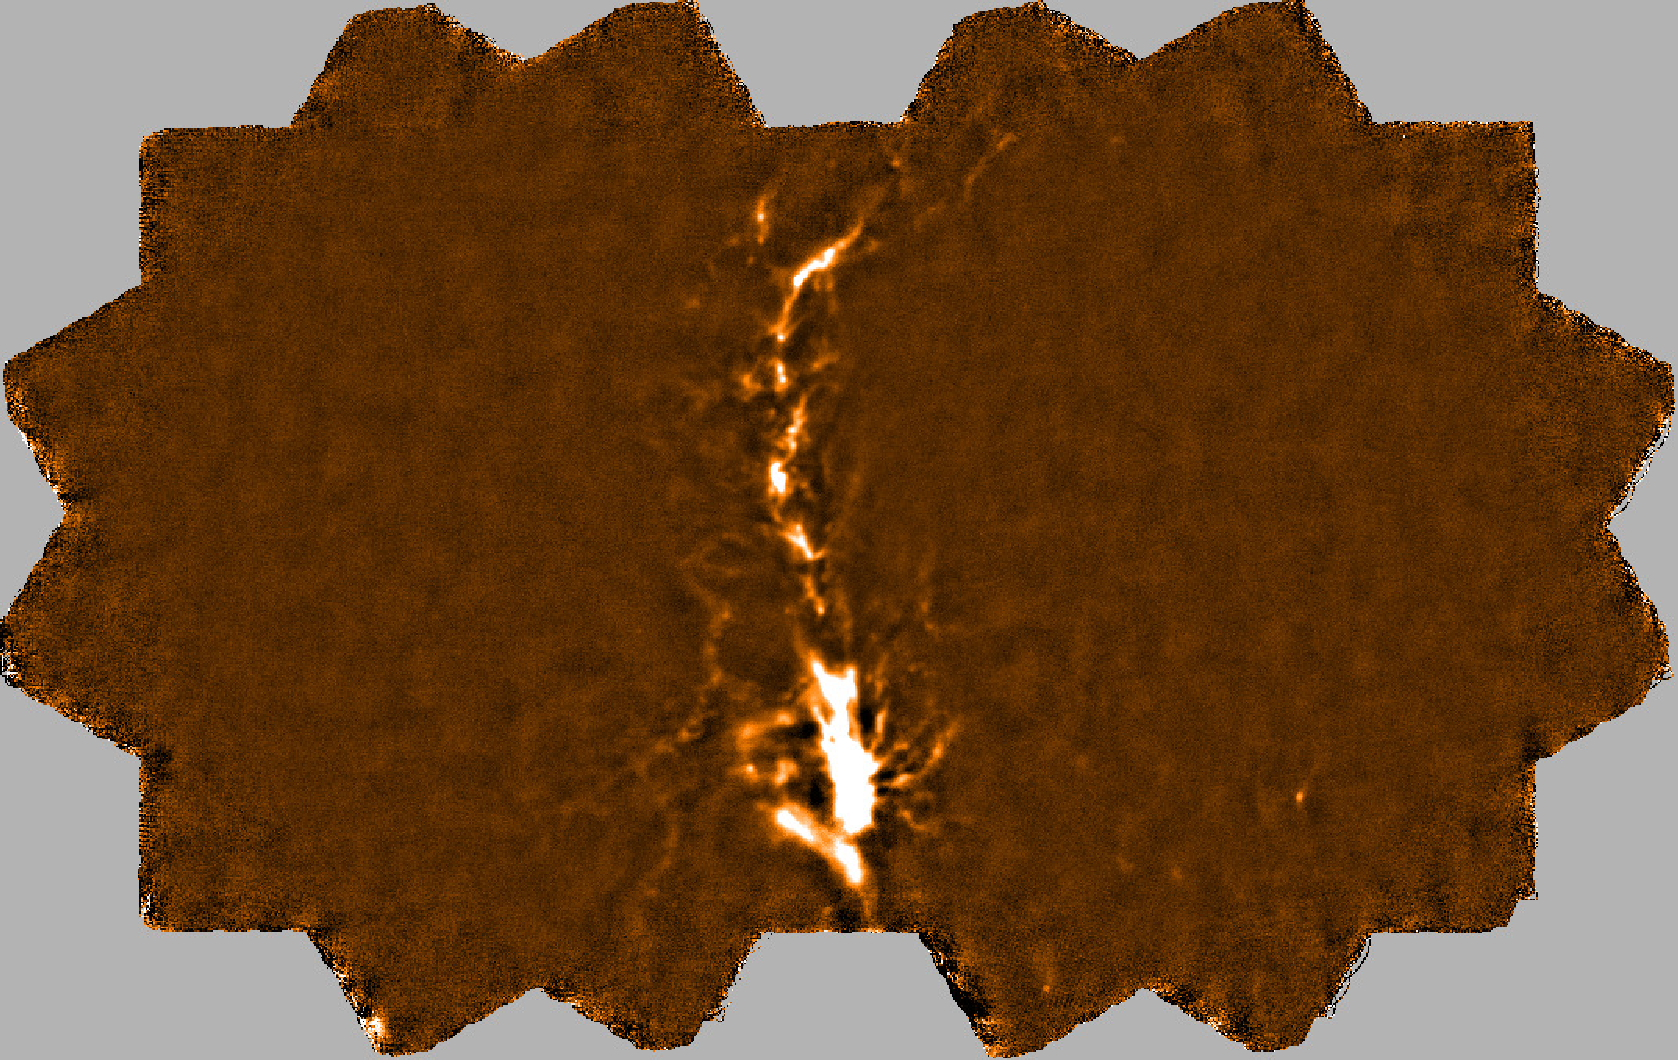
\includegraphics[width=\linewidth]{sc19_map22+23_brightextended}

\includegraphics[width=\linewidth]{sc19_map22+23_brightextended_mask}
\caption{\textbf{Top:} Map using all of the same data as in
  Fig.~\ref{fig:orionmakemap}, but processed simultaneously using a
  single call to \makemap\ with the specialized
  \texttt{dimmconfig\_bright\_extended.lis}. \textbf{Bottom:} The
  QUALITY component of the resulting map indicates (white) where the
  map has been constrained to zero after all but the final
  iteration. It is selected based on a S/N threshold.}
\label{fig:snrmask}
\end{center}
\end{figure}

\clearpage

\section{\xlabel{dataqual}Cheat sheet for checking data quality}
\label{sec:dataqual}

This section is a cheat sheet for a number of simple operations that
can be used to do quick checks of the data quality.

\subsection{\label{clean}Using \clean\ to help inspect time-series}

\clean\ can be used to do two basic tasks in one go: concatenate data
(with or without applying a flatfield); and cleaning (fix up steps and
spikes, remove the means, filter, remove common-mode etc.). It uses
the same configuration files as the iterative map-maker (though
ignoring the map-making specific items).

In this first basic example, we just want to clean up some data enough
to be able to see whether the bolometers have been flat-fielded
correctly, and more-or-less exhibit the same behaviour over time:

\begin{terminalv}
sc2clean $FILES clean config=^$STARLINK_DIR/share/smurf/dimmconfig.lis
\end{terminalv}

Here \texttt{\$FILES} can just be a single file from a subarray, or a
subset, e.g. \texttt{s8a20110417\_00051\_0003.sdf} (the first file
containing science data), \texttt{s8a20110417\_00051\_000"[1234]"}
(file 1 is a noise observation with shutter closed that gets ignored,
file 2 is a flatfield observation that will be used to override the
flatfield stored in the subsequent files 3 and 4 which are
concatenated together, the \texttt{.sdf} is optional),
\texttt{s8a20110417\_00051\_000\textbackslash?} (files 1 through 9),
\texttt{s8a20110417\_00051\_\textbackslash*} (the whole
observation). If you inspect the resulting \texttt{clean.sdf} in
\gaia\ (Section~\ref{sec:gaiacube}) and flip through the data cube you
should see all of the bolometers signals go up and down together with
about the same amplitude: the hope is that for a well-behaved
instrument you are mostly seeing sky noise variations that are seen
with roughly the same amplitude by all bolometers. Another common
feature, if the scans are particularly long and/or fast (e.g. 1\,deg
across), is strong periodic signals that are correlated with the scan
pattern. See Section~\ref{sec:state} -- in particular you will want to
plot \texttt{az} and \texttt{el} (the absolute azimuth and elevation),
and also \texttt{daz} and \texttt{del} (the azimuth and elevation
offsets from the map centre). This signal is usually
azimuth-correlated due to magnetic field pickup. It only shows up in
azimuth, because the instrument is on a Nasmyth platform and therefore
does not move in elevation.

Part of the reason the signals look the same is because they have been
flatfielded. You can turn off flatfielding using the \texttt{noflat}
option to \clean, and you should then see that all of the detector
amplitudes vary.

Another very useful option is to remove the common signal observed by
all of the bolometers. This may be accomplished by

\begin{terminalv}
sc2clean $FILES clean \
   config='"^$STARLINK_DIR/share/smurf/dimmconfig.lis,compreprocess=1"'
\end{terminalv}

The residual of this signal will exhibit second-order time-varying
correlated signals across the focal plane. Usually these are not very
large, but in some cases some very large localized signals have been
detected, particularly in the 850\,$\mu$m arrays in early 2011.

Another variation on this is to accentuate the residual low-frequency
noise by low-pass filtering the result. This can again be accomplished
by simply adding a filter command in the \texttt{config} parameter,
which in this case low-pass filters with a cutoff at 10\,Hz:

\begin{small}
\begin{terminalv}
sc2clean $FILES clean \
   config='"^$STARLINK_DIR/share/smurf/dimmconfig.lis,compreprocess=1,filt_edgelow=10"'
\end{terminalv}
\end{small}

Finally, in some cases you might just want to fit and remove
polynomial baselines from the bolometers (by default only the mean is
removed). This example will remove a line, but you can increase the
value of \texttt{order} to remove higher-order polynomials

\begin{terminalv}
sc2clean $FILES clean \
   config='"^$STARLINK_DIR/share/smurf/dimmconfig.lis,order=1"'
\end{terminalv}

\subsection{\label{caldata}Looking at calibration data}

Currently all science observations are preceded by two calibrations:
a short shutter-closed integration (file 1), followed by a ``sky
flat'' to determine the response of all the bolometers to a current
ramp through their heater resistors with the shutter open (file 2).
The science observations are all subsequent files, except for the last
which is also a sky flat.

The shutter-closed integrations can be useful to track the array
sensitivity independent of sky conditions. You can run these files (or
the science data files as well) through \calcnoise\ (the NEP map for
the subarray will be stored in the \texttt{.MORE.SMURF.NEP} extension
of the output NDF \texttt{s8a\_noise.sdf}):

\begin{terminalv}
calcnoise s8a20110417_00051_0001 s8a_noise method=! power=!
\end{terminalv}

The sky flats can be used to calculate responsivity images using
\calcflat:

\begin{terminalv}
calcflat s8a20110417_00051_0002 s8a_flat method=! resp=s8a_resp respmask
\end{terminalv}

The resulting \texttt{s8a\_flat.sdf} contains a data cube of the data used
to fit the responsivity (stacking several heater ramps together -- it
is easy to see bizarre/non-linear detectors that will subsequently be
flagged and removed), and the actual responsivity image is stored in
\texttt{s8a\_resp.sdf}.

\begin{thebibliography}{}
\addcontentsline{toc}{section}{References}

\bibitem{smurf}
Chapin~E.~L., et~al., 2009, \textit{SMURF -- Sub-Millimetre User Reduction
Facility},
\xref{Starlink User Note 258}{sun258}{}

\bibitem{ssds}
Currie~M.~J., Wallace~P.~T., Warren-Smith~R.~F., 1989, \textit{Starlink Standard Data Structures}, \xref{Starlink General Paper 38.2}{sgp38}{}

\bibitem{kappa}
Currie~M.~J., 1997, \textit{KAPPA --- Kernel Application Package},
\xref{Starlink User Note 95}{sun95}{}

\bibitem{gaia}
Draper~P.~W., 1997, \textit{GAIA -- Graphical Astronomy and Image
Analysis Tool},
\xref{Starlink User Note 214}{sun214}{}

\bibitem{sc2ana005}
Scott~D., Van Engelen~A., 2005, \textit{Scan Mode Strategies for
  SCUBA-2}, SCUBA-2 Data Reduction document SC2/ANA/S210/005

\bibitem{dempsey-spie}
Dempsey~J.~T., Friberg~P., Jenness~T., Bintley~D., Holland~W.~S., 2010
\textit{Extinction correction and on-sky calibration of SCUBA-2},
Proc.\ SPIE, 7741 (DOI:10.1117/12.856476)

\bibitem{archibald}
Archibald,~E.~N., et~al, 2002, \textit{On the atmospheric limitations of ground-based submillimetre astronomy using array receivers},
MNRAS, 336, 1-13

\bibitem{flux1}
Jenness~T., et~al, 2002, \textit{Towards the automated reduction and calibration of SCUBA data from the James Clerk Maxwell Telescope},
MNRAS, 336, 14-21

\bibitem{flux2}
Barnard,~V.~E., 2005,\textit{A summary of the search for new Submillimetre Secondary Calibrators},
Tech.\ Rep.\ SCD/SN/011, Joint Astronomy Centre

\end{thebibliography}

\newpage
\appendix

\section{\xlabel{Dataissues}Data Characteristics and Issues}
\label{sec:Issues}

S2SRO data, due to our changing understanding of the instrument during
shared risks observing, presents some particular challenges.

In order to illustrate in more detail some characteristics and issues
associated with the SCUBA-2 data taken for the S2SRO, we will walk
through an attempt to manually reduce a 850\micron\ observation on
CRL\,618 taken as observation 28 on 20100217.

\subsection{\xlabel{intro2}Introduction data issues}
\label{sec:intro2}

There is no recommended procedure for manually reducing SCUBA-2 data,
hence what follows is mainly intended to show the data issues rather
than deliver a science product. Typically manual processing will
remain inferior to the output of the iterative mapmaker. \textbf{Note:}
a number of measures will be taken to address some of the issues seen
during the S2SRO when upgrading SCUBA-2 to its full complement of 8
arrays. In particular in connection to the 30-sec fridge cycle, which
dominates the common-mode signal, and a thermal gradient across the
array that prevented the use of bolometers around the edge.

A listing of the observation directory shows the following:

\begin{terminalv}
 6956 s8d20100223_00017_0001.sdf
34140 s8d20100223_00017_0002.sdf
34140 s8d20100223_00017_0003.sdf
34140 s8d20100223_00017_0004.sdf
34140 s8d20100223_00017_0005.sdf
34140 s8d20100223_00017_0006.sdf
 6956 s8d20100223_00017_0007.sdf
\end{terminalv}

As explained in the main section of the manual, the first and last
files typically are `dark' or `flatfield ramp' observations. The
remaining files can all be concatenated without resulting in too large
a data set (which for science observations often will not be true
unfortunately).

\begin{terminalv}
% cp (raw data dir)/*.sdf .
% sc2concat in=s8d\*.sdf out=sc17_con
\end{terminalv}

\subsection{\xlabel{Tracking}Telescope tracking}
\label{sec:tracking}

A first inspection can be made of the tracking of the telescope by
inspecting the JCMT state structure in the headers:

\begin{terminalv}
% jcmtstate2cat sc17_con > sc17_con.cat
% topcat -f tst sc17_con.cat
\end{terminalv}

Select a 2-D image panel and the columns \texttt{x = TCS\_TR\_AC1, y =
TCS\_TR\_AC2} to show the actual tracking on the sky.  Each point
marks the position of tracking center for each of the 200~Hz samples.
By contrast the demanded tracking can be plotted using
\texttt{x~=~TCS\_TR\_DC1, y~=~TCS\_TR\_DC2}. The resulting figures are
shown in Fig.~\ref{fig:tracking}.

\begin{figure}[ht]
\begin{center}
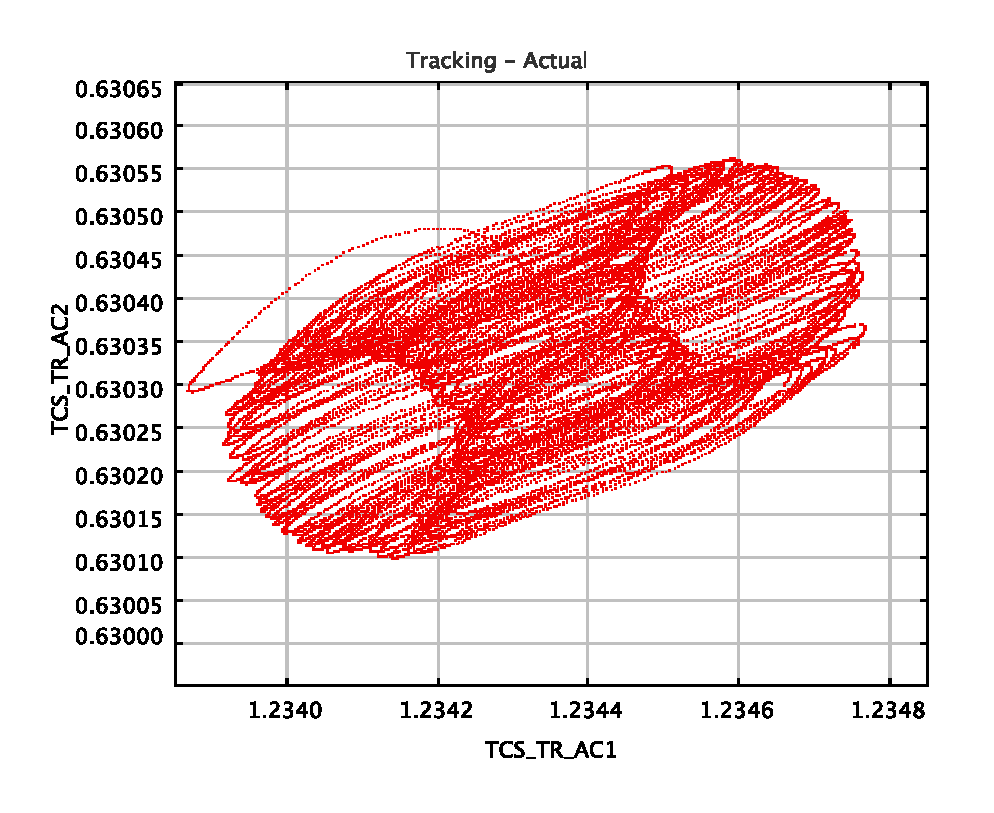
\includegraphics[width=0.45\linewidth]{sc19_tracking_actual}
\hspace{0.03\linewidth}
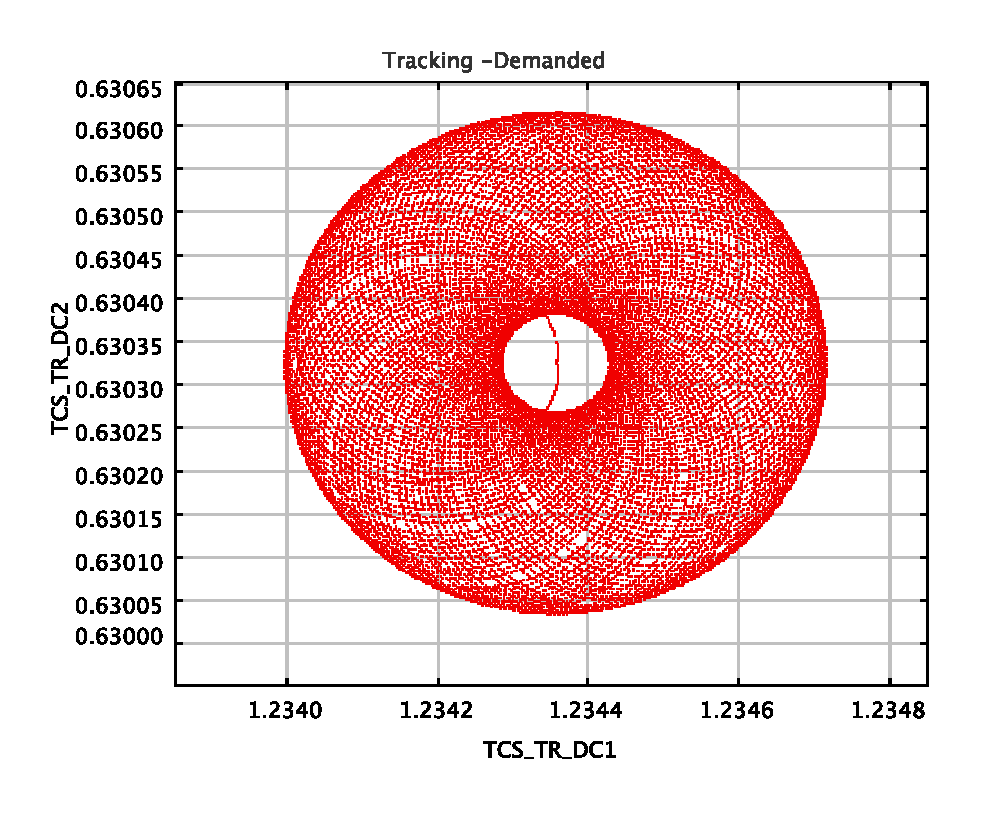
\includegraphics[width=0.45\linewidth]{sc19_tracking_demand}
\caption{\textsl{left:} Actual tracking; \textsl{Right:} Demanded tracking }
\label{fig:tracking}
\end{center}
\end{figure}

Obviously, for this observation the telescope failed to follow the
demanded daisy pattern due to its acceleration limits. This failure to
follow the demanded daisy pattern is often seen at higher elevations
(this observation was at an elevation of approximately 72\,deg). The
demanded daisy is 120\,arcsec across, i.e.\ even for the failed
pattern a 3\,arcmin field was almost always covered by the footprint
of the bolometer array.

Hence, although in general not disastrous for compact daisy fields,
the distribution of the tracking points may result in more systematics
across the field. In particular the diagonal pattern can result in a
`groove' in the final image when using the standard configuration file
in DIMM. Switching to \texttt{dimmconfig\_bright\_compact.lis}
can help.


\subsection{\xlabel{flatfield2}Flat field}
\label{sec:flatfield2}

\textsl{Note:} As explained in \S\ref{sec:sro:flatfields}, observations
taken after 20100223UT include a fast flatfield ramp at their start
and end. \smurf\ will use these to calculate the flatfield
dynamically. Earlier observations have a flatfield in their headers
calculated by the online system from an explicit flatfield observation
taken some time prior to the observation. These flatfields are less
reliable due to the variability of flatfields and the observations
should be treated with caution. It is recommended that \flatfield\ and
\copyflat\ should be used to re-calculate and re-insert the flatfield
using the, now default, better ramp-fitting techniques.

The above \concat\  command applies the flatfield to the data (it
does so by default). Collapsing the time series of the concatenated
and flatfielded file to calculate the mean signal for each bolometer
results in Fig.~\ref{fig:concollapse} showing the bolometer map for
the s8d array used during the S2SRO: a number of \textsl{dead} columns
can be seen as well as regions around the perimeter where the thermal
gradient caused problems biasing bolometers.

\begin{figure}[ht]
\begin{center}
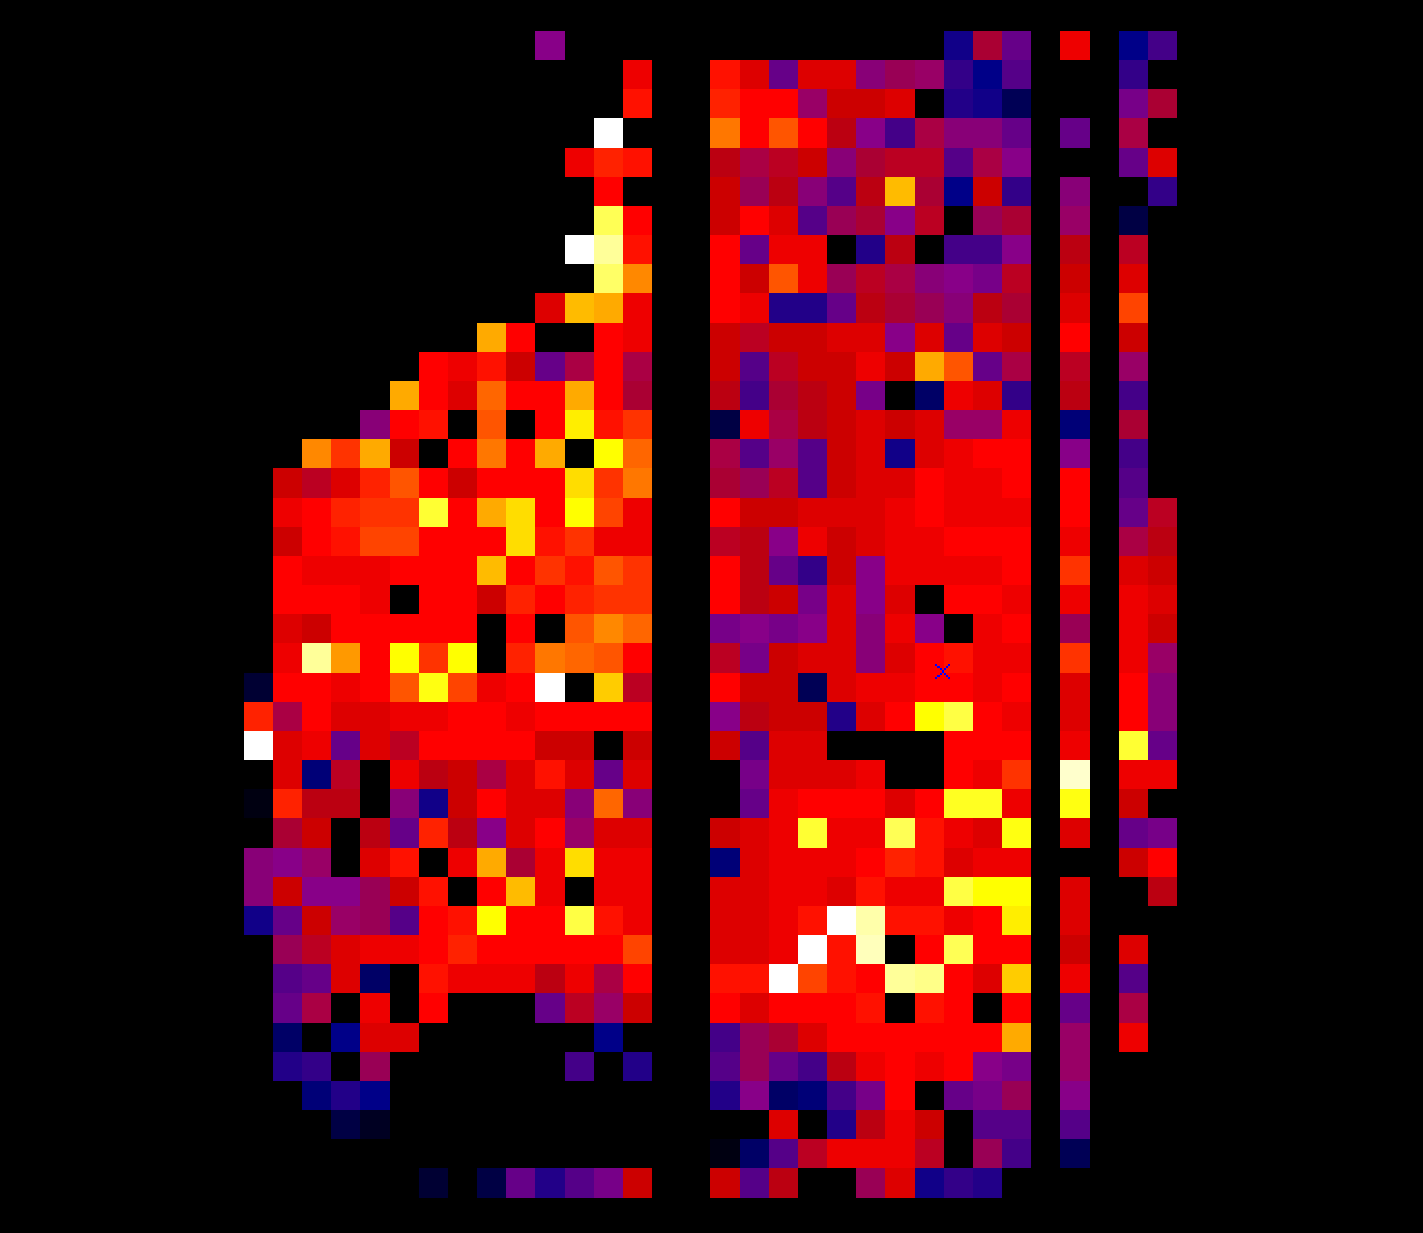
\includegraphics[width=0.45\linewidth]{sc19_con_collapse}
\caption{Mean signal in time-series }
\label{fig:concollapse}
\end{center}
\end{figure}

The range of the mean value in the map is very large: from $-$28 to
30. An inspection of the cube shows that much of this is caused by
differing DC levels across the bolometers. The DC term can be removed
using \clean\  (\mfittrend\ can be used as well). In general, for
relatively compact sources it should be safe to remove a first order
baseline to also account for a monotonic drift component in the time
series.

\begin{terminalv}
% cat my_sc2clean_bsl.def
order=1
dcfitbox = 0
spikethresh = 0

% sc2clean sc17_con sc17_conbsl config=^my_sc2clean_bsl.def
\end{terminalv}

Collapsing the time-series cube again now results in a mean in a range
of $-$3.0e-13 to 2.4e-13 as shown in Fig.~\ref{fig:conbslcollapse}. A
histogram of the DC-removed data shows that the majority of the
time-series data now are in a range of $-$0.1 to 0.1.

\begin{figure}[ht]
\begin{center}
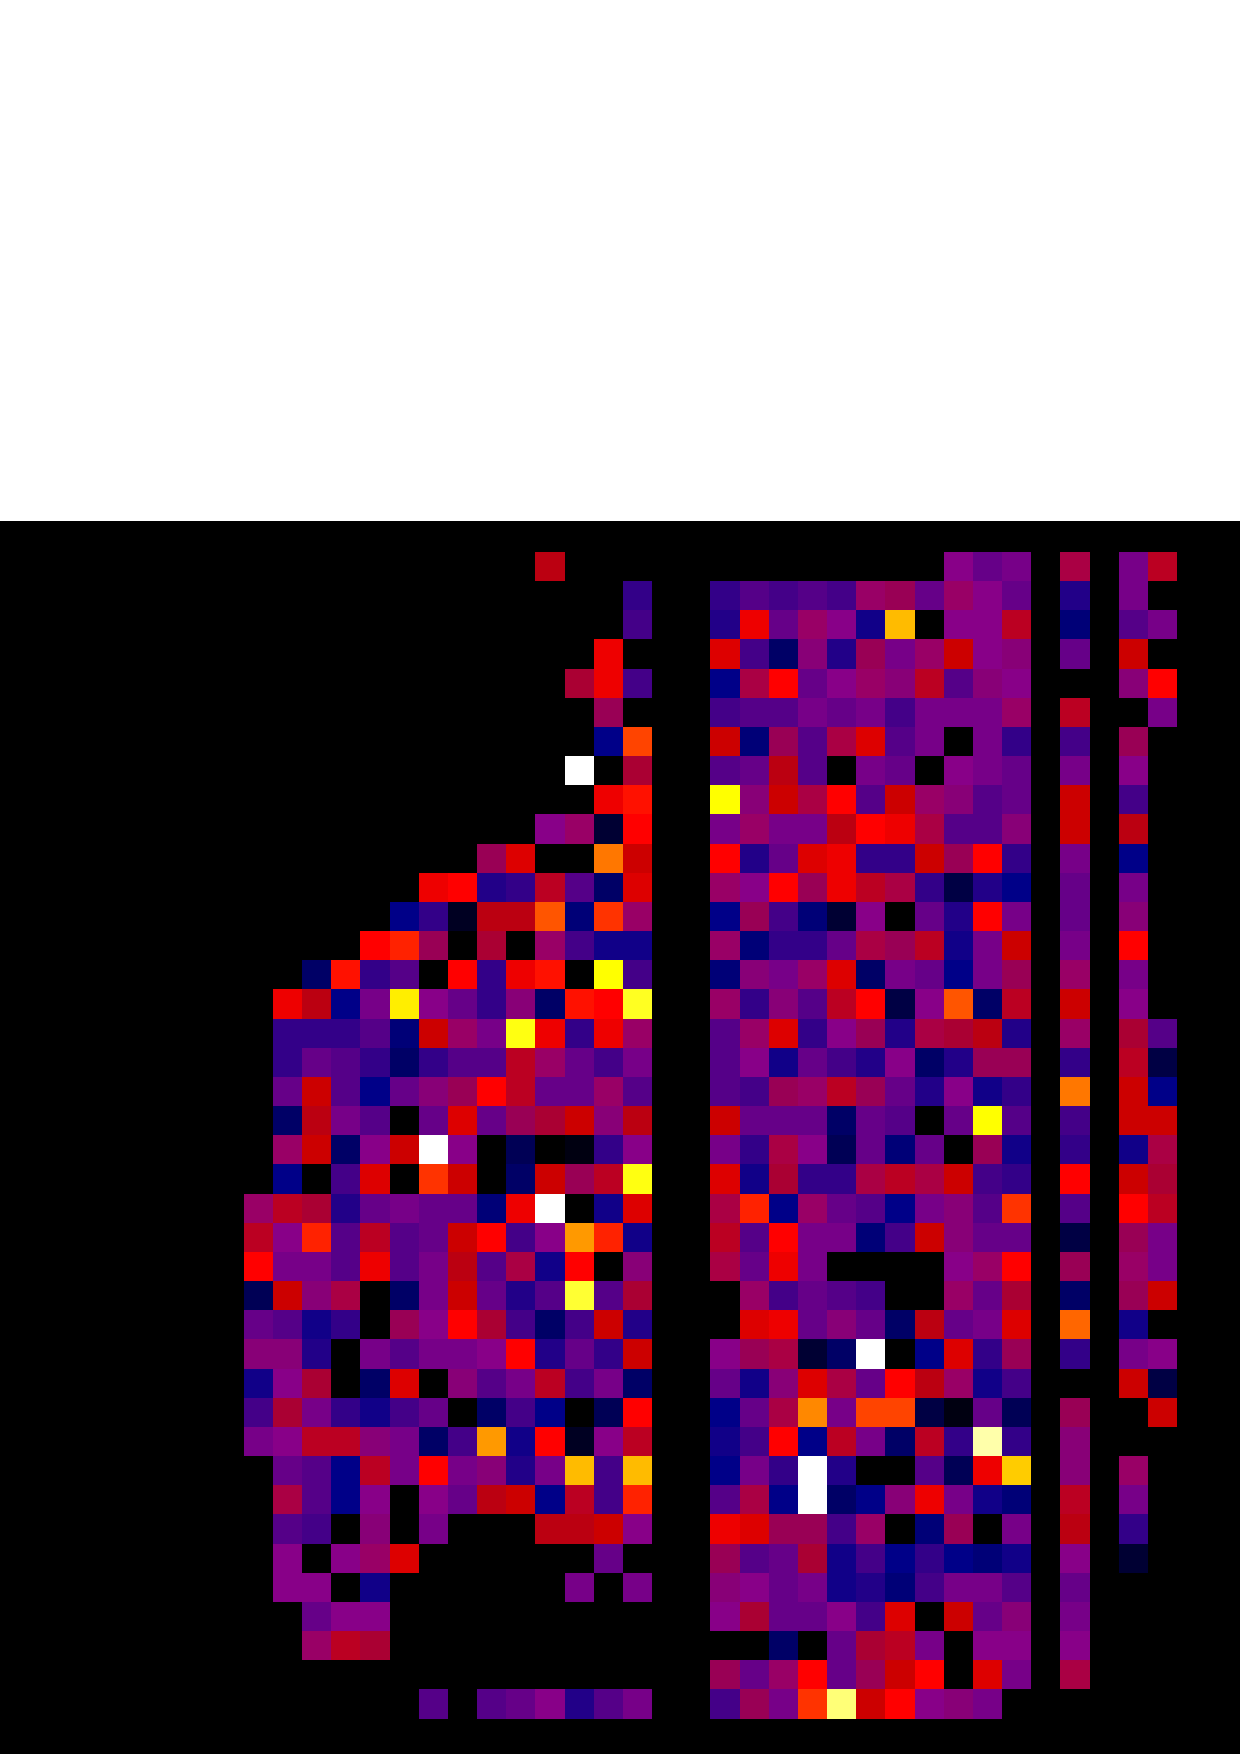
\includegraphics[width=0.45\linewidth]{sc19_conbsl_collapse}
\hspace{0.03\linewidth}
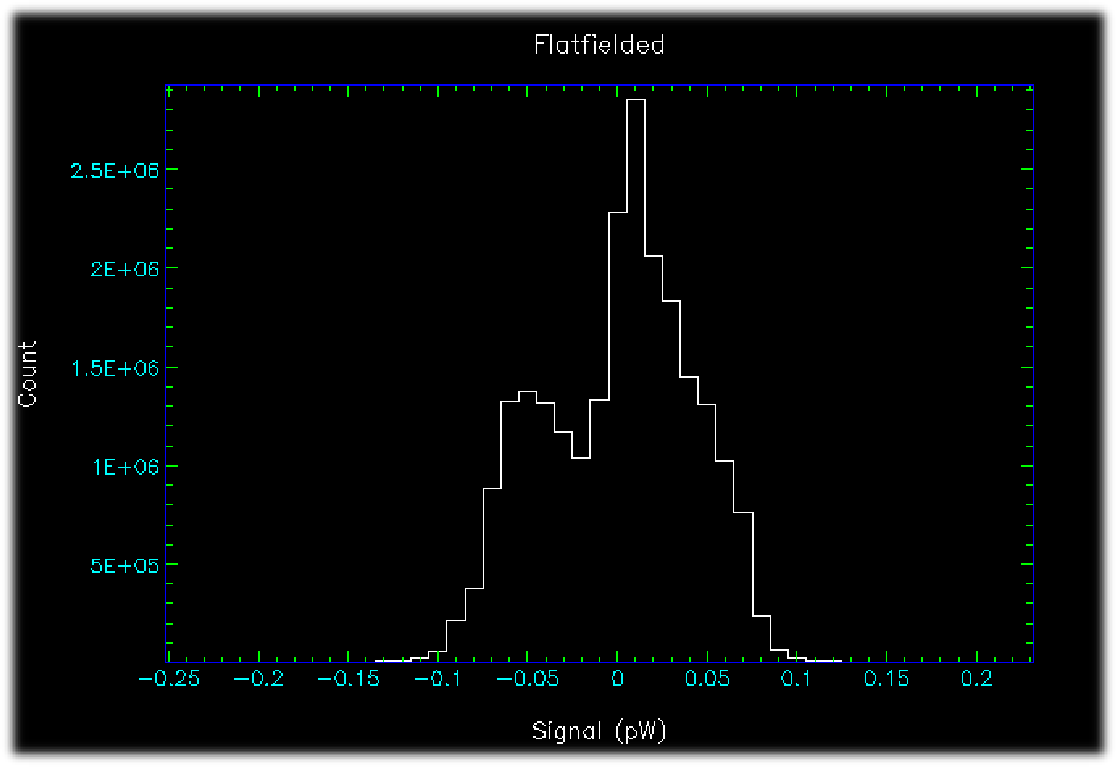
\includegraphics[width=0.45\linewidth]{sc19_bsl_histogram}
\caption{\textsl{left:} Mean signal in DC-removed time-series;
         \textsl{Right:} Histogram of values in DC-removed time series }
\label{fig:conbslcollapse}
\end{center}
\end{figure}

\subsection{\xlabel{spikesteps}Spikes and Steps}
\label{sec:spikesteps}

However, there are still significant outliers: the minimum and maximum
pixel values are \about8.1 and 3.4, respectively. Using \gaia\ to examine
the time series in the DC-subtracted cube reveals remaining data issues as
shown in the Fig.~\ref{fig:timeseries}.

\begin{figure}[ht]
\begin{center}
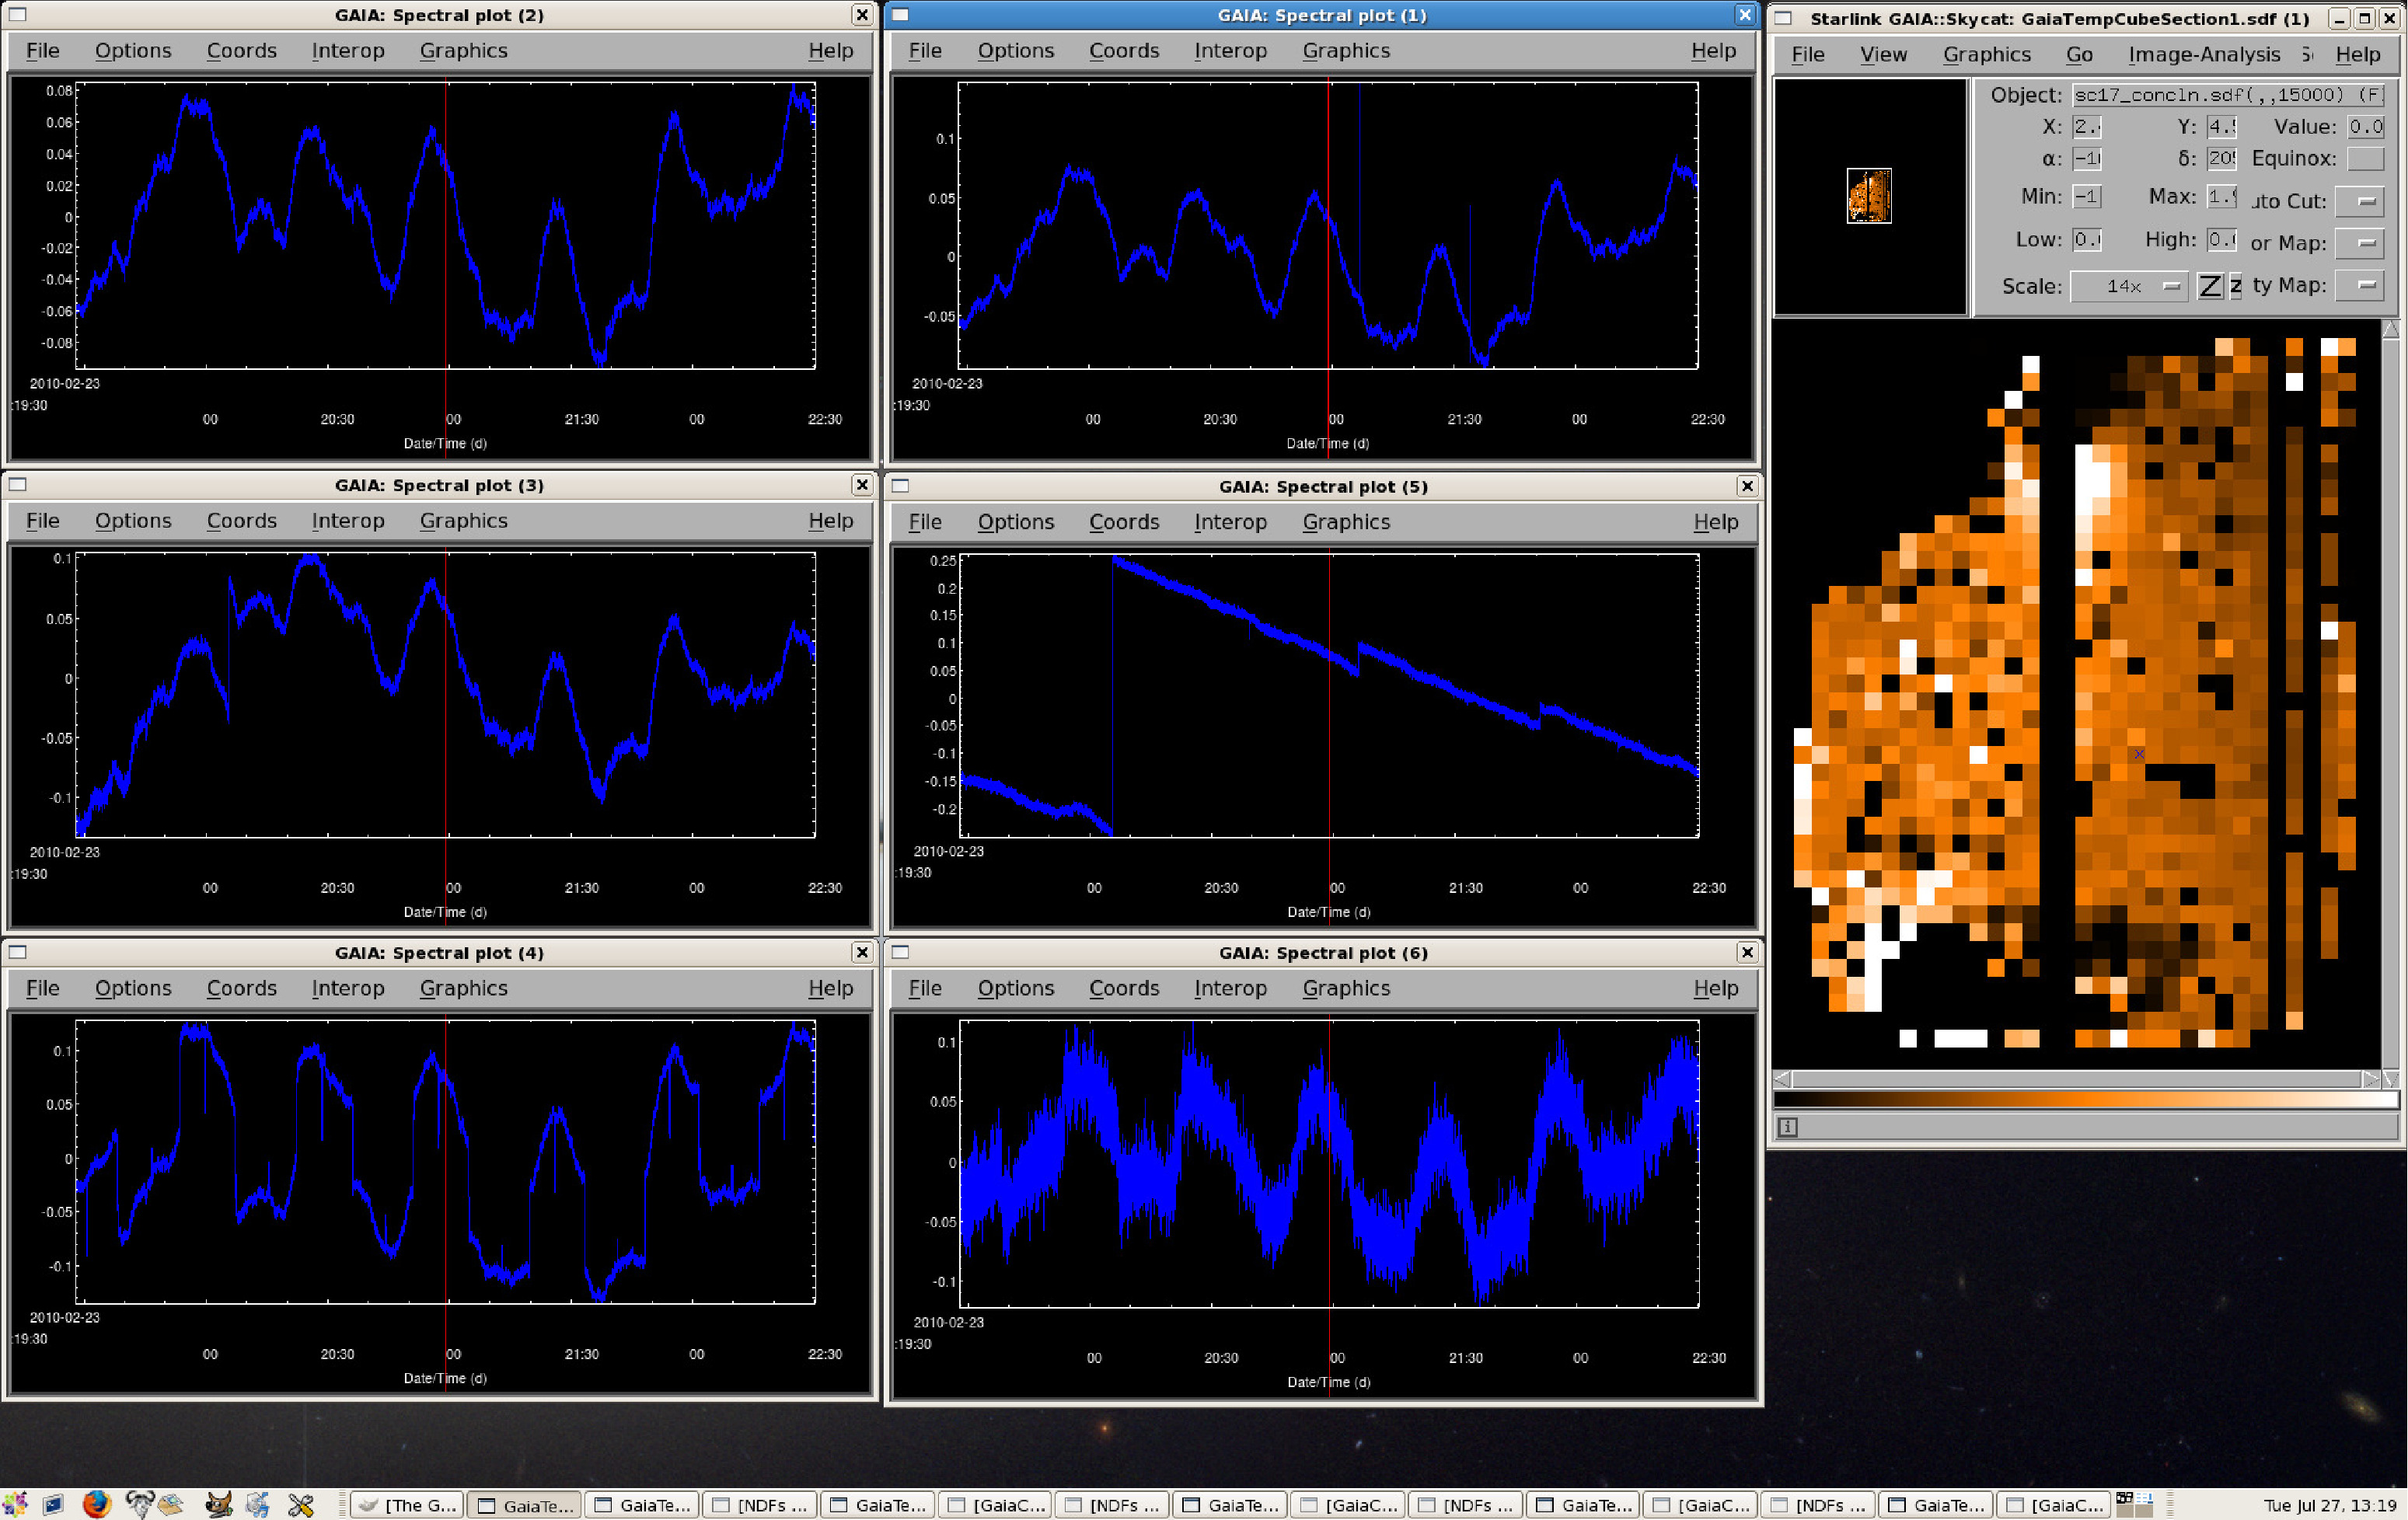
\includegraphics[width=1.0\linewidth]{sc19_timeseries}
\caption{Example time series in the DC-corrected data set showing
spikes, steps, and noisy bolometers. The dominant common-mode signal is
a variation due to a 30~s temperature cycle in the dilution fridge.
\textsl{Top-left:} a bolometer with a typical time
series. Variations due to the 30~s fridge oscillation are
obvious. Since all bolometers share this oscillation it is a
`common-mode' signal, but the amplitude may vary for different
bolometers.
\textsl{Top-right:} a bolometer with spikes in the time
series. \textsl{Middle-left:} a bolometer with a moderate `step'. Steps
can be introduced by the bias for that bolometer `rolling-over' as it
reaches its limit. During the S2SRO the instrument software that flags
these events was not active.
\textsl{Middle-right:} a bolometer with a large step.
\textsl{Bottom-left:} a bolometer with multiple steps and
spikes.
\textsl{Bottom-right:} a `noisy' bolometer. }
\label{fig:timeseries}
\end{center}
\end{figure}

\clean\ is quite efficient in finding steps, but its spike removal is
of limited effectiveness in the presence of a strong common-mode
signal.  As an example \clean\ was re-run with the following
configuration file:\footnote{(These parameters are explained in
  \smurfsun\ (or run \texttt{`smurfhelp makemap config'} or
  \texttt{`smurfhelp sc2clean config'}).}

\begin{terminalv}
% cat my_sc2clean.def
order = 1
dcfitbox = 30
dcthresh = 25.0
fillgaps = 1
dcsmooth = 50
dclimcorr = 0
flagstat = 0
spikethresh = 5
spikebox = 50
noiseclip = 4.0

% sc2clean sc17_con sc17_concln config=^my_sc2clean.def
\end{terminalv}

The results were that \clean\ left the time series of the top two
plots in Fig.~\ref{fig:timeseries} unchanged, i.e.\ the common-mode
variation was too large to cause the spikes in the right time series
to be flagged. \clean\ completely flagged the two time series on the
bottom row as bad. It did an excellent job correcting for the steps in
the middle row time series, as shown in Fig.\ \ref{fig:stepcorrectcf}.

\begin{figure}[ht]
\begin{center}
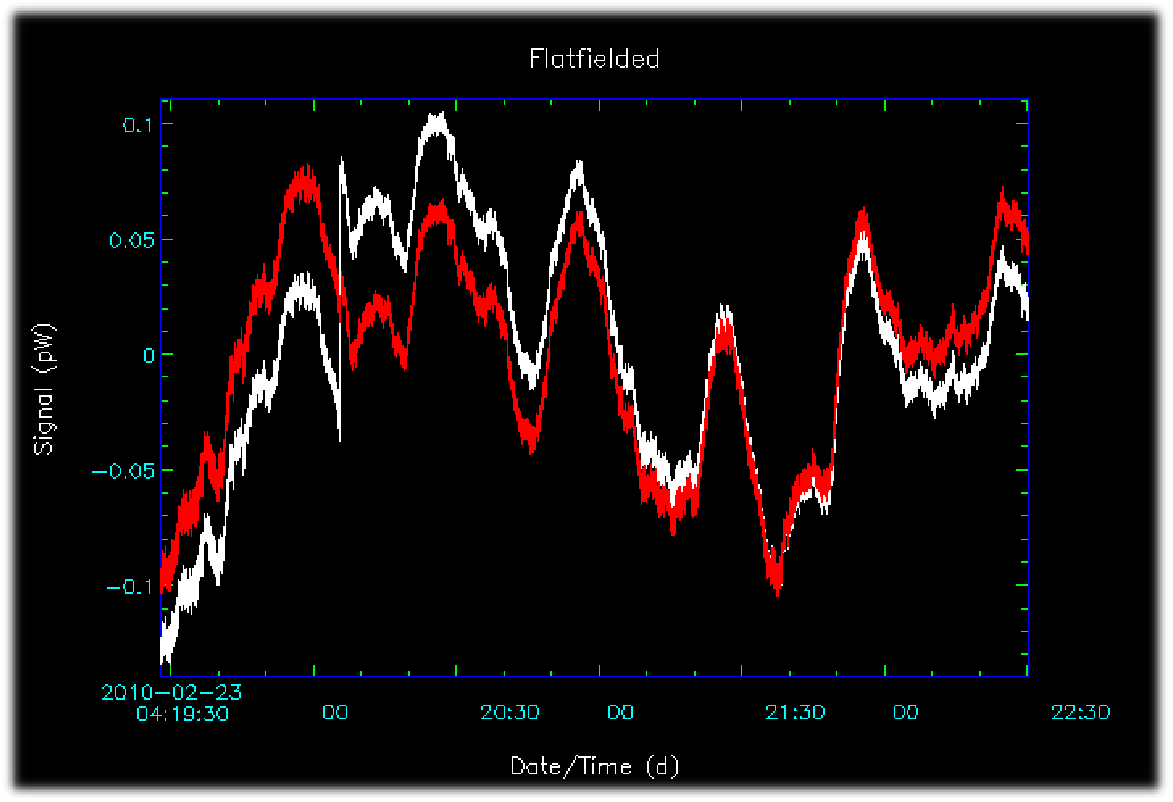
\includegraphics[width=0.45\linewidth]{sc19_sc2clean_13_31}
\hspace{0.03\linewidth}
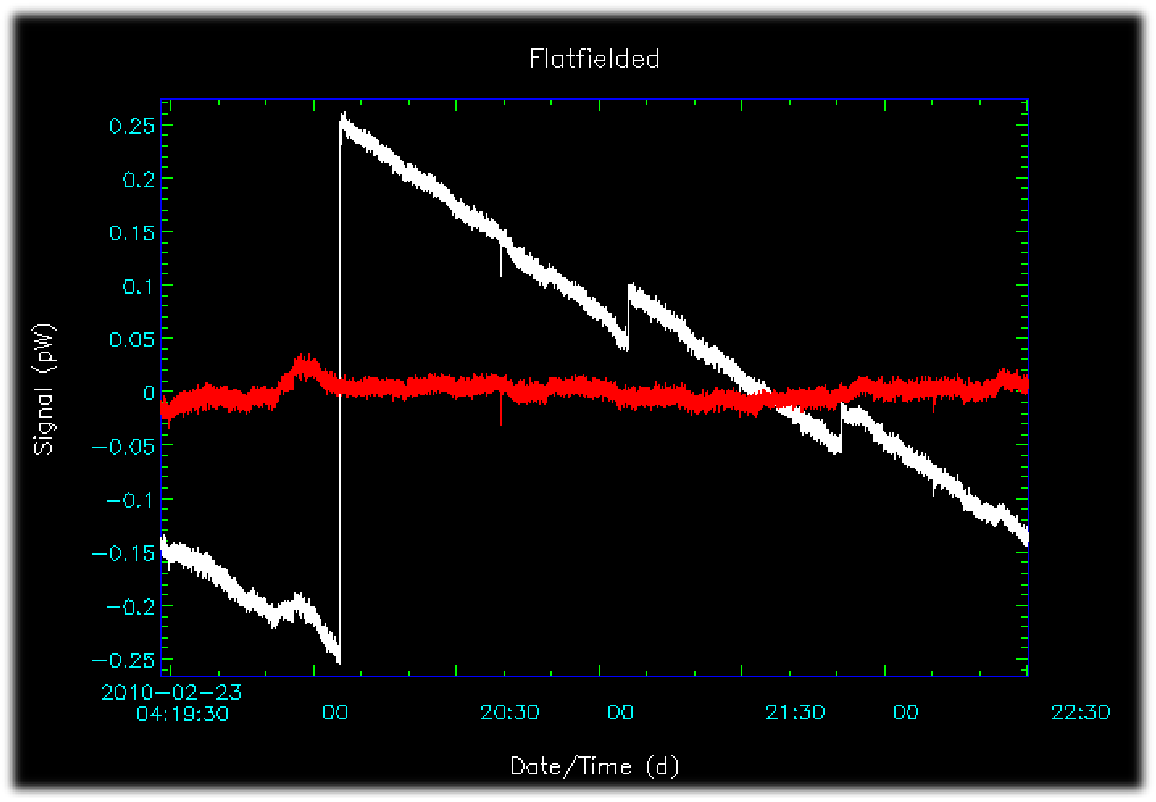
\includegraphics[width=0.45\linewidth]{sc19_sc2clean_16_33}
\caption{Original (white) and sc2clean step-corrected (red) time series.}
\label{fig:stepcorrectcf}
\end{center}
\end{figure}

\subsection{\xlabel{commonmode}Common Mode Signal}
\label{sec:commonmode}

To investigate features of the time series further one needs to get
rid of the dominant common-mode signal. Most of the variation seen is
due to a 30-sec temperature cycle of the dilution fridge. This cycle
affects the biasing of the bolometers and, in effect, varies the
zero-level of each on that time-scale. There are various ways to
remove this signal for quick inspection of the data, but here are two.
Again, please be reminded that the aim here is not to reduce the data
for map-making, but to illustrate characteristics of the data set.

\textsl{Method 1:} The simplest method is to mimic the action of the SMO module
of the DIMM: subtract the median in a sliding box from the time
series.

\textsl{Method 2:} Use the DIMM to subtract the common-mode signal and
export the models for further inspection. The common-mode is captured
by the \texttt{COM}, \texttt{GAI}, and \texttt{FLT} models as
\texttt{GAI*COM+FLT}.

\subsubsection{\xlabel{method1}Method 1}
\label{sec:method1}

The first method can be implemented rather simply using `block'
although the calculation of the sliding medians will take quite
long. Since the time series corresponds to a path across the sky, this
obviously suppresses any structures larger than the path corresponding
to the box. However, it is a very efficient method to flatten the time
series (including steps which can change into spikes) to allow an easy
statistical analysis of the intrinsic noise characteristics of
bolometers.  This `harsh selection' method may have merits for the
analysis of point-source fields, but be aware that the DIMM
in general will leave significantly more `baseline' systematics in the
time-series.

\begin{terminalv}
(csh)
set file = sc17_conbsl
echo "Subtract time-series block median"
block estimator=median in=${file} out=${file}_block \
      wlim=0 box='[1,1,200]'
sub ${file} ${file}_block ${file}_subblk
\end{terminalv}

A block-size of 200 corresponds to 1 sec of data, which can be related
to a spatial size through the maximum scanning speed
e.g.\ 120\,arcsec/sec. Remember though that the telescope spends a large
fraction of the time at lower speeds either accelerating or
decelerating. In fact, a block-size of 200 largely removed the signal
from CRL\,618 from this data set!

\begin{figure}[ht]
\begin{center}
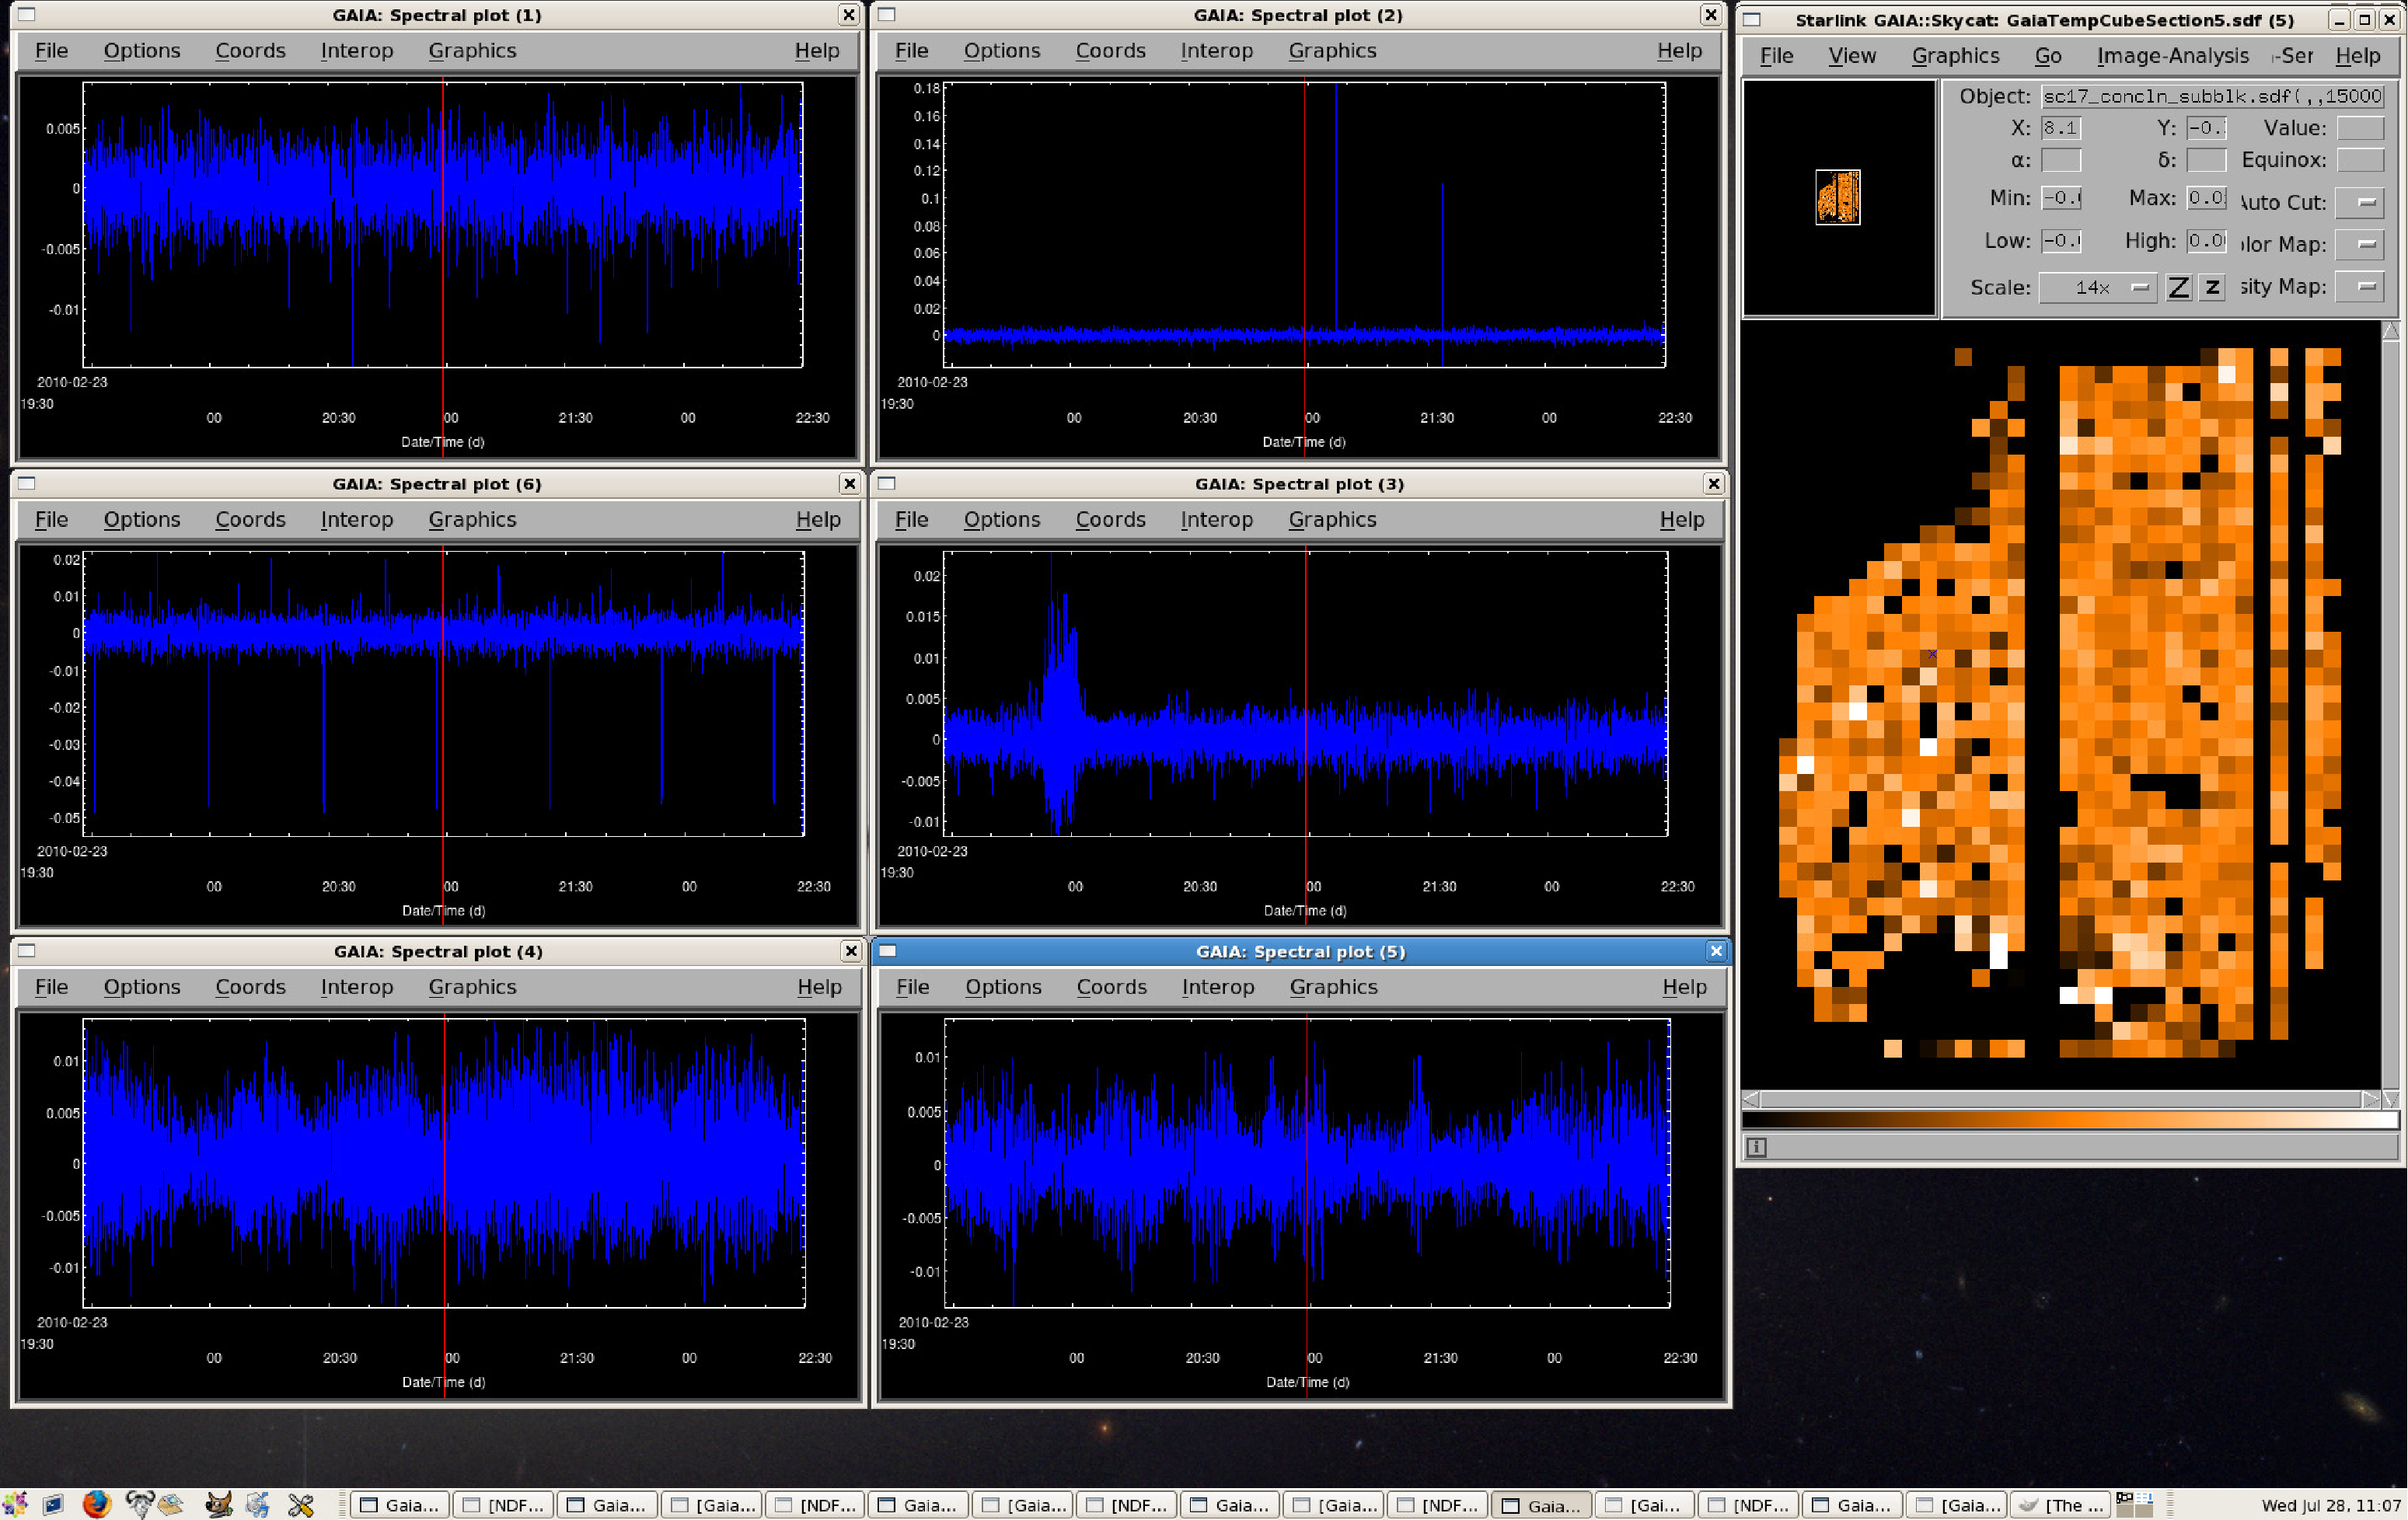
\includegraphics[width=1.0\linewidth]{sc19_timeseries2}
\caption{Example time series in the block-median common-mode
subtracted data set high-lighting intrinsic noise issues that can be
seen in bolometers. The top-left time series is the same as the
top-left time series in figure Fig.~\ref{fig:timeseries}}
\label{fig:timeseries2}
\end{center}
\end{figure}

An inspection of resulting file shows very flat time series. The
top-left panel in the Fig.~\ref{fig:timeseries2} shows a typical
time-series after removal of a sliding median. The next two panel show
time-series with negative and positive spikes. The middle-right panel
shows a bolometer with an increased noise during part of the scan. The
next two panels show bolometers with an uneven noise performance. Note
that the DIMM will \textsl{not} specifically handle these
issues, apart from de-spiking and an iterative clip of bolometers
based on their overall noise level.  It also is the case the residual
variations remaining after a common-mode subtraction often are of a
similar or larger level: the sliding-median method allows one to zoom
in on the noise characteristics of individual bolometers and possibly
derive a bad-bolometer map for use with the DIMM (many SCUBA-2
tasks accept a `bbm').

A word of caution: at the high scanning speeds, point-like sources
will look as spikes in the time series. At 120\,arcsec/sec it takes the
telescope at least 10 samples to cross the 45\micron\ beam. However, at
600\,arcsec/sec (as may be used for large scan maps), the crossing happens in
barely more than 2 samples!

One can attempt to further identify problematic bolometers by,
for example, calculating the rms of each time series, but that falls outside
the scope of this document:

\begin{terminalv}
collapse ${file}_block ${file}_block_rms estimator=rms \
         axis=3 variance=false wlim=0.0
\end{terminalv}

\subsubsection{\xlabel{method2}Method 2}
\label{sec:method2}

Method 2 is to use the DIMM to derive the common mode signal. The
common-mode signal will be \texttt{GAI*COM+FLT}. There are a few gotchas to
keep in mind though (note that some of these may change as the program
gets further optimized):

\begin{itemize}
\item The DIMM will do a \clean\ in a preprocessing step
  which makes it hard to compare the models to the original file. At
  the least do an external DC removal first (as outlined above).  Or
  do the \clean\ as an external step and switch off all \clean\
  parameters in the dimmconfig file submitted to the DIMM.

\item The DIMM will add padding on either side of the time series but
  not remove it from the models before writing them out. There
  currently is a bug that requires one to use `setorigin' to properly
  align these cubes with the original one.

\item The current \texttt{FLT} model will apodize (i.e.\ smoothly
  reduce the ends of the time series to zero; these ends are not used
  for the mapmaking). The apodization is needed for \texttt{FLT}'s
  current FFT, but a non-apodizing FFT method is under development.

\item \param{com.notfirst} regulates whether the \texttt{COM} model is
  run during the first iteration. If set to 1, most of the dominant
  fridge-related variations will end up in the \texttt{FLT} model. A
  priori this is not a problem as far as removing the signal is
  concerned, but the \texttt{FLT} model works on each time series
  individually i.e.\ does not really derive a common-mode.

\item Related to the previous point, if the fridge variations end up
  in the \texttt{FLT} model, the \texttt{GAI} model will not really
  show the gain variation across the bolometers, since the
  \texttt{COM} model in that case will only contain the residual
  common-mode variation (often dominated by ringing artefacts from
  \texttt{FLT}'s FFT). i.e.\ for this exercise we want to make sure
  that \texttt{com.notfirst=0}.

\item The first plane of the \texttt{GAI} model has the multiplicative
  term but it is distributed around the median (or mean) gain rather
  than a value of 1 due to the way that the \texttt{GAI} and
  \texttt{COM} models have been implemented. i.e.\ divide the gain map
  by its median in order to get a value distributed around 1. However,
  note a subtlety: the gain of each bolometer in principle should have
  been fitted and accounted for by the flat field.  Any gain differing
  from 1 in the \texttt{GAI} model can be interpreted as either a poor
  flat-field fit, the gain being variable, or some basic bolometers
  characteristics, e.g.\ their individual resistances, not (yet) being
  accounted for sufficiently.
\end{itemize}

For example, for these observations of CRL\,618 modify the
\texttt{dimmconfig\_bright\_compact.lis} configuration file as
follows. Given that, at the time of writing, the FLT model apodizes,
it has been left out.

\emph{A reminder: this exercise aims at showing data features and
\textbf{not} at showing how well the DIMM can handle these. For the
latter one would want to run the DIMM with all its features
enabled.}

\begin{small}
\begin{terminalv}
^$STARLINK_DIR/share/smurf/dimmconfig_bright_compact.lis

numiter = 3                        # Just run a few iterations
modelorder = (com,gai,ast)         # Just do common mode part
exportndf = (com,gai,ast,res)      # Write models out
itermap = 1                        # Create map for each iteration
com.gain_box = 600000              # Single gain map for whole spectrum
order = 0                          # Allow for DC level adjustments
dclimcorr = 0                      # No correlated step detection/correction
com.notfirst=0                     # Make sure that COM is run before FLT
\end{terminalv}
\end{small}

The above file exports all relevant models. It produces a moderately
smoothed common mode time series and a single gain component for the
whole observation. A script that handles combines the output models
into a common-mode and common-mode subtracted cube is appended at the
end of the document. It actually gives us three useful files to look
at: the derived common-mode signal \texttt{(\_commode)}, the relative
gains of the bolometers \texttt{(\_gain)}, as well as a common-mode
subtracted cube \texttt{(\_astres)}.

\begin{myquote}
\textsl{The common-mode reduction script is appended at the end of this document.}
\end{myquote}

\begin{figure}[ht]
\begin{center}
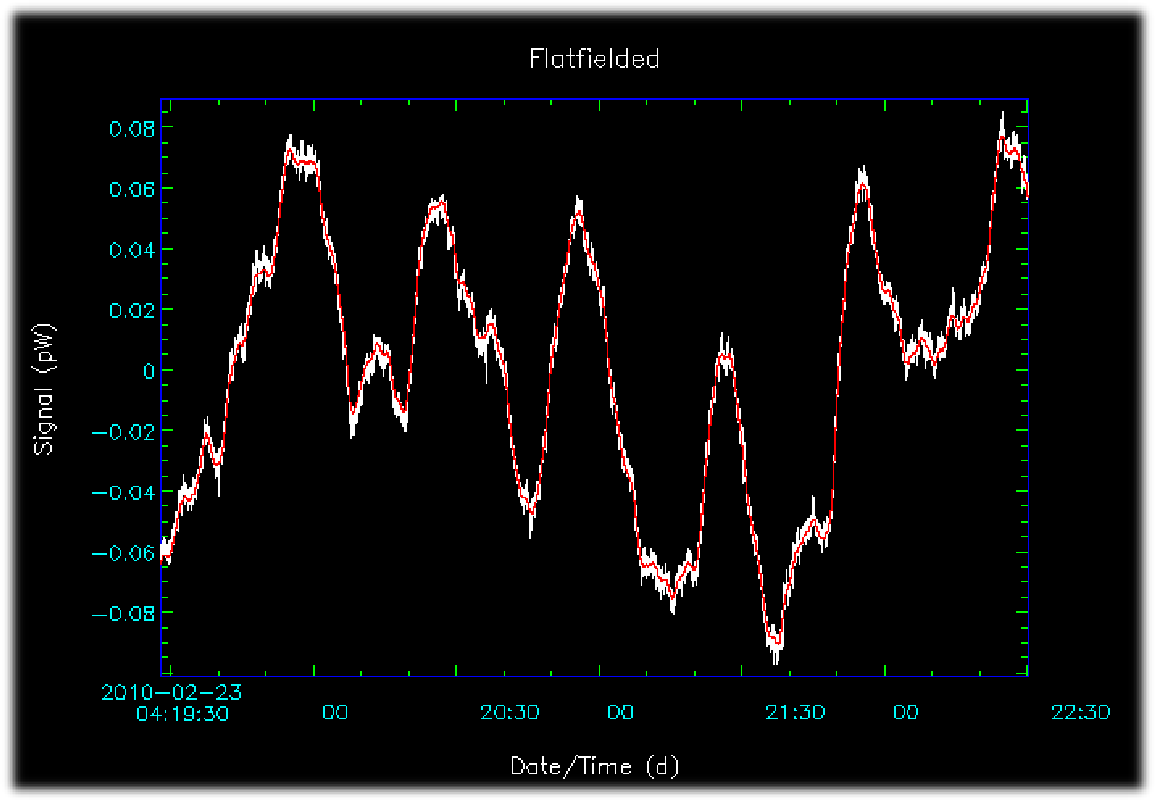
\includegraphics[width=0.45\linewidth]{sc19_dimm_common_mode}
\caption{Example time series (white) and the derived
common-mode signal (red).  This time series is the same as the
top-left time serie in Figs.~\ref{fig:timeseries} and \ref{fig:timeseries2}}
\label{fig:dimmcommonmode}
\end{center}
\end{figure}

Fig.~\ref{fig:dimmcommonmode} shows a typical time series with the
fitted common-mode signal.

The input cube to makemap had 812 `good' bolometers, the derived gain
map 651: makemap has flagged an additional 161 bolometers as bad.  A
quick inspection of the masked bolometers shows that the majority have
steps, increased noise, or multiple spikes.  The gain map itself
ranges from 0.44 to 1.89 and a histogram shows that of the 651
unflagged bolometers 593 (\about90 per cent) are within a range of
[0.75,1.25] and 622 within [0.65,1.35]. To some degree this range
indicates that for the S2SRO data the flat field \textsl{in practice}
was in general not very accurate or stable probably due to one or more
of the aforementioned reasons.

\begin{figure}[ht]
\begin{center}
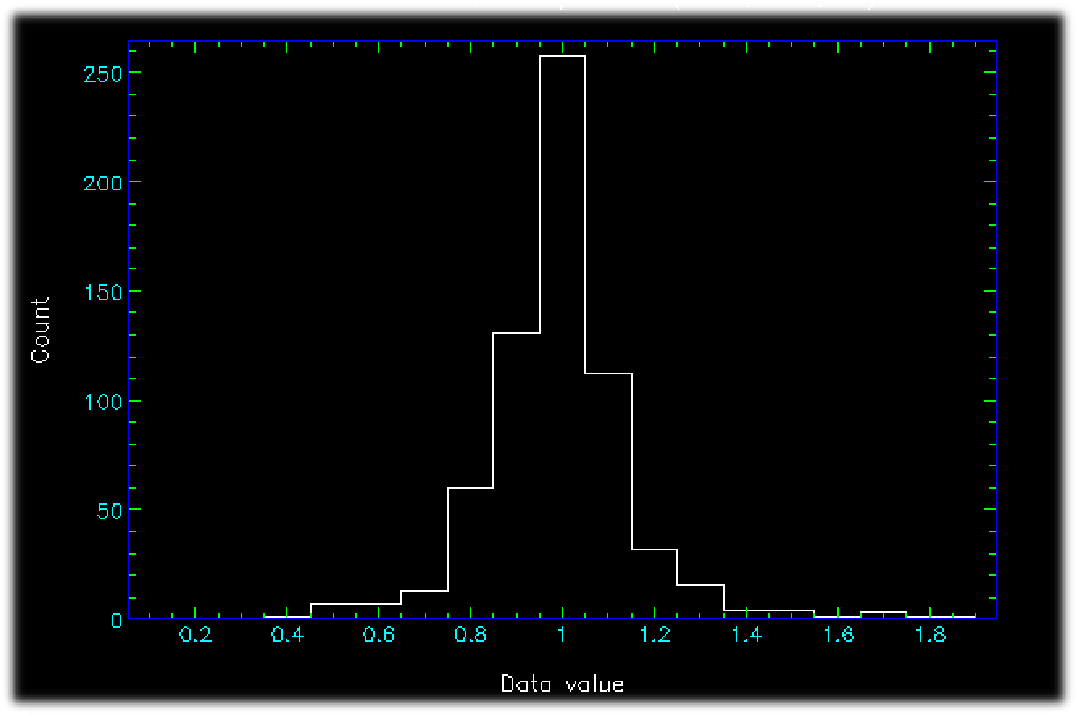
\includegraphics[width=0.45\linewidth]{sc19_gain_histogram}
\caption{Histogram of the bolometer gains as derived by the DIMM
based on their response to the common-mode signal. Note that these
gains are, by default, only used for the subtraction of the common
mode and not for the subsequent gridding into a map.}
\label{fig:gainhistogram}
\end{center}
\end{figure}

For a further analysis one can also e.g.\ collapse the common-mode
subtracted cube over the time-series to calculate the median and rms:

\begin{terminalv}
% collapse ${file}_astres ${file}_astres_median estimator=median \
           axis=3 variance=false wlim=0.0
% collapse ${file}_astres ${file}_astres_rms estimator=rms \
           axis=3 variance=false wlim=0.0
\end{terminalv}

The median \textsl{signal} ranges from $-$33e-04 to 30e-04, with 582
bolometers falling within a range of $-$5e-04 to 5e-04. The median
\textsl{rms} is 3e-03 with a maximum of 14e-03 and 578 bolometers
below a rms of 6e-03 (twice the median).  The three panels in
Fig.~\ref{fig:masks} summarize this information.

\begin{figure}[ht]
\begin{center}
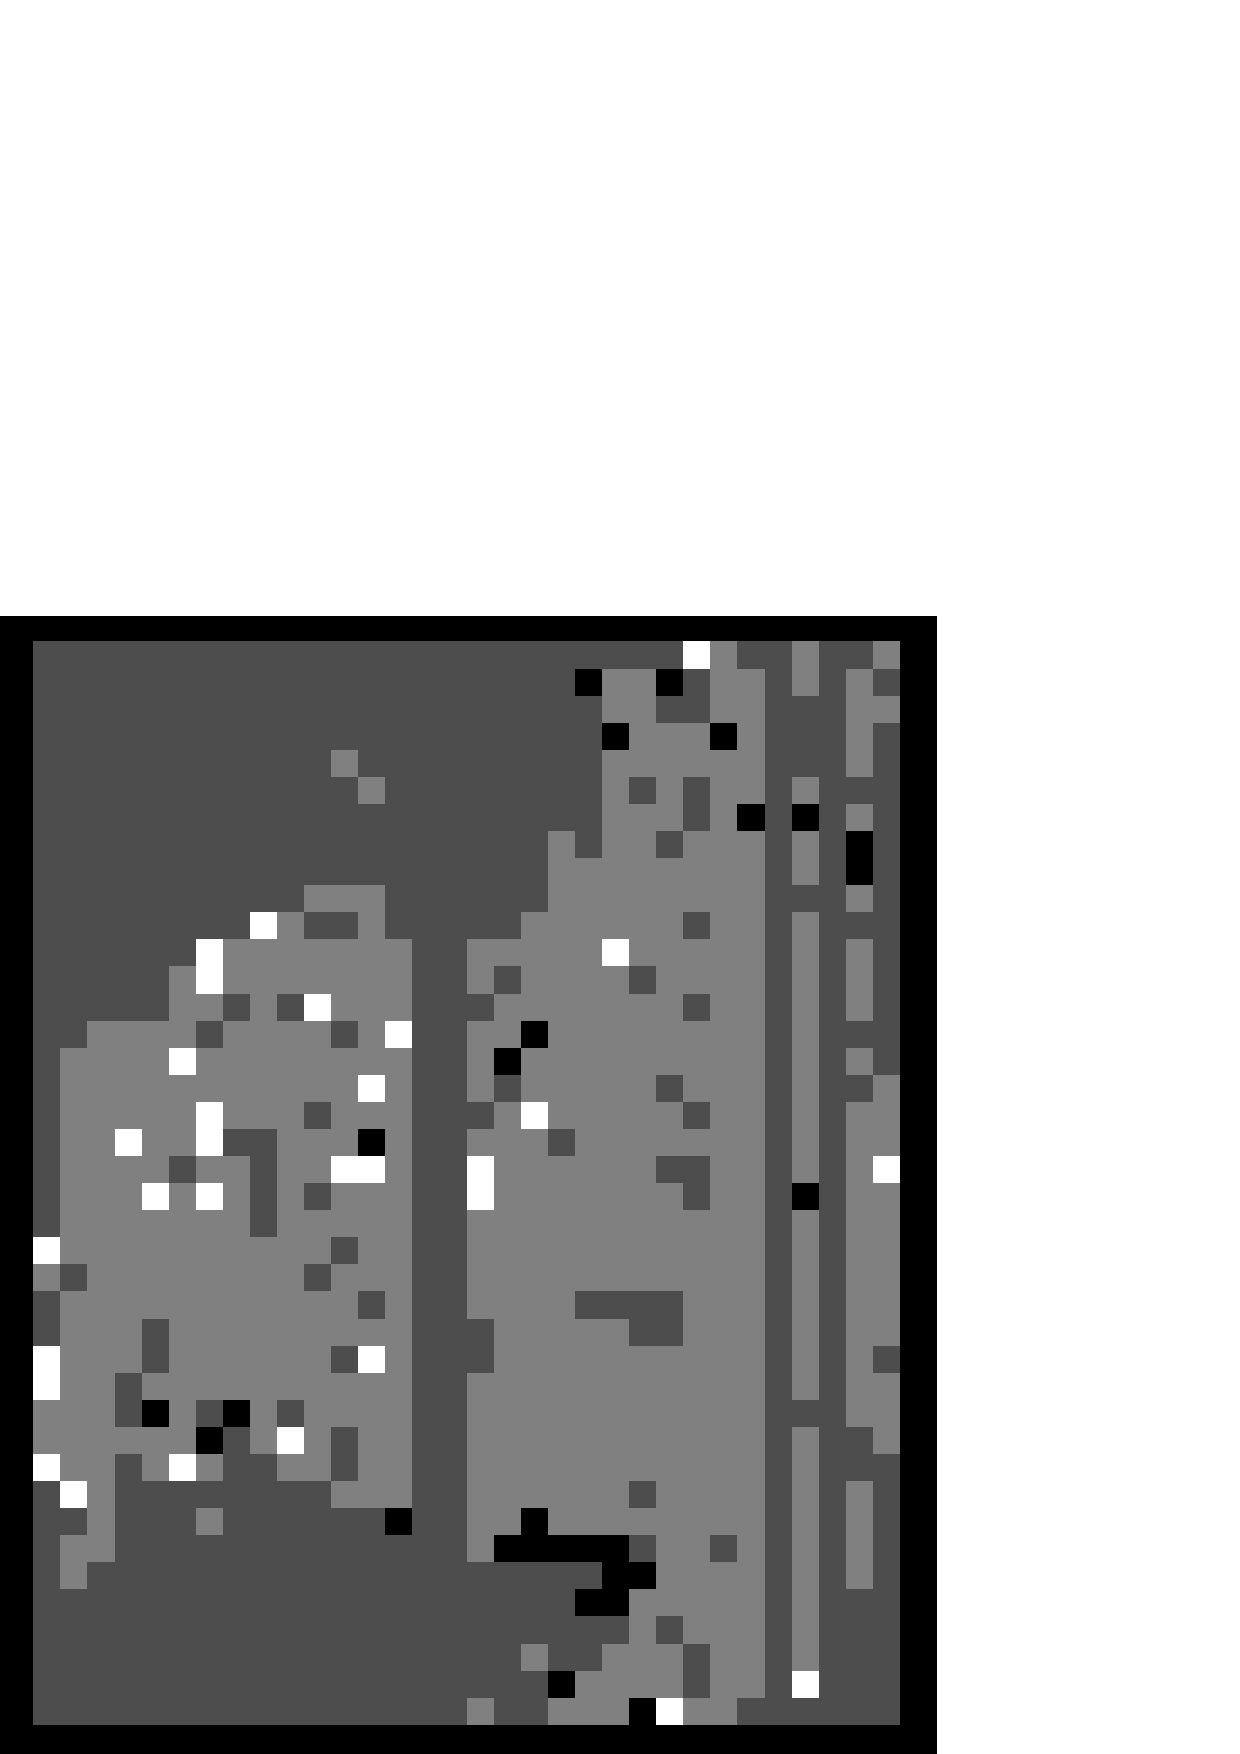
\includegraphics[width=0.30\linewidth]{sc19_conbsl_gainmsk}
\hspace{0.03\linewidth}
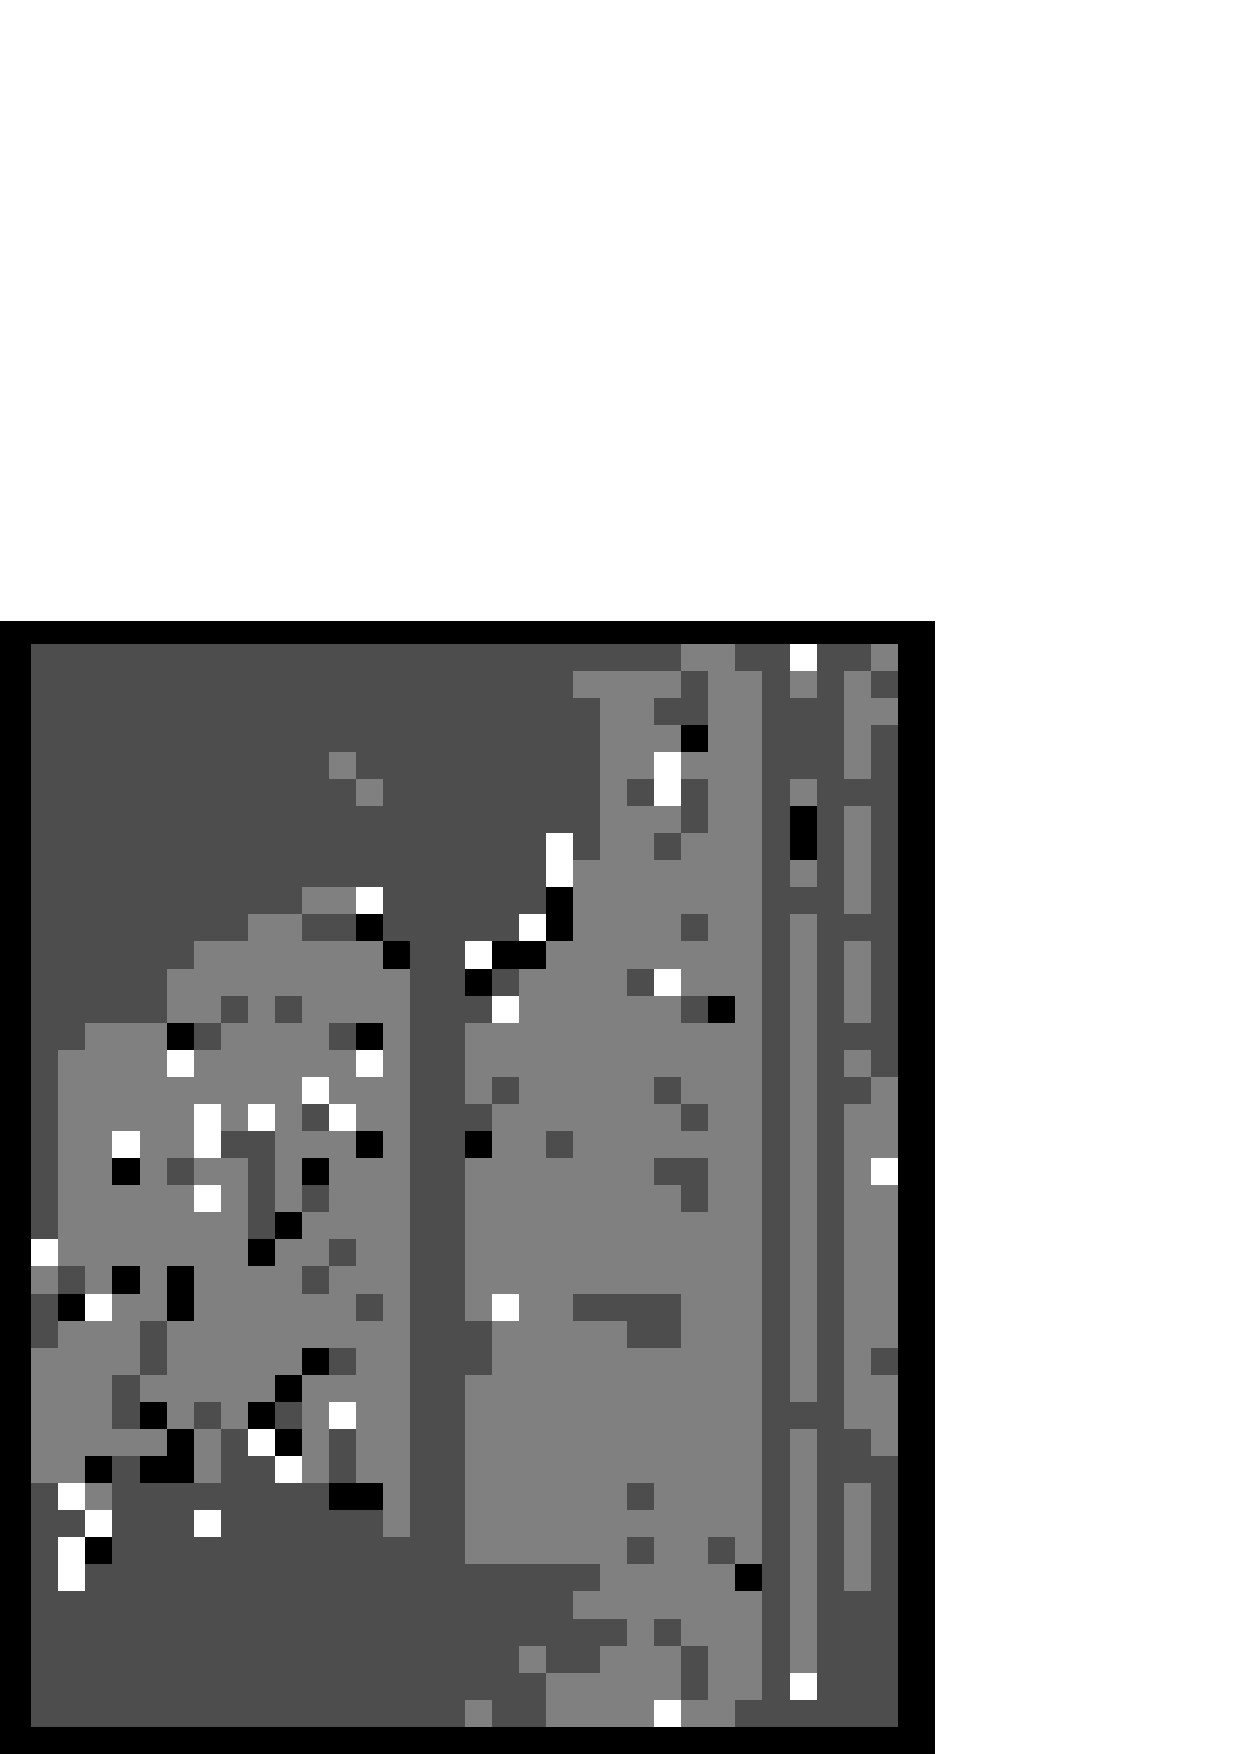
\includegraphics[width=0.30\linewidth]{sc19_conbsl_astres_medianmsk}
\hspace{0.03\linewidth}
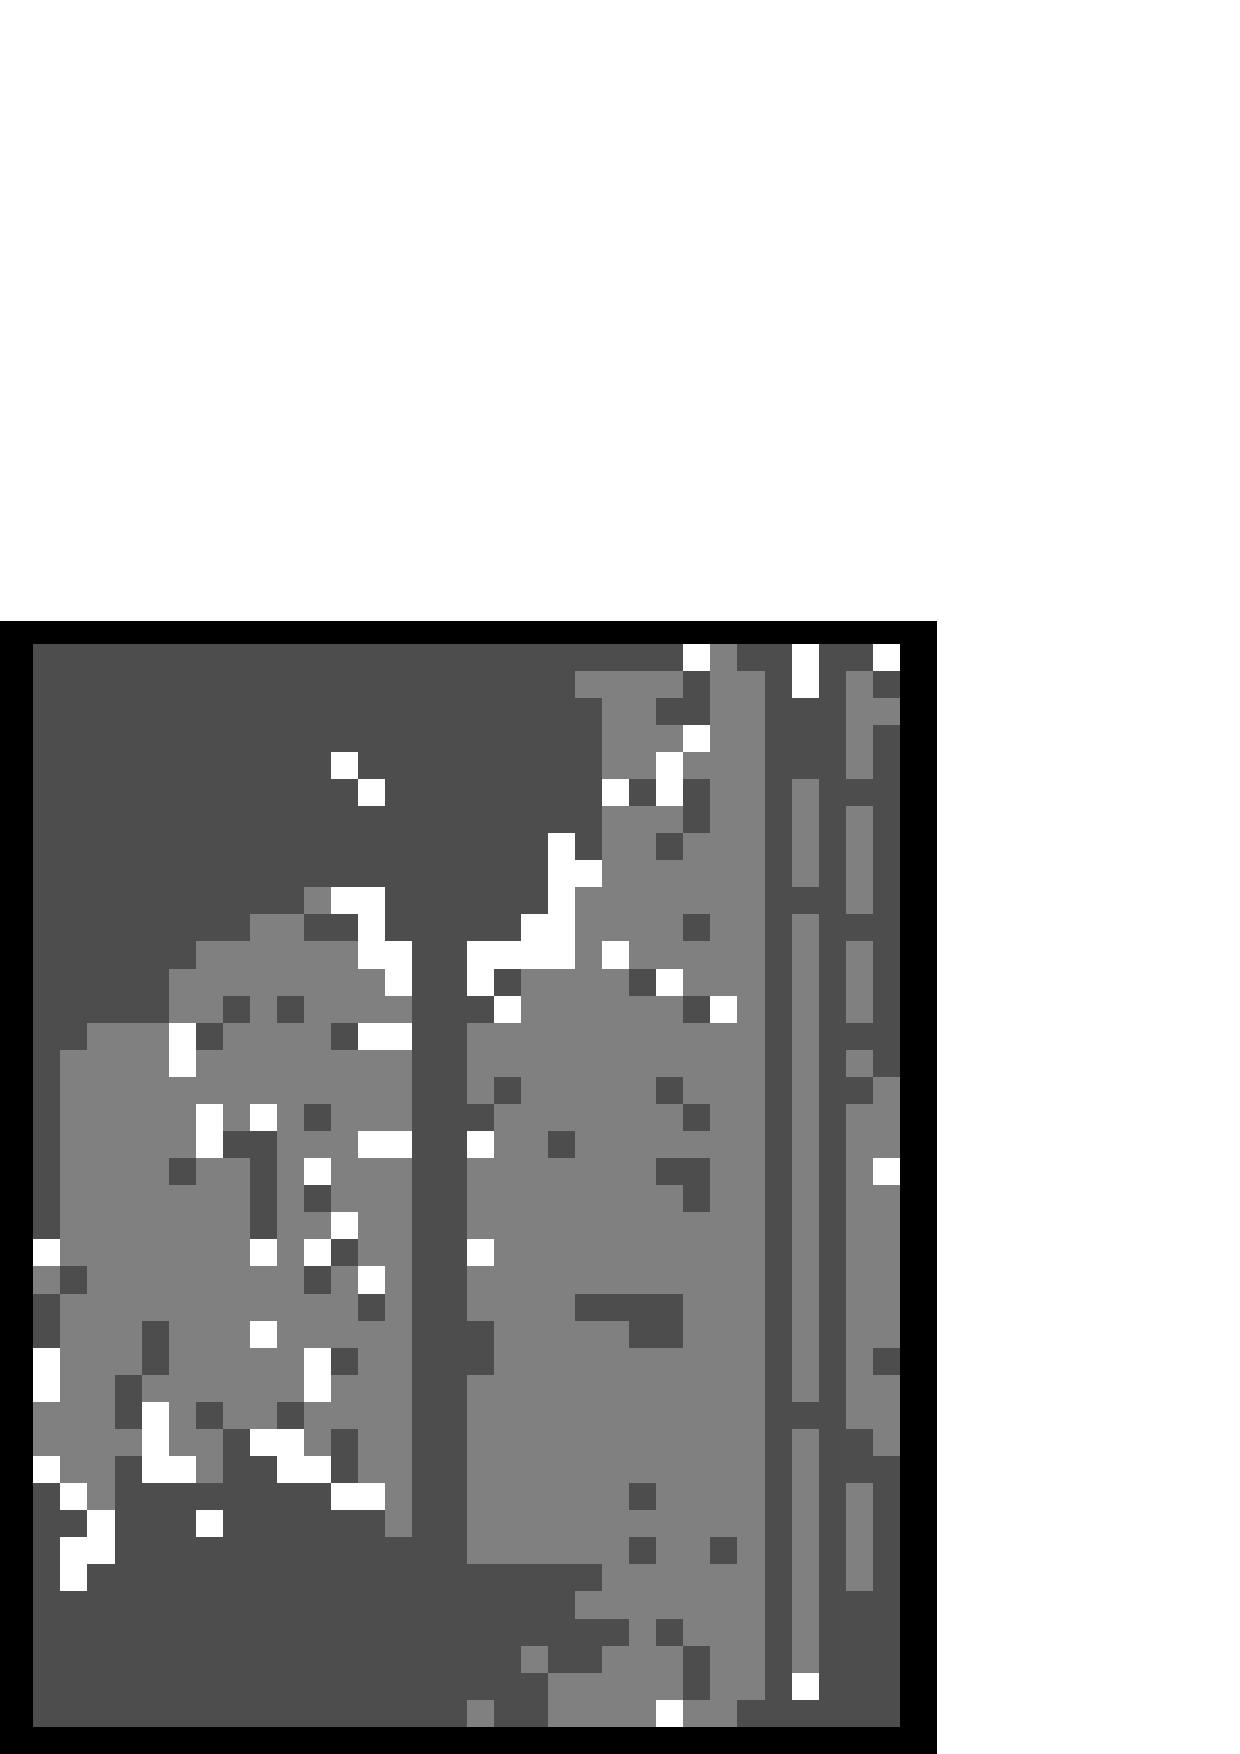
\includegraphics[width=0.30\linewidth]{sc19_conbsl_astres_rmsmsk}
\caption{\textsl{Left:} Gain image: black $<$ 0.75, white $>$ 1.25;
\textsl{Middle:} Common-mode subtracted median: black $< -$5e-04, white $>$ 5e-04
\textsl{Right:} Common-mode subtracted rms: white $>$ 6e-03 (twice the median).}
\label{fig:masks}
\end{center}
\end{figure}

\begin{terminalv}
% thresh ${file}_gain'(,,~1)' temp \
         thrlo=0.75 thrhi=1.25 newlo=0.0 newhi=2.0
% thresh temp ${file}_gainmsk \
         thrlo=1.5 thrhi=0.5 newlo=1.0 newhi=1.0
% thresh ${file}_astres_median'(,,~1)' temp \
         thrlo=-5e-04 thrhi=5e-04 newlo=-1.0 newhi=1.0
% thresh temp ${file}_astres_medianmsk \
         thrlo=5e-04 thrhi=-5e-04 newlo=0.0 newhi=0.0
% thresh ${file}_astres_rms'(,,~1)' temp \
         thrlo=0 thrhi=6e-03 newlo=-1.0 newhi=1.0
% thresh temp ${file}_astres_rmsmsk \
         thrlo=6e-03 thrhi=0 newlo=0 newhi=0
\end{terminalv}

The three maps have a significant subset of `flagged' bolometers in
common.  An inspection of the common-mode subtracted data \texttt{(\_astres)}
shows that many of these bolometers have (multiple) steps that were
not removed by \clean.  Another subset shows variations that don't
seem well modeled by the common-mode signal, although one has be
careful not to mark the signature from CRL\,618 as bad. But even for
bolometers that pass through all the selection `filters' there are
quite a few that still have spikes, steps, or baseline ripples.
Although the mapmaker was deliberately crippled for the above
presentation, further development of the mapping algorithms will be
needed to optimally handle SCUBA-2 data and produce the best possible
maps.

\begin{figure}[ht]
\begin{center}
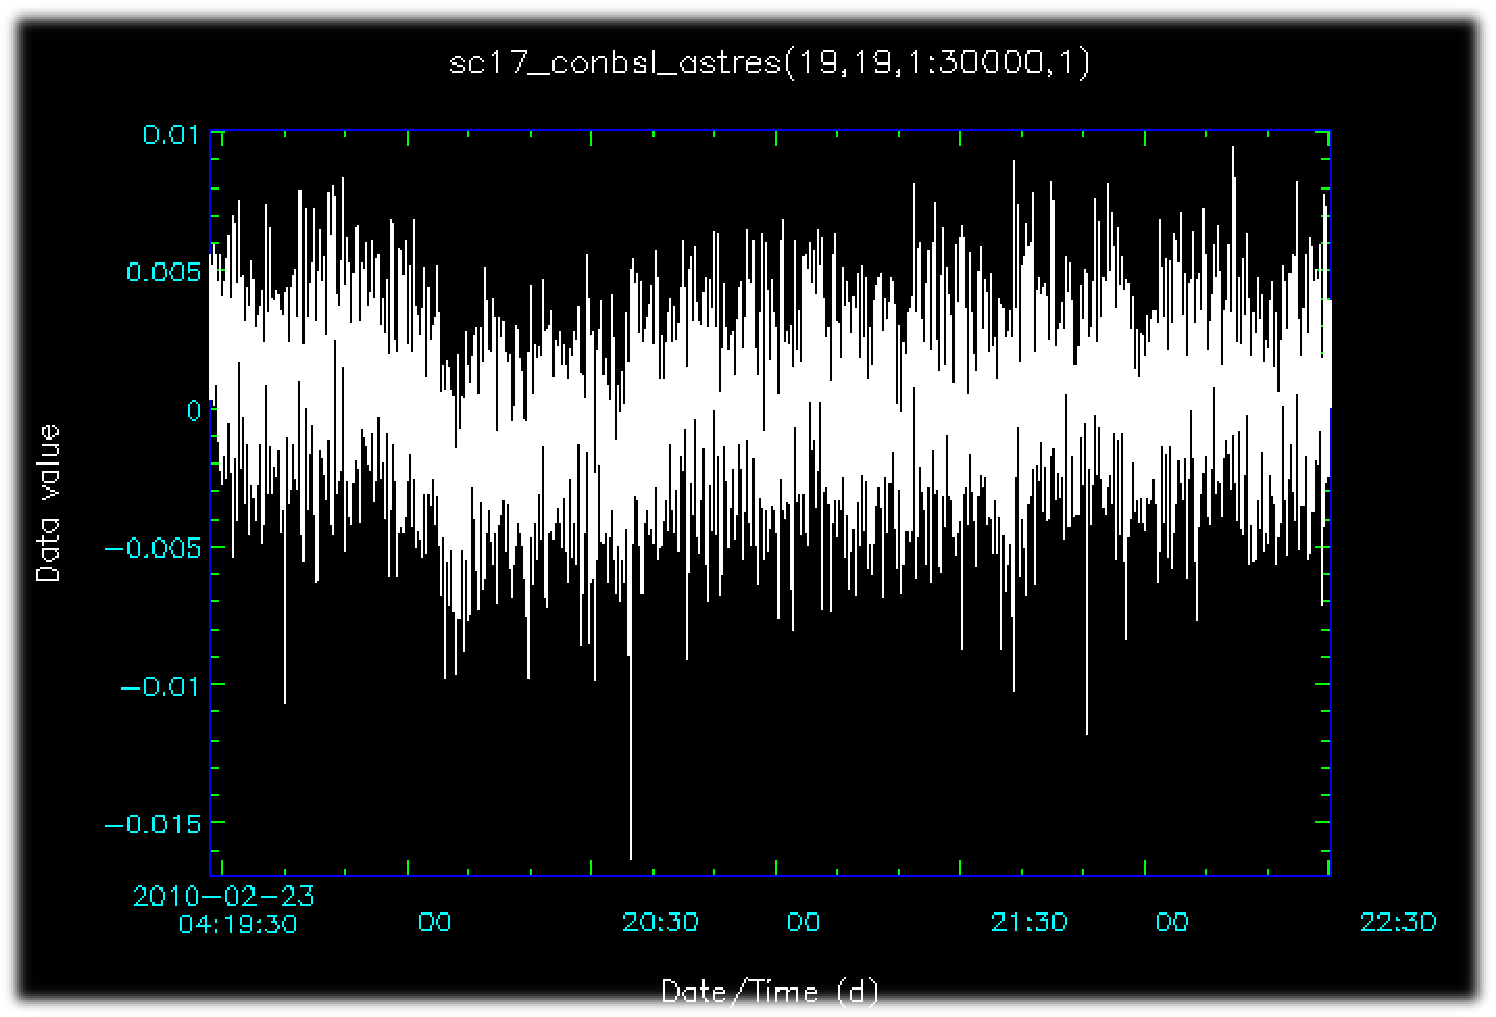
\includegraphics[width=0.30\linewidth]{sc19_conbsl_astres_19_19}
\hspace{0.03\linewidth}
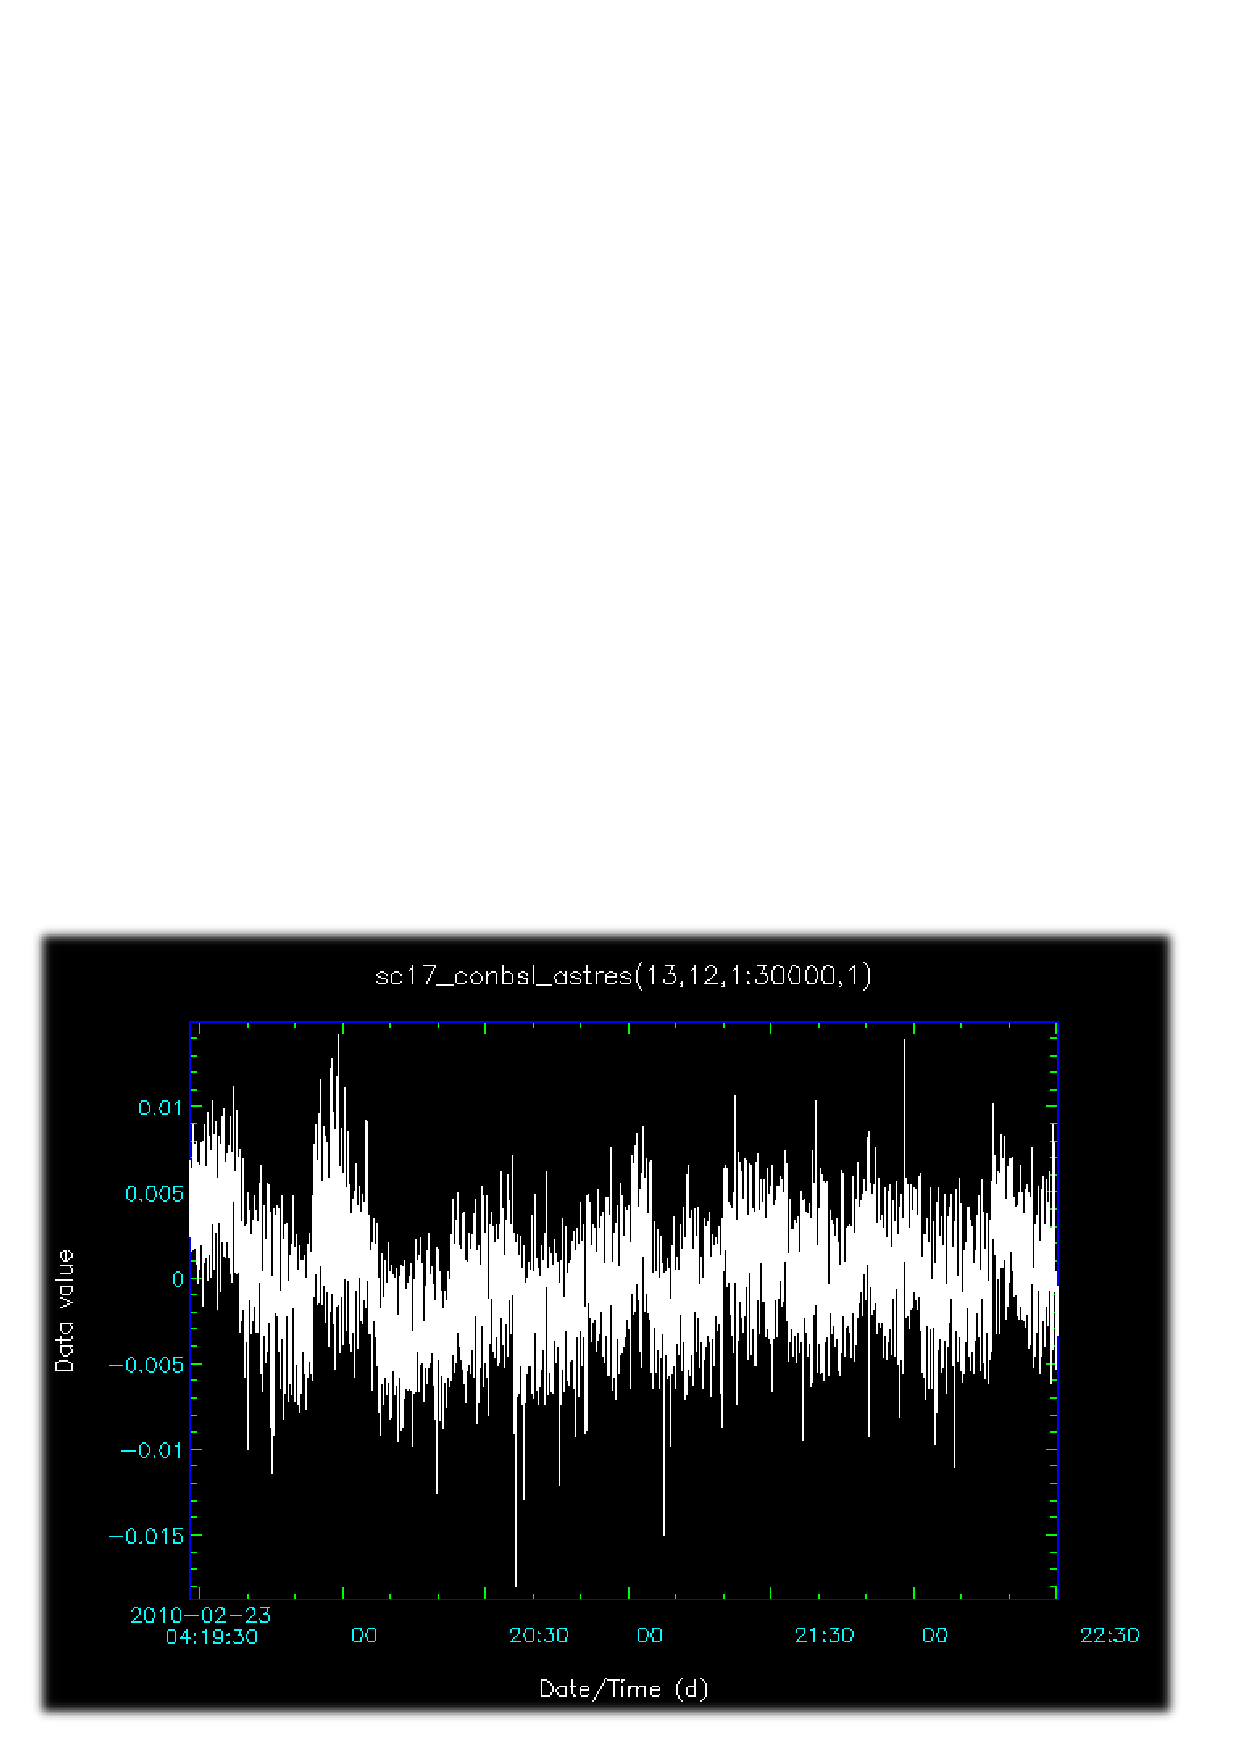
\includegraphics[width=0.30\linewidth]{sc19_conbsl_astres_13_12}
\hspace{0.03\linewidth}
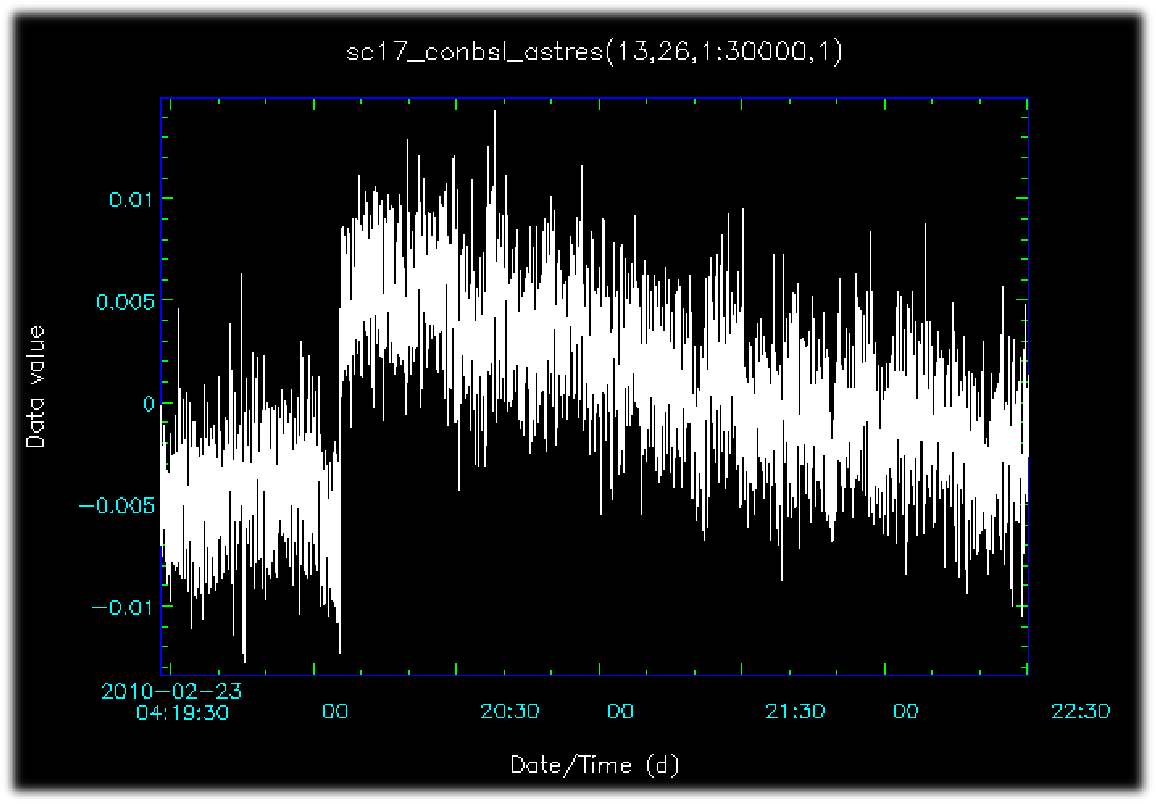
\includegraphics[width=0.30\linewidth]{sc19_conbsl_astres_13_26}
\caption{Sample time-series with a simple common-mode subtracted.}
\label{fig:sampleastres}
\end{center}
\end{figure}
\subsection{\xlabel{samplemaps}Maps}
\label{sec:samplemaps}

Although somewhat outside the scope of this document, after all this
one might wonder what the maps from the various techniques looks like.
Bear in mind that both a manual reduction as well as the mapmaker can
be optimized better than is presented here. Apart from the first map,
all the maps in Fig.\ \ref{fig:samplemaps} are presented with the same
grey-scale stretch and show a 180 $\times$ 180 arcsec region around
CRL\,618.

\begin{figure}[ht]
\begin{center}
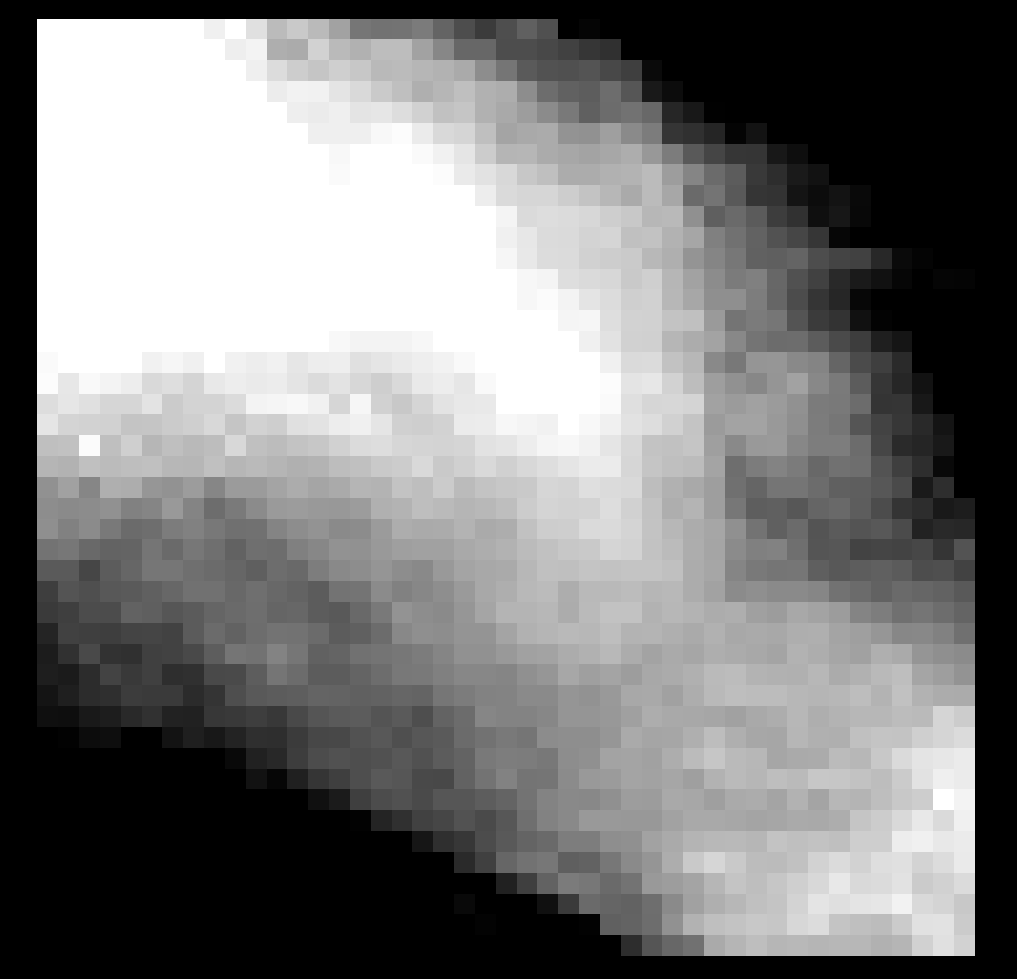
\includegraphics[width=0.45\linewidth]{sc19_con_smallmap}
\hspace{0.03\linewidth}
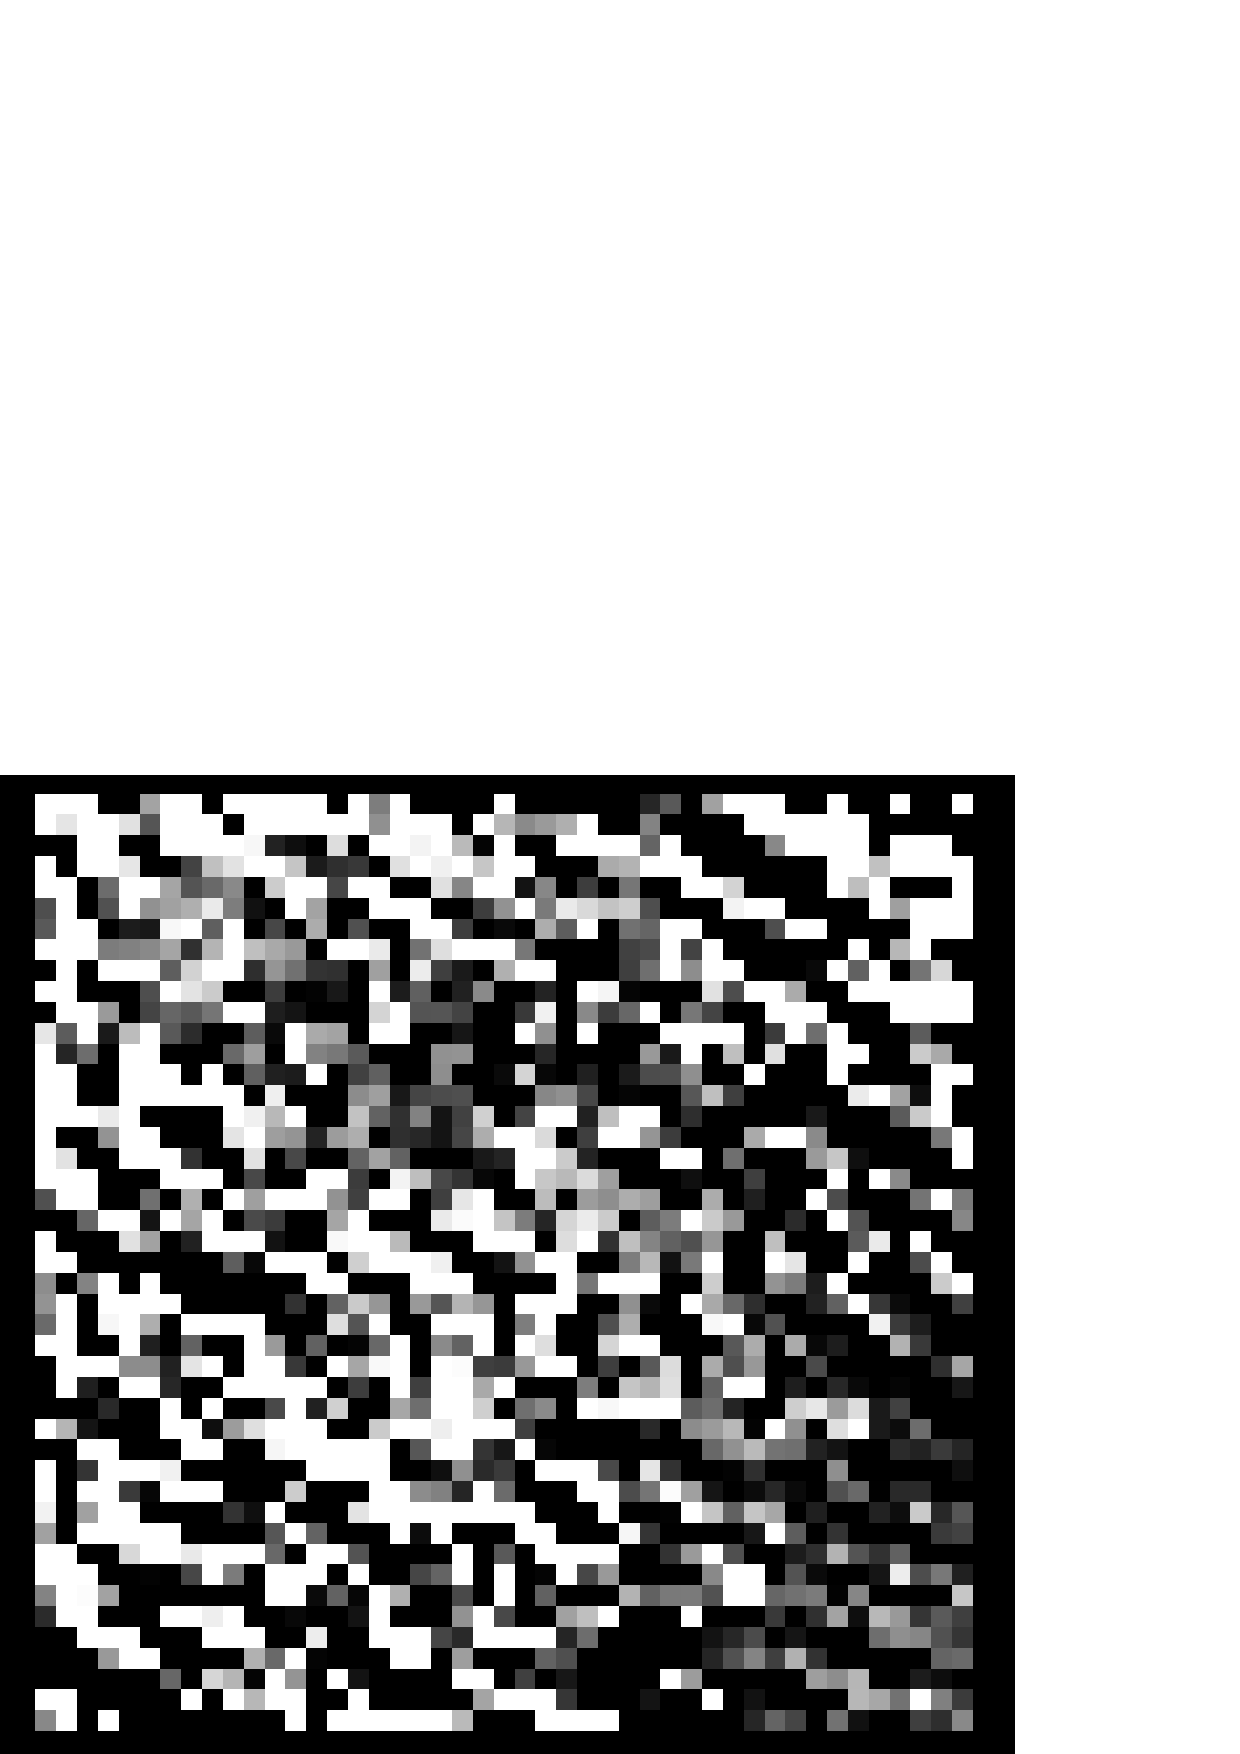
\includegraphics[width=0.45\linewidth]{sc19_conbsl_smallmap}
\includegraphics[width=0.45\linewidth]{sc19_concln_smallmap}
\hspace{0.03\linewidth}
\includegraphics[width=0.45\linewidth]
           {sc19_dimmconfig_bright_compact_smallmap}
\caption{
\textsl{Top left:} Map of the concatenated data;
\textsl{Top right:} After removing a linear baseline from the time series;
\textsl{Bottom left:} After linear baseline, steps, and spike removal;
\textsl{Bottom right:} Iterative map maker with \texttt{dimmconfig\_bright\_compact.lis}
}
\label{fig:samplemaps}
\end{center}
\end{figure}


\newpage
\subsection{\xlabel{script}Sample Common-mode script}
\label{sec:script}

\begin{small}
\begin{terminalv}
(csh)
echo "Remove linear baseline for easy comparison displays"
sc2clean sc17_con sc17_conbsl config=^my_sc2clean_bsl.def

set file = sc17_conbsl

echo "run the DIMM models"
makemap method=iter config=^my_dimmconfig_bright_compact.lis \
        in=${file} out=${file}_map

echo "# Get dimensions"
ndftrace ${file} >& /dev/null
set lbnds = `parget lbound ndftrace | head -1`
set ubnds = `parget ubound ndftrace | head -1`

set xlo =  $lbnds[1]
set xhi =  $ubnds[1]
set ylo =  $lbnds[2]
set yhi =  $ubnds[2]
set zlo =  $lbnds[3]
set zhi =  $ubnds[3]

echo "Find out padding in AST file
ndftrace ${file}_con_ast >& /dev/null
set lbnds = `parget lbound ndftrace | head -1`
set ubnds = `parget ubound ndftrace | head -1`

set zlo2 =  $lbnds[3]
set zhi2 =  $ubnds[3]
set pad = `calc "(${zhi2}-${zhi})/2"`
echo "$pad"
set zlo2 = `calc "${pad}+1"`
set zhi2 = `calc "${zhi}+${pad}"`

echo "Add unpadded part of ast and res model"
add ${file}_con_ast'(,,'${zlo2}':'${zhi2}')' \
    ${file}_con_res'(,,'${zlo2}':'${zhi2}')' ${file}_astres
setorigin ${file}_astres '[0,0,1]'
wcscopy ${file}_astres like=${file} ok=y

echo "Grow the COM back into a cube"
ndfcopy ${file}_con_com'(,,'${zlo2}':'${zhi2}')' \
        temp1 trim
manic  temp1  temp2  axes='[0,1]' \
       lbound=${xlo} ubound=${xhi}
manic temp2 temp_commode axes='[1,0,2]' \
       lbound=${ylo} ubound=${yhi}
setorigin temp_commode  '[0,0,1]'
wcscopy temp_commode like=${file} ok=y

echo "Grow the GAI back into a cube"
manic  ${file}_con_gai'(,,1)'  temp_gain \
       axes='[1,2,0]' lbound=${zlo} ubound=${zhi}
wcscopy temp_gain like=${file} ok=y

echo "Multiply GAI and COM to get the full common-mode cube"
mult temp_gain temp_commode ${file}_commode

echo "Derive 1-centered gain map"
histat ${file}_con_gai'(,,1)'
set median = `parget median histat | head -1`
cdiv  ${file}_con_gai'(,,1)' $median ${file}_gain
\rm temp?.sdf >& /dev/null
\end{terminalv}
\end{small}

\newpage
\section{Notes on Shared Risk Observing}

\subsection{S2SRO FCFs}

Calibration observations were undertaken on a series of secondary
calibrators, which are listed with their SCUBA fluxes in
Table~\ref{tab1}. The data for the FCF calculations were taken between
the 23rd of February and the 14th of March, 2010.

\begin{table}[h]
\caption{Secondary calibrators used for flux calibration of SCUBA-2.
  The flux values are sourced from the references noted in the table. }
\label{tab1}
\begin{center}
\begin{tabular}{|c|c|c|c|c|c|}

\hline
\rule[-1ex]{0pt}{3.5ex} Source & RA(J2000) & DEC(J2000) & 850\micron\
flux / Jy & 450\micron\ flux / Jy & Ref  \\
\hline
\rule[-1ex]{0pt}{3.5ex} HL\,Tau & 04 31 38.4 & +18 13 59.0 & 2.36 $\pm$ 0.24     & 9.9 $\pm$ 2.0 & \cite{flux1}\\
\hline
\rule[-1ex]{0pt}{3.5ex} CRL\,618	& 04 42 53.60 & +36 06 53.7 & 4.7  $\pm$ 0.37   & 12.1 $\pm$ 2.2 & \cite{flux1} \\
\hline
\rule[-1ex]{0pt}{3.5ex} CRL\,2688 & 21 02 18.81 & +36 41 37.7 & 6.39  $\pm$ 0.51  & 30.9 $\pm$ 3.8 & \cite{flux1} \\
\hline
\rule[-1ex]{0pt}{3.5ex} IRC+10216 & 09 47 57.38 & +13 16 43.7 & 8.8  $\pm$ 1.1  & 17.5$\pm$ 4.5 & \cite{flux1} \\
\hline
\rule[-1ex]{0pt}{3.5ex} V883 Ori &  05 38 19  & -07 02 2.0 & 1.34 $\pm$ 0.01     & 7.28 $\pm$ 0.07 & \cite{flux2}   \\
\hline
\rule[-1ex]{0pt}{3.5ex} Alpha Ori & 5 55 10.31 & +07 24 25.4 & 0.628 $\pm$ 0.008  & 1.39 $\pm$ 0.04 & \cite{flux2}  \\
\hline
\rule[-1ex]{0pt}{3.5ex} TW Hydrae & 11 01 51.91 & -34 42 17.0 & 1.37 $\pm$ 0.01 & 3.9 $\pm$ 0.7 & \cite{flux2}  \\
\hline
\rule[-1ex]{0pt}{3.5ex} Arp\,220 & 15 34 57.21 & +23 30 09.5 & 0.668 $\pm$ 0.007  & 2.77 $\pm$ 0.06 & \cite{flux2} \\
\hline

\end{tabular}
\end{center}
\end{table}


The observations were reduced with the mapmaker using the config
dimmconfig\_bright\_compact.lis and post-processed with the \picard\
recipe \drrecipe{SCUBA2\_FCFNEFD}. Figure~\ref{fig:fcfs} shows the 850\micron\ and
450\micron\ \fcfbe\ values for all calibrator observations taken
during the S2SRO period. The resulting mean FCF's in each waveband
are as follows:

\begin{equation}
\mathrm{FCF}_{450} = 400 \pm 90 ~\mathrm{Jy/beam/pW}
\end{equation}
\begin{equation}
\mathrm{FCF}_{850} = 500 \pm 90 ~\mathrm{Jy/beam/pW}
\end{equation}

\begin{figure}
\begin{center}
\includegraphics[width=7cm,angle=90]{sc19_fcf_hist}
\caption{Histograms of the 450\micron\ (left) and 850\micron\ (right)
  \fcfbe\ values calculated for the secondary calibrators observed
  during the S2SRO period.}
\label{fig:fcfs}
\end{center}
\end{figure}

The first note regarding the FCF's produced by the current reduction
is in regard to the picowatt (pW) scale produced by the mapmaker. The
pW scale is dependent on the accuracy of the heater resistance and the
fraction of the heater power which is transferred to the bolometer. At
the time of data release, the effective resistance was not well
described, which induces an uncertainty in the pW scale of the
resultant maps. This resistor value, and therefore the absolute pW
scale, will be determined accurately when the instrument is returned
to operation, and when this is known the new values will be added to
the reduction code. This will affect the pW values of all
observations, and the corresponding FCFs. However, the flux scaling
will be preserved. The FCF values above have been calculated with the
original pW scale.

Secondly, it is obvious that there is a large scatter in the FCFs in
Figure~\ref{fig:fcfs}. It is possible that the variation in the FCFs
is produced by instrument performance changes or inconsistencies in
the way the map-maker reduces the observations. At the time of
release, the source of the scatter was not well understood and
investigation continues. However, it is worth noting that the scatter
between calibrations in an individual night of observations was
sometimes observed to be as high as the scatter over the entire
dataset. No trends were observed as a function of atmospheric
transmission, or time during the night, or over the entire observing
period. It is for this reason that it is advised that the average FCF
values above are used, as opposed to selecting individual calibrations
and using that FCF to calibrate your data.

\subsection{Method for calibrating your data}


It is the recommendation to use the mean \fcfbe\ values
presented in the previous section to calibrate your data. However, if
it is desired to produce an individual FCF from the night of a
particular set of science observations, then the method is described
here.

\begin{enumerate}
\item{Reduce the selected calibration observation using the
\texttt{dimmconfig\_bright\_compact.lis config file}.}
\item{Use \picard's recipe \drrecipe{SCUBA2\_FCFNEFD} on your reduced calibration
    observation. This will produce information to the screen and a
    logfile \texttt{log.fcfnefd} with the FCFs as mentioned above, and an NEFD
    for the observation. \picard\ by default uses fixed FCF's to
    calculate the NEFD. (450\micron: 400 Jy/beam/pW and 850\micron: 500
    Jy/beam/pW). If you wish to get an NEFD using the FCF calculated
    for the individual calibrator you are reducing, add \texttt{USEFCF=1} to
    your parameter file. }
\item{Take your selected FCF and multiply your map by it using \Kappa\
    \cmult.}
\end{enumerate}

\subsection{\xlabel{sroevents}Significant Events}

Part of the risk in S2SRO was that the instrument was being
commissioned in parallel to being used for science
observations. During February and March 2010 a number of events
occurred that will possibly affect the data quality in a good or a bad
way. This section documents these changes to aid in interpreting
unexpected results that may come out of the data reduction process.

\textit{Note:} all dates listed below are UT and are inclusive, and
although setup changes should not affect the calibration they will
affect the number and quality of functioning bolometers.

\subsubsection{Data Files}

Up to 20100219 the first and last file in a scan are dark frames for
science, pointing\footnote{Pointings also have dark frames between
  the data frames in a scan for most of the SRO period.} and focus
observations. From 20100220 to 20100302 the first and last file are
fast flatfield ramps. From 20100303 the first file is a dark frame and
the second and last file are fast ramps. Note noise and discrete flat
fields are different.

\subsubsection{\xlabel{sro_flatfields}Flatfields}
\label{sec:sro:flatfields}

\begin{description}

\item[Beginning of S2SRO -- 20100211] \mbox{}

  Until scan \#17 on 20100211 discrete flatfields were reduced using
  the \param{TABLE} method.

\item[20100211 -- End of S2SRO] \mbox{}

  From scan \#18 on 20100211 discrete flatfields were reduced using
  the \param{POLYNOMIAL} meth. \textit{Note:} the stand alone
  flatfield observations are not used after the fast ramp flatfield
  was implemented 20100223. The fast flatfields are done as part of
  the observations.

\item[20100213 -- 20100215] \mbox{}

  Until scan \#45 the heater step in the discrete flatfield was
  smaller leading to failure of the flatfield on the sky, particular
  at 450. Hence a lot of the flatfields on these dates were in the dark.
  This means less accurate flatfields.

\item[20100220 -- 20100222] \mbox{}

  Fast ramp flatfield used implemented but done in the dark. \smurf\
  uses the discrete flatfields for these dates.

\item[20100223 -- 20100302] \mbox{}

  Fast ramp flatfield on the sky.  \textit{Note:} on 20100223 the data header
  claims the ramp was in the dark but from notes and the heater value
  it was on the sky i.e.\ the dark shutter header was wrong this
  night. \smurf\ knows about this and uses the fast ramp flatfield.

\item[20100303 -- end of S2SRO] \mbox{}

  Fast ramp flatfield used with an initial dark in the
  observations. This dark was used as a sanity check and is not used
  by the map-maker.

\end{description}

Explanatory Notes:

\begin{itemize}
\item Discrete flatfields step through a number of heater values
  rather slowly. The slow speed make the flatfield accuracy and
  quality susceptible to thermal drifts, 1/f noise and weather
  changes. Discrete flatfields were used for flatfielding until
  20100223. Thereafter fast flatfield ramps are done at the start and
  end of every science observation.

\item Fast ramp flatfield uses a fast heater ramp repeated several
  times - this improves the flatfield accuracy and quality.

\item \param{TABLE} and \param{POLYNOMIAL} are two reduction methods
  used for discrete flatfields (fast ramp always uses a polynomial
  method). Due to the lack of dark frame subtraction the \param{TABLE}
  flatfield only used 2 points of the \about10 heater settings in a
  discrete flatfield. Further, the slope from these two points were
  extrapolated far away.  Obviously this affects the flatfield
  accuracy and quality. The flat field calculation should be redone
  using the \param{POLYNOMIAL} method for data taken before
  20100211\footnote{Re-reduce the relevant flatfields using \calcflat\
    and then use \copyflat\ to copy the flatfield into the data files
    before using the map-maker.}.

\end{itemize}

\subsubsection{Setup}

\begin{description}

\item[20100216 -- 20100218] \mbox{}

  s4a detector bias set to 40000 - during the S2SRO the normal s4a value
  was 65000.

\item[20100304 -- end of S2SRO] \mbox{}

  The heater tracking was changed such that the heater is returned to
  the default value each time the shutter was closed. This was done to
  prevents drifts in the heater setting. Such drift affect the
  setup. However, noise observations also reset the heater. Thus the
  heater drift before this adjustment were small and is not believed to
  have affected the data.

\end{description}

\subsubsection{Electronics}

\begin{description}

\item[Beginning of S2SRO -- 20100217] \mbox{}

  A large number of spikes are present in the s4a array data.

\item[20100218 -- end of S2SRO] \mbox{}

  The MCE was changed on the s4a array significantly decreasing the
  number of spikes in the s4a data.

\end{description}

\subsubsection{Weather}

\begin{description}

\item[20100310] \mbox{}

  Very bad seeing: data severely affected

\item[20100311 early evening] \mbox{}
  Bad seeing: data affected

\end{description}

\subsubsection{Telescope}

\begin{description}

\item[early commissioning -- 20091202] \mbox{}

  For early commissioning data it was found that one of the mirrors
  was installed upside down leading to a slightly distorted beam
  shape. This was fixed from 20091203 so care should be taken when
  analysing very early commissioning data found in the archive before
  that date.

\item[Beginning of S2SRO -- 20100225] \mbox{}

  A two component pointing model (utilising only the \texttt{CA} and
  \texttt{IE} terms) was used, leading to large pointing shifts when
  doing large slews. On 20100226 the full eight component model was
  implemented and all-sky pointing improved. This should not affect
  data quality significantly since local pointing would still be
  adequate even with the earlier model.

\end{description}

\section{\xlabel{acronyms}List of acronyms}

\begin{description}

\item[CSO]\quad Caltech Submillimetre Observatory

\item[DIMM]\quad Dynamic Iterative Map-Maker

\item[FCF]\quad Flux Conversion Factor

\item[FWHM]\quad Full-Width at Half-Maximum

\item[GAIA]\quad Graphical Astronomy and Image Analysis Tool

\item[JCMT]\quad James Clerk Maxwell Telescope

\item[NEFD]\quad Noise Equivalent Flux Density

\item[PSF]\quad Point Spread Function

\item[S2SRO]\quad SCUBA-2 Shared Risk Observing which took place in
  February and March 2010.

\item[SCUBA]\quad Submillimetre Common User Bolometer Array

\item[SCUBA-2]\quad Submillimetre Common User Bolometer Array-2

\item[SMURF]\quad Sub-Millimetre User Reduction Facility

\item[S/N]\quad Signal-to-Noise ratio

\item[WVM]\quad Water Vapour radioMeter


\end{description}

\end{document}


